\documentclass[pdflatex,letterpaper,twoside,12pt]{book}

\title             {SKYWARN Systems Reference}
\author            {Maintained by Steve Crow KG4PEQ\\Amateur Radio Coordinator}
\date              {01-Jun-2014}
\newcommand\docver {Version 2014.5}

\usepackage{skywarnbook}
\usepackage{skywarnbook}
\usepackage{minted}
\usemintedstyle{emacs}

\skywarnFormat{printing}
\disableAutoNumbering
\useColorLinks

\hyphenation{SKY-WARN}

\begin{document}
\skywarnTitlePage
\skipToTOC
\skywarnTOC

%%%%%%%%%%%%%%%%%%%%%%%%%%%%%%%%%%%%%%%%%%%%%%%%%%%%%%%%%%%%%%%%%%%%%%%%
%%%%%%%%%%%%%%%%%%%%%%%%%%%%%%%%%%%%%%%%%%%%%%%%%%%%%%%%%%%%%%%%%%%%%%%%
%%%%%%%%%%%%%%%%%%%%%%%%%%%%%%%%%%%%%%%%%%%%%%%%%%%%%%%%%%%%%%%%%%%%%%%%
%%%%%%%%%%%%%%%%%%%%%%%%%%%%%%%%%%%%%%%%%%%%%%%%%%%%%%%%%%%%%%%%%%%%%%%%
%%%%%%%%%%%%%%%%%%%%%%%%%%%%%%%%%%%%%%%%%%%%%%%%%%%%%%%%%%%%%%%%%%%%%%%%
%%%%%%%%%%%%%%%%%%%%%%%%%%%%%%%%%%%%%%%%%%%%%%%%%%%%%%%%%%%%%%%%%%%%%%%%

\chapter{SKYWARN Systems Overview}

%%%%%%%%%%%%%%%%%%%%%%%%%%%%%%%%%%%%%%%%%%%%%%%%%%%%%%%%%%%%%%%%%%%%%%%%

\section{Introduction}

Computers and the Internet play a huge role in the routine operation of the SKYWARN team.  While we exist to provide communications in the event of widespread loss of utilities and other infrastructure, we do capitalize on the use of modern technology in our daily operations.

This manual provides information on the use and maintenance of these systems 
and tools.

%%%%%%%%%%%%%%%%%%%%%%%%%%%%%%%%%%%%%%%%%%%%%%%%%%%%%%%%%%%%%%%%%%%%%%%%

\section{Systems for Net Controllers}\label{nco-systems}

There are five major systems used by SKYWARN Net Control Operators:

\begin{itemize}
\item SKYWARN Operations Portal (``Ops Portal'')
\item SKYWARN Report Management System (RMS)
\item Emergency Managers Weather Information Network (EMWIN)
\item Google Mail
\item Internet Relay Chat (IRC)
\end{itemize}

The first three systems --- Ops Portal, RMS, and EMWIN --- are maintained in-house.  E-mail and chat services are outsourced to third party service providers.

% %%%%%%%%%%%%%%%%%%%%%%%%%%%%%%%%%%%%%%%%%%%%%%%%%%%%%%%%%%%%%%%%%%%%%%%%
% 
% \section{Systems for Responders}\label{responder-systems}
% 
% In addition to the \nameref{nco-systems}, there are additional computing systems and software packages utilized by SKYWARN Responders:
% 
% \begin{itemize}
% \item SKYWARN Responder Desktop
% \item SKYWARN Remote Desktop Environment (RDE)
% \item SKYWARN Responder USB Bundle
% \item SimuAWIPS
% \item Xastir APRS Software
% \end{itemize}
% 
% This documentation will cover the operation of all of these systems.
% 
% %%%%%%%%%%%%%%%%%%%%%%%%%%%%%%%%%%%%%%%%%%%%%%%%%%%%%%%%%%%%%%%%%%%%%%%%
% 
% \section{Systems for Leadership}\label{leadership-systems}
% 
% Leadership team members should be familiar with these systems:
% 
% \begin{itemize}
% \item SDF Public Access Unix System (sdf.org)
% \item Google Admin Console
% \end{itemize}

%%%%%%%%%%%%%%%%%%%%%%%%%%%%%%%%%%%%%%%%%%%%%%%%%%%%%%%%%%%%%%%%%%%%%%%%
%%%%%%%%%%%%%%%%%%%%%%%%%%%%%%%%%%%%%%%%%%%%%%%%%%%%%%%%%%%%%%%%%%%%%%%%
%%%%%%%%%%%%%%%%%%%%%%%%%%%%%%%%%%%%%%%%%%%%%%%%%%%%%%%%%%%%%%%%%%%%%%%%
%%%%%%%%%%%%%%%%%%%%%%%%%%%%%%%%%%%%%%%%%%%%%%%%%%%%%%%%%%%%%%%%%%%%%%%%
%%%%%%%%%%%%%%%%%%%%%%%%%%%%%%%%%%%%%%%%%%%%%%%%%%%%%%%%%%%%%%%%%%%%%%%%
%%%%%%%%%%%%%%%%%%%%%%%%%%%%%%%%%%%%%%%%%%%%%%%%%%%%%%%%%%%%%%%%%%%%%%%%

\chapter{SKYWARN Operations Portal}\label{ops-portal}

%%%%%%%%%%%%%%%%%%%%%%%%%%%%%%%%%%%%%%%%%%%%%%%%%%%%%%%%%%%%%%%%%%%%%%%%

\section{Introduction}

The SKYWARN Ops Portal acts as the main gateway to SKYWARN systems and reference materials for SKYWARN Net Controls, Responders, and Area Managers.  It handles provisioning of user accounts and permissions, provides a roster of team members and functions to maintain that roster, displays activation forecasting information through an interface with our EMWIN system, and serves as an access point for the Net Control Operator Dashboard.

Ops Portal was purpose-built from the ground up to serve the Wakefield SKYWARN amateur radio team.  It is a living system which evolves over time to meet our changing needs.

%%%%%%%%%%%%%%%%%%%%%%%%%%%%%%%%%%%%%%%%%%%%%%%%%%%%%%%%%%%%%%%%%%%%%%%%

\section{Accessing Ops Portal}\label{accessing-ops-portal}

Ops Portal is a web site compatible with most modern web browsers.  The site is designed and tested to operate with the current version of Mozilla Firefox.  Performance and reliability may vary with older versions of Firefox and with any other browser.  The greatest challenges have historically come from users trying to use outdated versions of Microsoft Internet Explorer.  Internet Explorer traditionally does not comply with many web standards, though more recent versions have improved on this.

Before you can access Ops Portal, a user name and password must be issued by a member of the Leadership Team.  This can be accomplished from within Ops Portal, and will be explained later in this documentation.

\begin{figure}[h!]
  \centering
  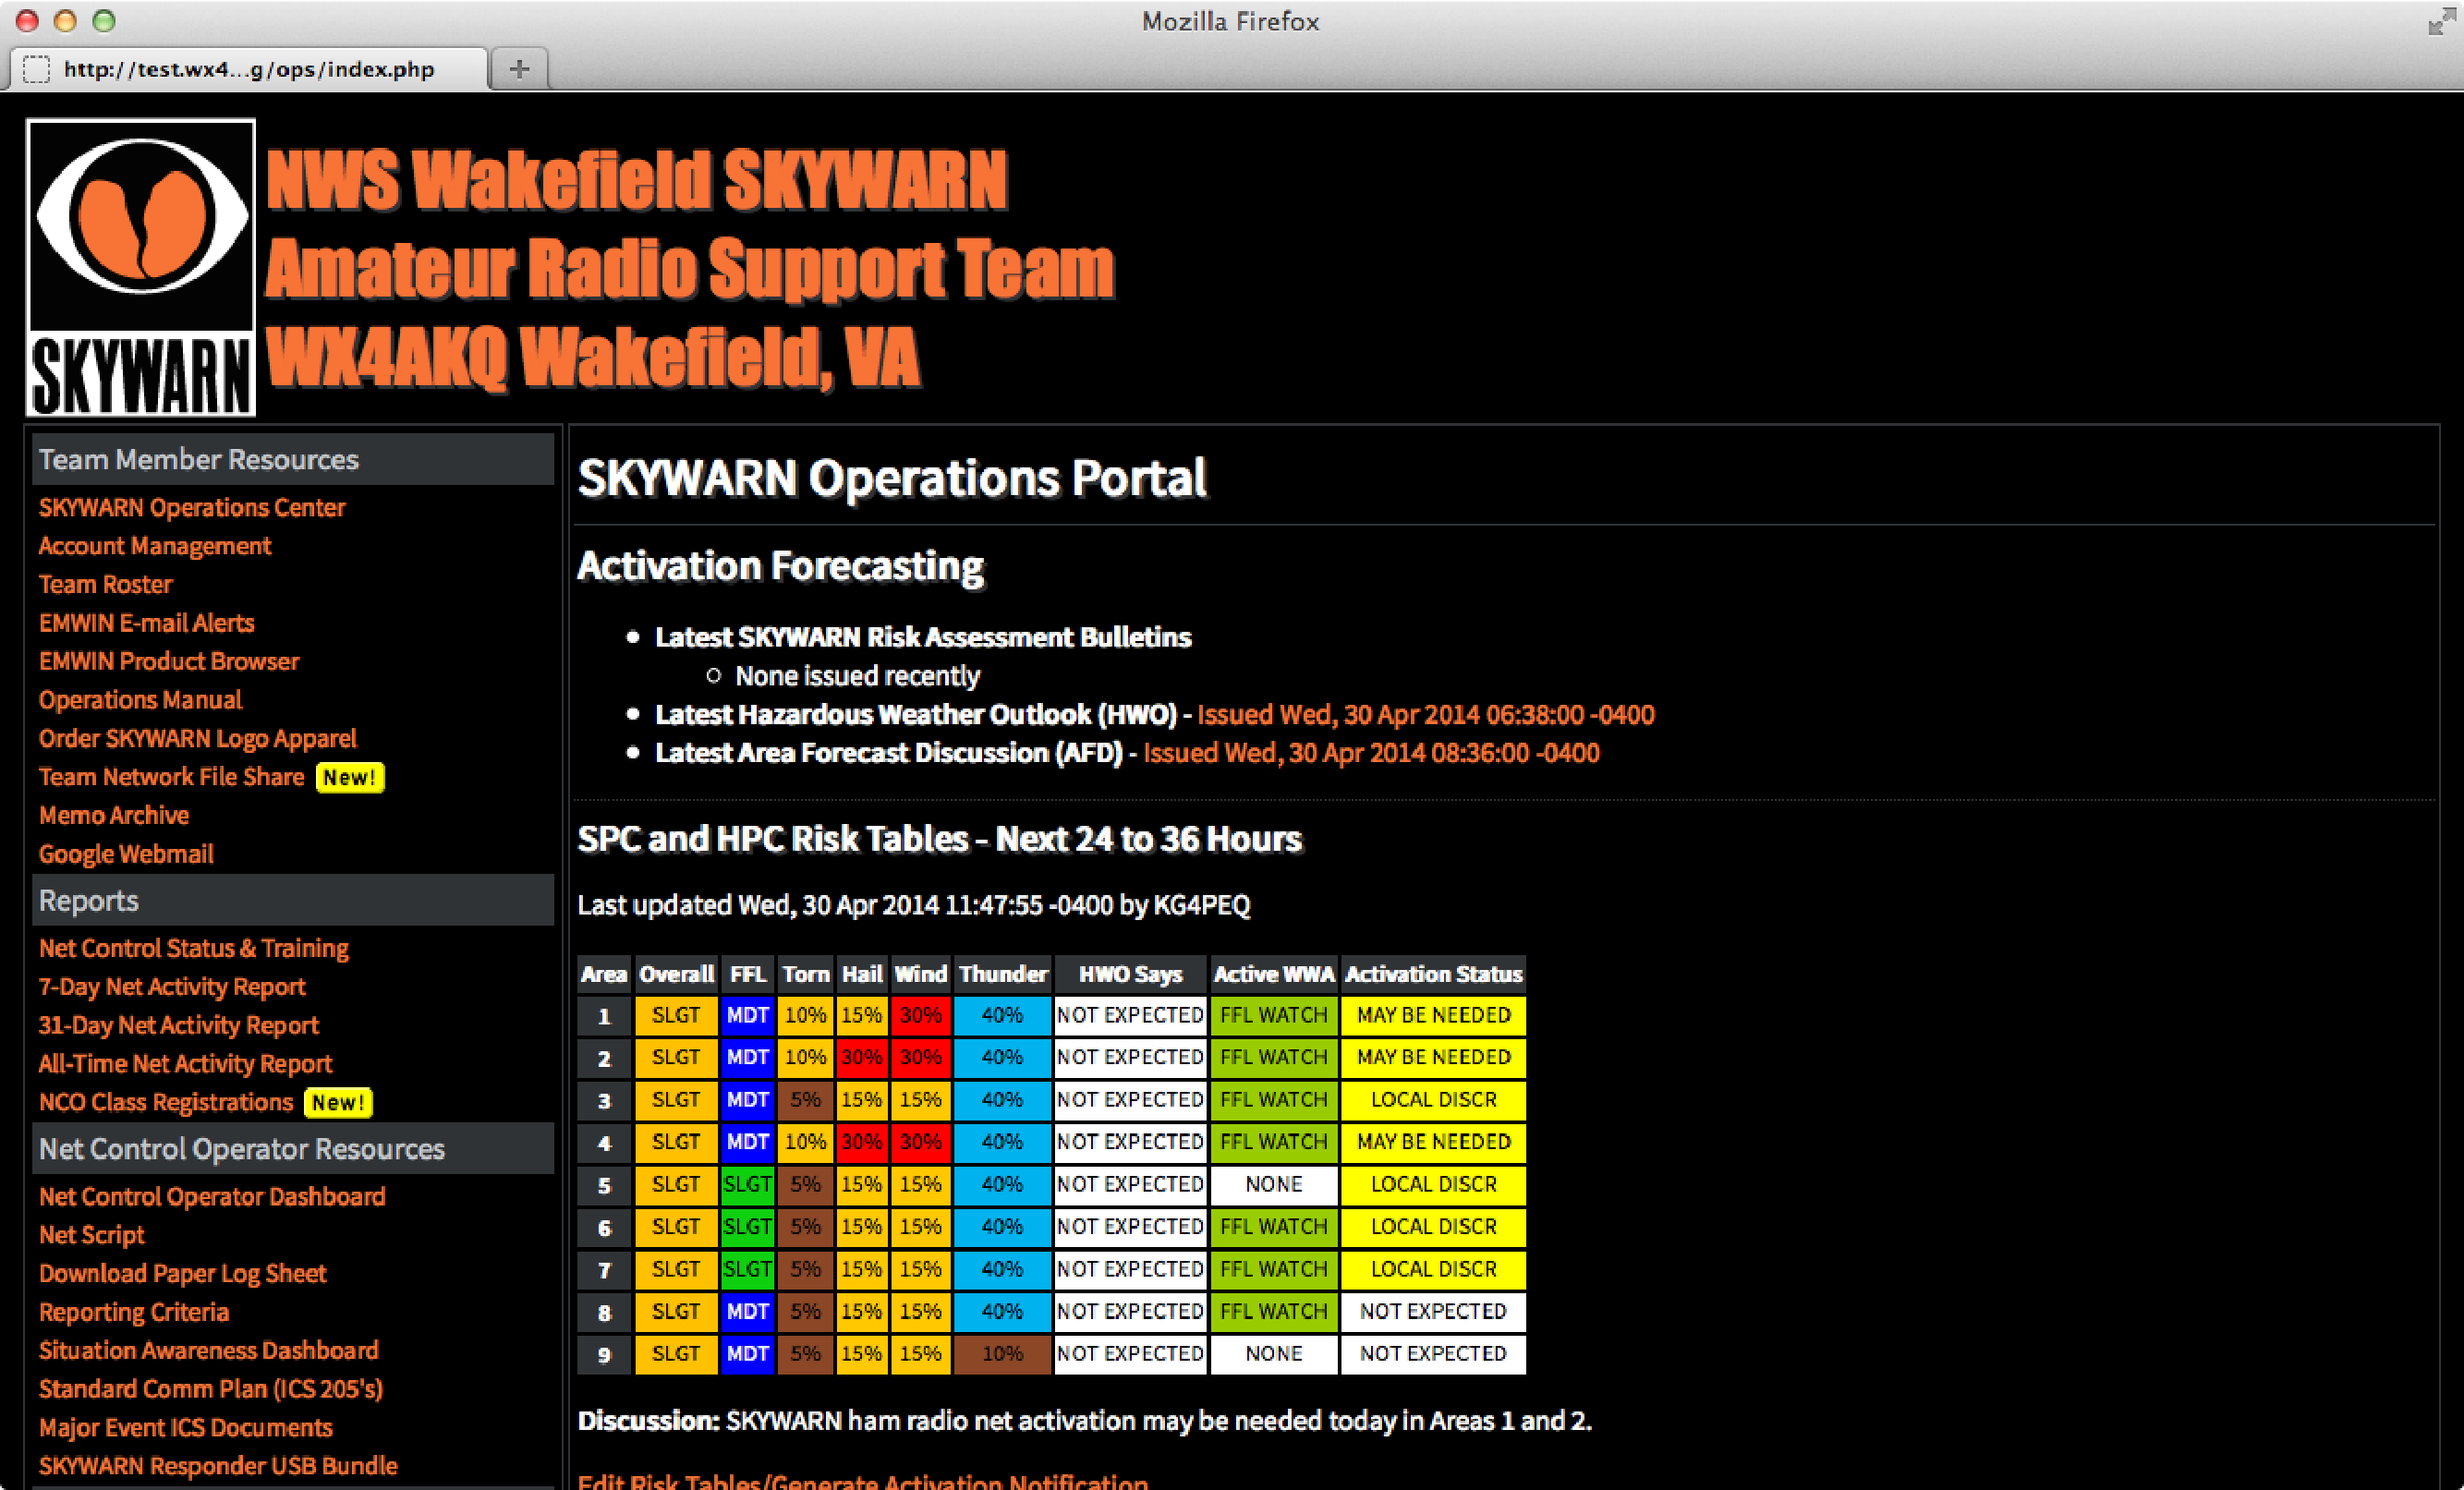
\includegraphics[width=\textwidth,keepaspectratio=true]{img/ops-main-screen}
  \caption{View of the main Ops Portal screen.\label{fig:ops-main-screen}}
\end{figure}

To access Ops Portal, navigate to \href{http://ops.wx4akq.org/}{http://ops.wx4akq.org/}.

The web site will prompt for the user name and password.  Note that both the user name and password are \emph{case sensitive}.  Once valid credentials have been supplied, an Acceptable Use Policy warning screen will appear.  You must agree to the terms and conditions in order to proceed.

\orangebox{Technical Gotcha!}{Cookies must be enabled in order to continue beyond the Acceptable Use Policy screen.  If cookies are not enabled, the user's acceptance of the AUP will not register, and the web site will loop endlessly at the AUP screen.}

The Ops Portal main screen highlights activation forecasting information, including the latest Hazardous Weather Outlook, Area Forecast Discussion, and SKYWARN Risk Tables.  Figure \ref{fig:ops-main-screen} shows the layout of the main screen.  The exact options and information displayed will vary depending on your access privileges.

The navigation bar, along the left side of the screen, contains several categories of links, including general Team Member Links, links of interest to Net Control Operators, Responder Resources, Radar and Model links, Training, Area Manager tools, etc.  Again, the exact categories and links displayed will vary based on your access privileges.

%%%%%%%%%%%%%%%%%%%%%%%%%%%%%%%%%%%%%%%%%%%%%%%%%%%%%%%%%%%%%%%%%%%%%%%%

\section{Updating Personal Information}\label{profile-update}

You are responsible for maintaining your account information within Ops Portal.  The Account Management area provides a password reset utility.

Area Managers also have options to create a new user, change a user's password, manage user permissions, and maintain Situation Awareness Dashboard subscribers.

\orangebox{About Passwords}{Your Ops Portal password provides access specifically to Ops Portal and related services, such as the Situation Awareness Dashboard.  As of May 1, 2014, new team members do not receive Google-hosed SKYWARN e-mail accounts.  Existing team members with these e-mail accounts must contact a member of the Leadership team for password assistance.  These accounts are not managed through Ops Portal or Passport.}

To change your password, click \textbf{Account Management} under \textbf{Team Member Resources} and then select \textbf{Change Password}.

You may also navigate directly to \href{http://ops.wx4akq.org/changepass.php}{http://ops.wx4akq.org/changepass.php}.

Once you submit your new password, you will be immediately prompted to sign back in with your new password.

\orangebox{Good to Know}{Both your user name and password are case-sensitive.  User names should always be entered in all lowercase letters.\\\\If you forget your password, you can reset it with the \href{http://passport.wx4akq.org}{Passport Password Reset Tool}\footnote{http://passport.wx4akq.org/}.  A link to Passport is conveniently located on the public WX4AKQ.org web site, just in case you get locked out.}

Members of the Leadership Team have the ability to reset any user's password without having to go through Passport.  However, team members are strongly encouraged to use Passport for password resets whenever possible, so Leadership resources aren't needlessly tied up with account maintenance tasks.

You are also responsible for keeping your Team Roster information up to date.  There is a section on accessing and using the \nameref{team-roster} on page \pageref{team-roster}, but for now we're specifically interested in how to update your information.

To update, click \textbf{Account Management} under the \textbf{Team Member Resources} category, and then click \textbf{Edit My Roster Entry.}  Fill out all available fields and click \textbf{Update Roster.}  The changes are immediately visible to all team members.  Figure \ref{fig:ops-roster-edit} shows a Team Roster entry being edited.

\begin{figure}[h]
  \centering
  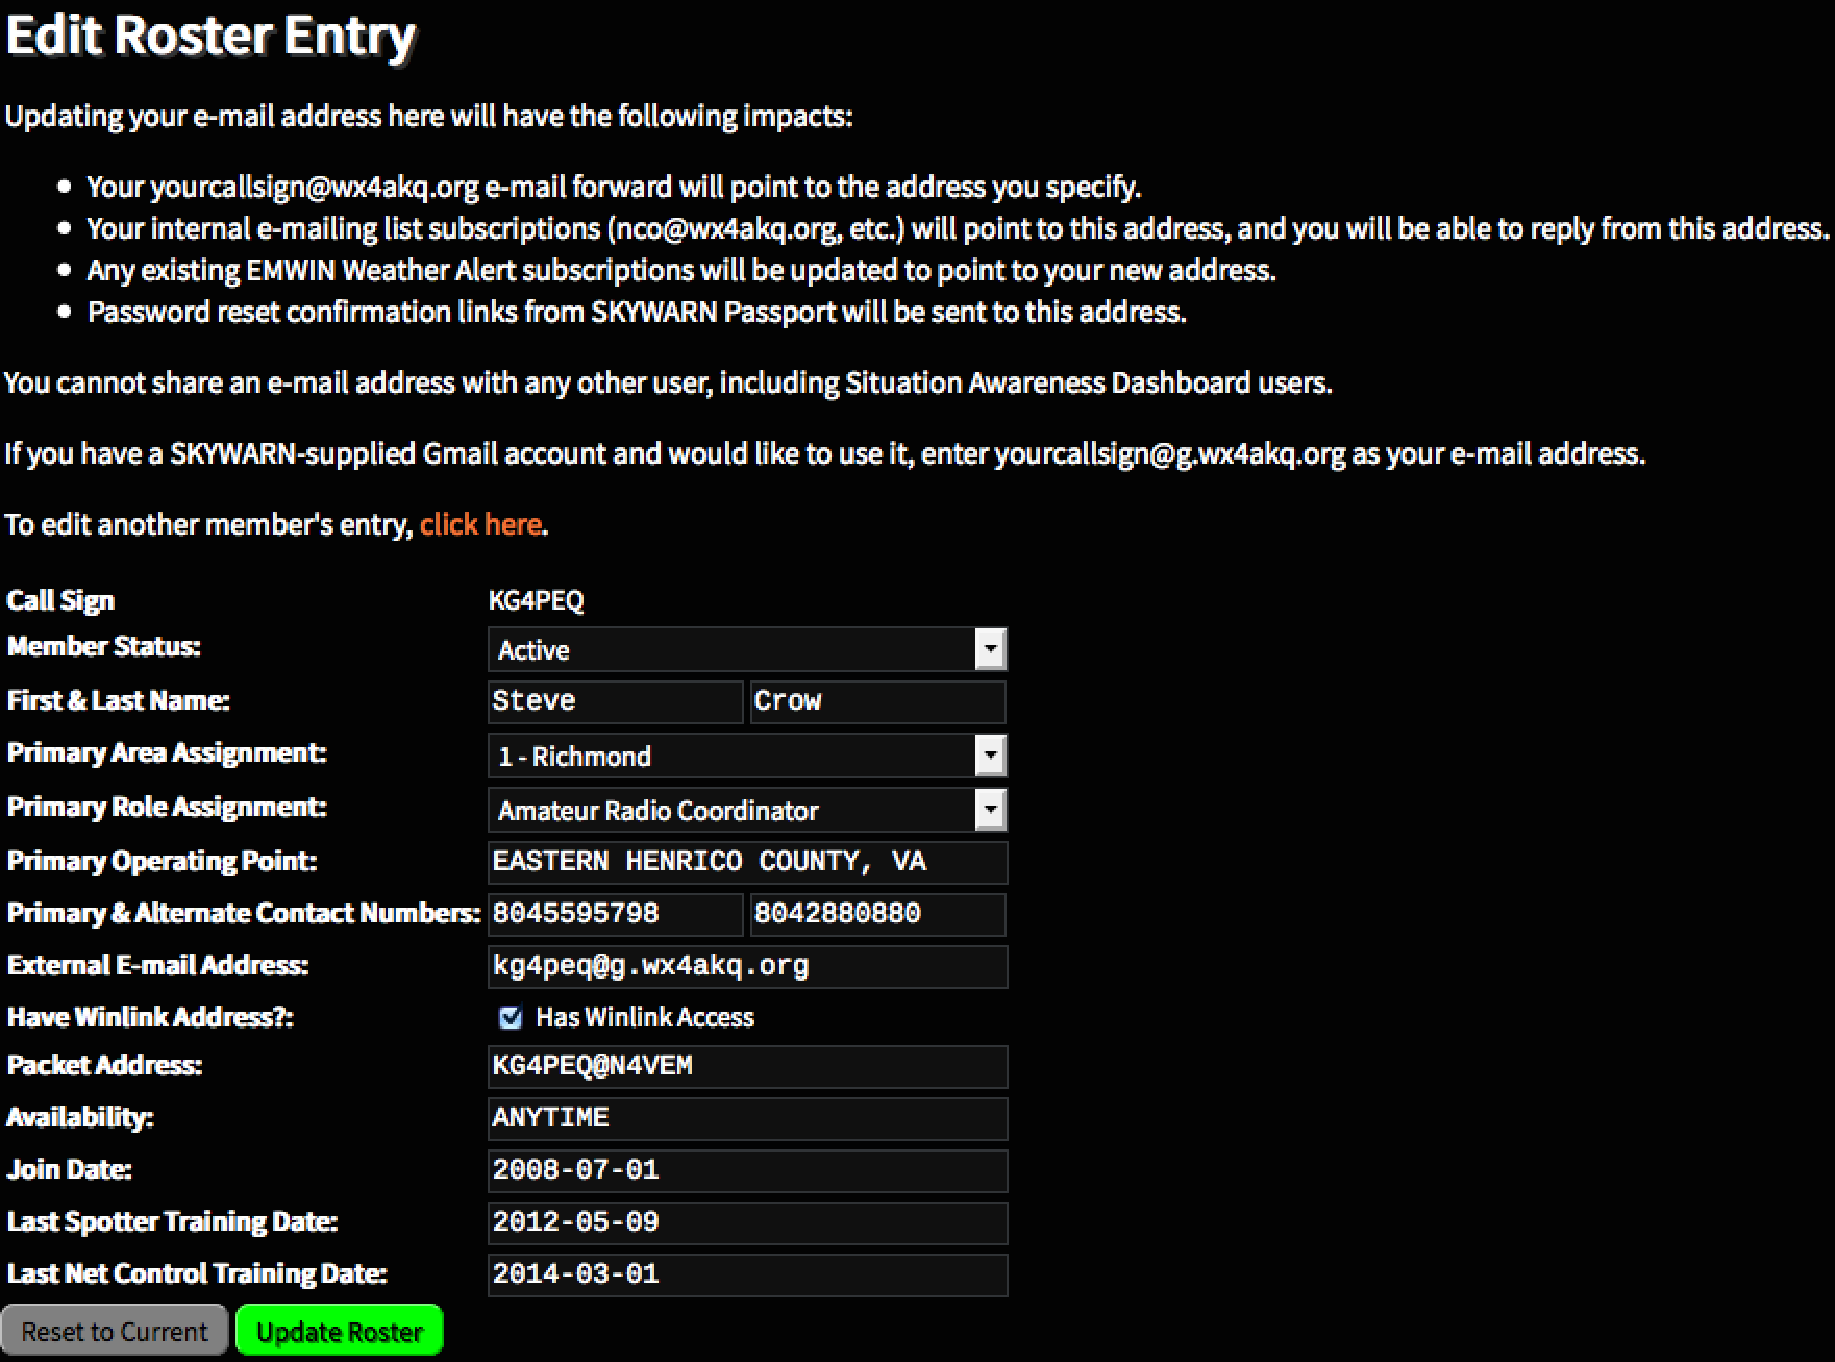
\includegraphics[width=\textwidth,keepaspectratio=true]{img/ops-roster-edit-cropped}
  \caption{Editing a Team Roster entry.\label{fig:ops-roster-edit}}
\end{figure}

The Team Roster should be updated any time your availability, contact information, or other details change.

Leadership Team members have the ability to view and edit any team member's roster information.  Non-Leadership Team members may only edit their own roster entry, but may view anyone's roster information.

%%%%%%%%%%%%%%%%%%%%%%%%%%%%%%%%%%%%%%%%%%%%%%%%%%%%%%%%%%%%%%%%%%%%%%%%

\section{SKYWARN Risk Tables}\label{risk-tables-intro}

The SKYWARN Risk Tables presented on the front page of Ops Portal are an easy-to-use display of generalized information from the Wakefield WFO, Storm Prediction Center (SPC), and NOAA Weather Prediction Center (WPC).  The Risk Tables provide at-a-glance views of the risks of flash flooding, tornadoes, severe hail, severe winds, and more.  Figure \ref{fig:ops-risk-tables-sample} shows a sample Risk Tables product.

The Risk Tables product is \emph{not updated in real-time}.  Area Managers or other members of the Leadership Team must periodically update the information and publish it to the site.  The information in the Risk Tables is considered valid for 18 hours before it is expired, but expired data will continue to display on the site indefinitely.

The Risk Tables are updated through Ops Portal via an \textbf{Edit} link which will appear below the Risk Tables for members of the Leadership Team.  Regular team members, including Net Control Operators, Responders, and most support personnel, cannot edit the Risk Tables.  Figure \ref{fig:ops-risk-tables-editor} shows the Risk Tables Editor.

\orangebox{Shortcut}{\underline{Most} SKYWARN team members will only be concerned with the far right column: \emph{Activation Risk}.  Pay close attention to that column, as it indicates the chances of a SKYWARN activation in each area, as well as the current status of SKYWARN (Activation Requested, Activated, Deactivated).\\\\ The rest of the information in the Risk Tables is targeted at our more ``advanced'' team members.}

\begin{figure}[h]
  \centering
  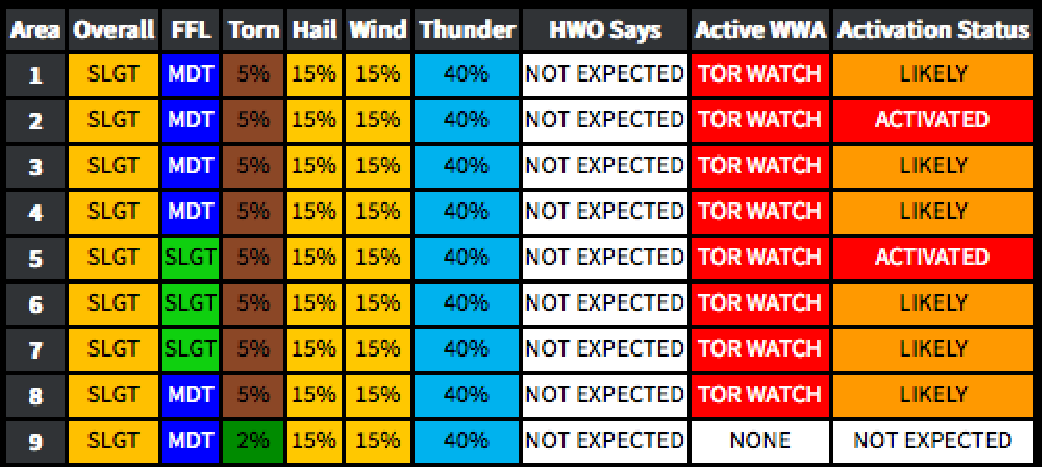
\includegraphics[width=\textwidth,keepaspectratio=true]{img/ops-risk-tables-sample}
  \caption{Sample Risk Tables product.\label{fig:ops-risk-tables-sample}}
\end{figure}

\begin{figure}[h]
  \centering
  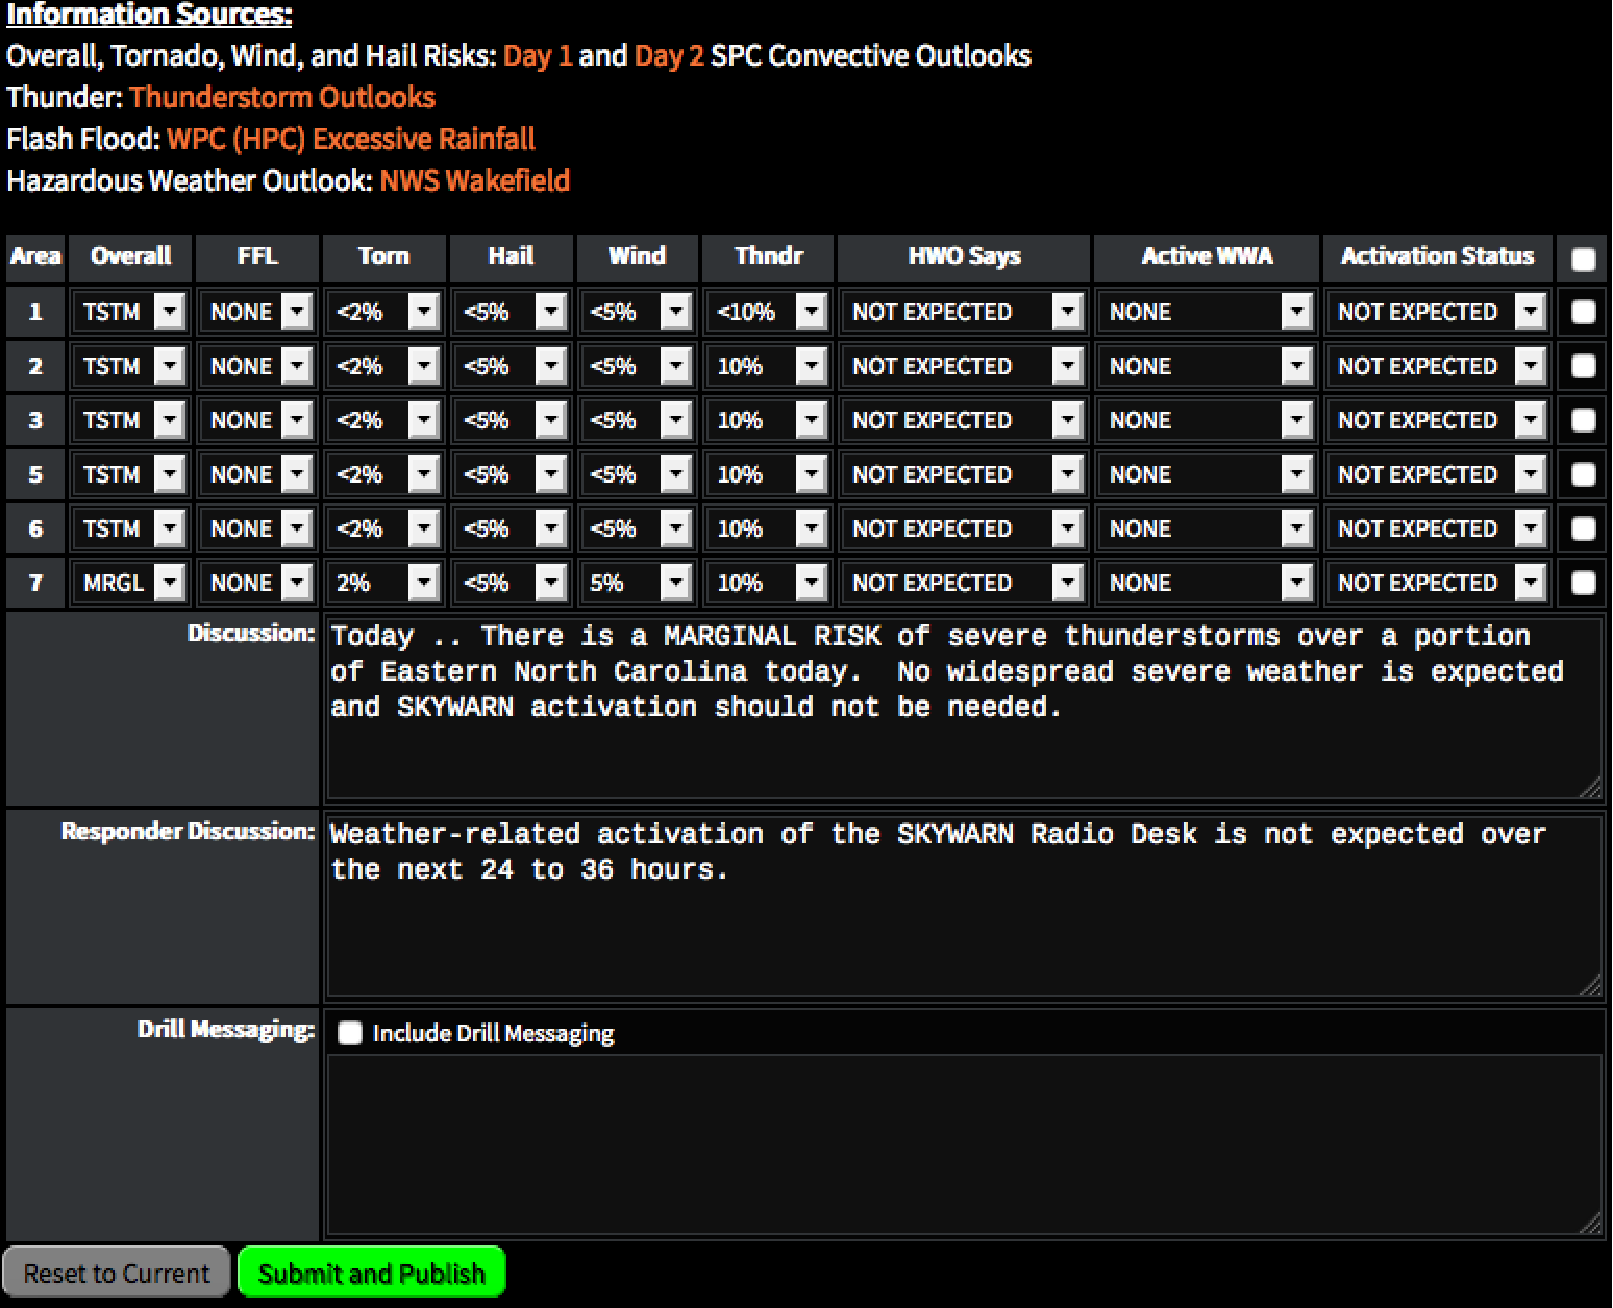
\includegraphics[width=\textwidth,keepaspectratio=true]{img/ops-risk-tables-editor}
  \caption{Leadership Team Risk Tables Editor.\label{fig:ops-risk-tables-editor}}
\end{figure}

Here's a description of each column in the Risk Tables and an explanation of where the information comes from:

\begin{itemize}
\item \textbf{Overall.} This is the overall severe weather risk from the \href{http://www.spc.noaa.gov/products/outlook/day1otlk.html}{SPC Day 1 Convective Outlook}\footnote{http://www.spc.noaa.gov/products/outlook/day1otlk.html}.
\item \textbf{FFL.} This is the flash flood risk from the \href{http://www.hpc.ncep.noaa.gov/qpf/excess_rain.shtml}{WPC Day 1 Excessive Rainfall Discussion}\footnote{http://www.hpc.ncep.noaa.gov/qpf/excess\_rain.shtml}. 
\item \textbf{Torn, Hail, Wind.} These are the categorical risk percentages from the \href{http://www.spc.noaa.gov/products/outlook/day1otlk.html}{SPC Day 1 Convective Outlook}.
\item \textbf{Thndr.} This is the threat percentage from the \href{http://www.spc.noaa.gov/products/exper/enhtstm/}{SPC Enhanced Resolution Thunder Outlook}\footnote{http://www.spc.noaa.gov/products/exper/enhtstm/}.
\item \textbf{HWO Says.}  This is the activation forecast from the ``Spotter Information Statement'' in the latest \href{http://forecast.weather.gov/product.php?site=AKQ&issuedby=AKQ&product=HWO}{Hazardous Weather Outlook}\footnote{http://forecast.weather.gov/product.php?site=AKQ\&issuedby=AKQ\&product=HWO}.
\item \textbf{Active WWA.}  Any active Watch, Warning, or Advisory (WWA) is listed here.  This includes SPC Mesoscale Discussions.
\item \textbf{Activation Risk.}  This is an internally-generated value, based on our assessment of the latest forecast data, weather models, and NWS communication.
\end{itemize}

The Risk Tables also include two free-form \textbf{\emph{Discussion}} fields which can include written communication for Net Control Operators and Responders.  Net Control Operators should read the Discussion text when it is present, as it will contain information on activation timeframes and the specifics of the severe weather threat.

Activation Risk and the Discussion fields are used in the generation of the \emph{SKYWARN Activation Notification} product distributed through our EMWIN notification system.

As of RMS 3.8.3, the far right column of the Risk Tables editor contains a checkbox for each area.  Selecting a checkbox adds EMWIN zone coding to target the selected areas with a notification.  Areas without a check will not be sent a notification when the product is submitted.

%%%%%%%%%%%%%%%%%%%%%%%%%%%%%%%%%%%%%%%%%%%%%%%%%%%%%%%%%%%%%%%%%%%%%%%%

\section{Other Activation Forecast Data in Ops Portal}

The front page of Ops Portal also contains links to the latest Hazardous Weather Outlook, Area Forecast Discussion, and SKYWARN Risk Assessment.

The Hazardous Weather Outlook (HWO) and Area Forecast Discussion (AFD) are published by the National Weather Service Weather Forecast Office (WFO) in Wakefield.  Each product is published several times throughout the day.

The HWO provides a summary of severe weather threats over the next couple of days.  It includes a ``Spotter Information Statement'' which indicates whether Spotter activation is expected over the next four to six hours.

\orangebox{Shortcut}{The Hazardous Weather Outlook provides a summary of severe weather threats over the next couple of days, but the Spotter Information Statement is only valid for the next few hours.  So, an HWO issued in the morning may indicate that Spotter activation is ``not expected'' even though there is a very high threat of severe weather.\\\\Our internal Risk Tables product will help you more easily determine the actual chances of Spotter activation, so you may prefer to use that instead of relying on the HWO.}

The Area Forecast Discussion (AFD) provides a more technical discussion of of the overall weather situation during the next week.  Depending on which NWS forecaster writes the AFD, it may be written in plain English, or it could be full of abbreviations and technical jargon.  Our more advanced team members may find value in the AFD, but the average Net Control probably will not.

Finally, the SKYWARN Risk Assessment Bulletin is an internal product generated by the Leadership Team.  It is a plain-language recap of the severe weather threat, activation timelines, and impact areas in greater detail than the Risk Tables can provide.  The Risk Assessment Bulletin is usually only issued prior to major, widespread, high-impact severe weather events, like winter storms, hurricanes, and significant severe weather outbreaks.

%%%%%%%%%%%%%%%%%%%%%%%%%%%%%%%%%%%%%%%%%%%%%%%%%%%%%%%%%%%%%%%%%%%%%%%%

\section{Memo Archive}

The Memo Archive, shown in Figure \ref{fig:ops-memo-list}, contains an archive of team memos, generally in PDF format.  The memos are named and sorted by date.  Not all memos are preserved here.  These memos are usually limited to policy changes and Leadership Team announcements.  Policy change memos are typically removed once the change has been incorporated into the SKYWARN Operations Manual.

\begin{figure}[h]
  \centering
  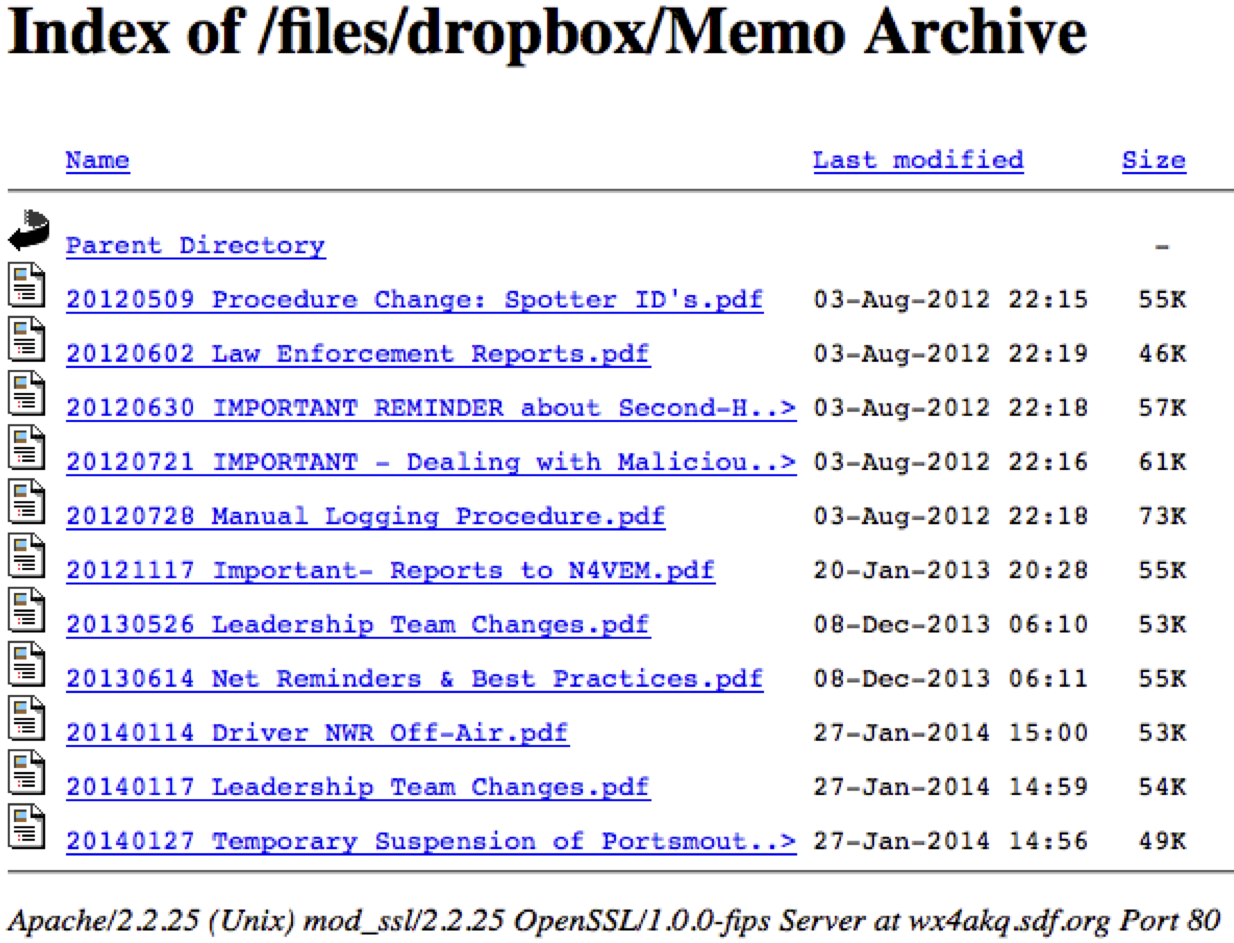
\includegraphics[width=\textwidth,keepaspectratio=true]{img/ops-memo-list-cropped}
  \caption{List of available team memos in the Memo Archive.\label{fig:ops-memo-list}}
\end{figure}

%%%%%%%%%%%%%%%%%%%%%%%%%%%%%%%%%%%%%%%%%%%%%%%%%%%%%%%%%%%%%%%%%%%%%%%%

\section{ICS Documents}

The team's Incident Command System (ICS) documents can be retrieved via Ops Portal.  The most commonly used documents are the ICS-205 Communications Plan and the ICS-205A Communications List.  The team maintains a standard ICS-205 which includes all modes and frequencies designated for team use.  Major, widespread, high-impact events may necessitate the issuance of event-specific ICS documents, which can also be downloaded from Ops Portal as well as our public-facing web site.

ICS documents and their use are well outside the scope of this document.  You can learn more and download form templates at the \href{http://training.fema.gov/EMIWeb/is/ICSResource/}{FEMA ICS Training}\footnote{http://training.fema.gov/EMIWeb/is/ICSResource/} web site.

%%%%%%%%%%%%%%%%%%%%%%%%%%%%%%%%%%%%%%%%%%%%%%%%%%%%%%%%%%%%%%%%%%%%%%%%

\section{Team Roster}\label{team-roster}

The Team Roster is a list of all SKYWARN Amateur Radio team members, including Net Control Operators, Responders, Net Managers, Area Managers, and other support personnel.  It is sorted first by Area Number, and then by last name.

You can update your Team Roster information through the \textbf{Account Management} functions in Ops Portal.  There is more information in the section on \nameref{profile-update} on page \pageref{profile-update}.

The Team Roster contains contact e-mail address, phone numbers, and availability details, along with training details for each team member.  Leadership Team members have access to update training dates and team member roles;  if your training dates or role are incorrect, please contact your Area Manager.

\orangebox{Warning}{The information contained in the Team Roster is \textbf{confidential information} for internal SKYWARN Team use only.  Any distribution or other disclosure of Roster information, in part or in whole, to anyone outside the SKYWARN Amateur Radio team, or use of this information for non-SKYWARN purposes, is not permitted and will lead to disciplinary action up to and including termination of membership.}

%%%%%%%%%%%%%%%%%%%%%%%%%%%%%%%%%%%%%%%%%%%%%%%%%%%%%%%%%%%%%%%%%%%%%%%%

\section{Net Scripts and Log Sheets}

Current Net Scripts and paper Log Sheets are available for download from Ops Portal using the links in the \textbf{Net Control Operator Resources} section.  You should keep several copies of the paper Log Sheets in each location where you may operate a net (home, work, school, in the car, etc).

Information on the use of scripts and log sheets can be found in the \emph{SKYWARN Operations Manual}.

%%%%%%%%%%%%%%%%%%%%%%%%%%%%%%%%%%%%%%%%%%%%%%%%%%%%%%%%%%%%%%%%%%%%%%%%

\section{Leadership Team Functions}

Leadership Team members have access to a few additional functions within Ops Portal:

\begin{itemize}
\item \nameref{ops-create-new-user}
\item \nameref{ops-change-user-password}
\item \nameref{ops-manage-groups}
\item \nameref{ops-delete-user}
\item \nameref{ops-manage-situation}
\end{itemize}

These functions are described in this section.

\subsection{Create a New User}\label{ops-create-new-user}

Creating a new user account is an easy four-step process:

\begin{enumerate}
\item Create the user ID and receive a default password.
\item Assign permission groups.
\item Provide the user ID and default password to the user.
\item Update team member information in the \nameref{team-roster}.
\end{enumerate}

To create a new user, click on \textbf{Account Management} in the \textbf{Team Member Resources} section.  Next to \textbf{Area Manager Tools}, click the \textbf{New User} link and enter the user's amateur call sign and a valid e-mail address.

\orangebox{A note about e-mail}{As of May 1, 2014, new team members do not receive a Google-hosted SKYWARN e-mail address.  Instead, the e-mail address provided during account creation and maintained in the Team Roster will serve as the destination for their \texttt|wx4akq.org| e-mail forward.  For more information, see \nameref{team-email} on page \pageref{team-email}.}

\orangebox{Existing Situation Awareness Dashboard Users}{If the user already has a Situation Awareness Dashboard account under the same e-mail address, a warning will be generated, and you should use the \nameref{sit-account-conversion} to move the existing account to Ops Portal.}

Ops Portal automatically creates a blank Team Roster entry which will need to be filled in later.

Click the \textbf{Add} button to create the account.  The system will generate a default password for the user.  Make a note of this password.

When Ops Portal displays the user's default password, it will provide a link to \textbf{Set group memberships}.  This allows you to set the permissions assigned to the user account and is described in more detail in \nameref{ops-manage-groups} on page \pageref{ops-manage-groups}.

\subsection{Change a User's Password}\label{ops-change-user-password}

Leadership Team Members have the ability to reset a user's password.  Team members requesting a password change should always be directed to use the Passport Password Management Tool whenever possible.

Passport can be accessed at \url{http://passport.wx4akq.org/}.

If it is necessary to manually reset a user's password --- for example, if the user does not have an external e-mail address on file in the \nameref{team-roster} or if they no longer have access to that e-mail address --- then the \textbf{Reset a User's Password} function in \textbf{Account Management} may be used.

\orangebox{Password Resets for Situation Awareness Dashboard Users}{Situation Awareness Dashboard users \emph{must} use Passport to reset their passwords.  The \textbf{Reset a User's Password} function in Ops Portal will only work for Ops Portal logins.}

\subsection{View and Manage Permission Groups}\label{ops-manage-groups}

Permission groups can be managed by clicking on the \textbf{Manage Groups} link in the \textbf{Account Management} area.

Ops Portal currently supports seven permission groups:

\begin{itemize}
\item \verb|admin| - Administrative users.  Currently, this permission group is not used;  all administrative functions are available to \verb|leadership| group members.
\item \verb|leadership| - Leadership Team.  Includes Area Managers, Assistant Area Managers, and Net Managers.  Setting this permission group unlocks the ability to update the \nameref{risk-tables-intro}, enables access to account provisioning and maintenance tools, and unlocks the ability to \nameref{dash-rms-settings}.
\item \verb|responders| - Anyone who may operate the SKYWARN Radio Desk should be assigned to this permission group.
\item \verb|nco| - Net Control Operators.  Anyone who needs access to the NCO Dashboard must be assigned to this permission group.
\item \verb|tech| - Tech Team.  Not currently used.
\item \verb|testserver| - Provides access to the test web server.
\item \verb|ve| - VE Team.  Not currently used.
\end{itemize}

There are also individual permission groups for each SKYWARN Operating Area, primarily used for mailing list subscriptions.

\orangebox{Tech Talk: How Permissions Work}{Permission assignments are stored two places --- in a MySQL database, and in the \texttt{/auth/.htgroups} file on the web server.\\
\\When authoring web pages for Ops Portal and/or the NCO Dashboard, the \texttt{requireGroups()} function\footnote{Provided by \texttt{resources/includes.php}} can be used to restrict access to a specific group.  This function accepts an array of access classes, for example:\\
\\\texttt{requireGroups(array(`responders`,`tech`));}\\\\An Apache \texttt{.htaccess} file can also be used to restrict access to a folder or file, which is the method used for the online File Library:\\\\\texttt{<files *.pdf>\\require group responders\\</files>} }

Changes to group subscriptions here will automatically update the corresponding mailing list subscriptions, using the external e-mail address provided in the \nameref{team-roster}.  That is, if adding user AB1CDE to the ``area1'' permission group, AB1CDE's e-mail address will be automatically subscribed to the ``area1'' mailing list.  For more information, see \nameref{mailing-lists} on page \pageref{mailing-lists}.

\subsection{Delete a User}\label{ops-delete-user}

Deleting a user immediately removes their access to Ops Portal, deletes their EMWIN E-mail Weather Alert subscriptions, and purges their \nameref{team-roster} entry.  This data cannot be recovered.

If the outgoing team member would like to retain their EMWIN E-mail Weather Alert subscriptions and convert to a \nameref{sit-dashboard} account, see the instructions in \nameref{sit-account-conversion} on page \pageref{sit-account-conversion}.  This conversion must be completed \emph{before} deleting the Ops Portal login.

\subsection{Manage Situation Awareness Dashboard Users}\label{ops-manage-situation}

The \textbf{Account Management} area of Ops Portal includes functions for managing subscriptions to the \nameref{sit-dashboard}.  These functions and other related tasks are described in great detail in the Situation Awareness Dashboard \nameref{sit-leadership-functions} section starting on page \pageref{sit-leadership-functions}.

%%%%%%%%%%%%%%%%%%%%%%%%%%%%%%%%%%%%%%%%%%%%%%%%%%%%%%%%%%%%%%%%%%%%%%%%
%%%%%%%%%%%%%%%%%%%%%%%%%%%%%%%%%%%%%%%%%%%%%%%%%%%%%%%%%%%%%%%%%%%%%%%%
%%%%%%%%%%%%%%%%%%%%%%%%%%%%%%%%%%%%%%%%%%%%%%%%%%%%%%%%%%%%%%%%%%%%%%%%
%%%%%%%%%%%%%%%%%%%%%%%%%%%%%%%%%%%%%%%%%%%%%%%%%%%%%%%%%%%%%%%%%%%%%%%%
%%%%%%%%%%%%%%%%%%%%%%%%%%%%%%%%%%%%%%%%%%%%%%%%%%%%%%%%%%%%%%%%%%%%%%%%
%%%%%%%%%%%%%%%%%%%%%%%%%%%%%%%%%%%%%%%%%%%%%%%%%%%%%%%%%%%%%%%%%%%%%%%%

\chapter{SKYWARN RMS}\label{rms}

%%%%%%%%%%%%%%%%%%%%%%%%%%%%%%%%%%%%%%%%%%%%%%%%%%%%%%%%%%%%%%%%%%%%%%%%

\section{Introduction}

The SKYWARN Report Management System, or RMS, is the underlying mechanism by which net reports are collected, logged, relayed, and archived.

The user interface to RMS consists of two main systems:

\begin{itemize}
\item \nameref{nco-dashboard}
\item \nameref{sit-dashboard}
\end{itemize}

All Net Control Operators, Responders, and Leadership Team members have access to the NCO Dashboard, which includes access to the net log archive with minimal restrictions.  The Situation Awareness Dashboard provides certain external users view-only access to the net logs.

%%%%%%%%%%%%%%%%%%%%%%%%%%%%%%%%%%%%%%%%%%%%%%%%%%%%%%%%%%%%%%%%%%%%%%%%

\section{RMS Report Workflow}

The general flow of reports through RMS is as follows:

\begin{enumerate}
\item Reports are collected from Spotters via SKYWARN nets.
\item A report is created in the NCO Dashboard.
  \begin{itemize}
  \item Reports include time stamps for the event and report.
  \item The Spotter call sign and Spotter training status are captured.
  \item Location and report details are captured in free-form text format.
  \item Routing information is specified in the report, including destination office and relay mechanism (phone, e-mail, packet, or automatic release).
  \end{itemize}
\item Report is queued for release for a period of several minutes to allow adequate time for editing.
\item Report is systematically ``released'' from the queue.
  \begin{itemize}
  \item Reports which meet established reporting criteria are automatically routed to the specified office via e-mail.
  \item NWS personnel can respond to reports with acknowledgements or requests for more information by replying to the report.  The report will be routed to the Net Control who took the report.
  \item Reports which do not meet established reporting criteria are not routed to NWS.
  \end{itemize}
\item Reports are permanently archived in a server-side database.
\end{enumerate}

%%%%%%%%%%%%%%%%%%%%%%%%%%%%%%%%%%%%%%%%%%%%%%%%%%%%%%%%%%%%%%%%%%%%%%%%

\section{Interacting with RMS}

RMS records are not usually manipulated directly, though anyone with the proper access to the database server can execute the appropriate MySQL commands to manipulate the database.

Rather than trying to gain direct access, users should take advantage of the various reporting tools which exist within Ops Portal, the NCO Dashboard, and the Situation Awareness Dashboard.

%%%%%%%%%%%%%%%%%%%%%%%%%%%%%%%%%%%%%%%%%%%%%%%%%%%%%%%%%%%%%%%%%%%%%%%%

\section{Supported Offices}\label{rms-offices}

RMS is capable of electronically transmitting reports to our WFO and all WFO's which share a boundary with the Wakefield CWA.  The list of supported offices is:

\begin{itemize}
\item AKQ - Wakefield, VA
\item LWX - Sterling, VA
\item MHX - Newport/Morehead City, NC
\item PHI - Mt. Holly, NJ
\item RAH - Raleigh, NC
\item RNK - Blacksburg, VA
\end{itemize}

For routine reports, there is usually no need to manually relay reports to these WFO's.  If a WFO experiences a communications outage, another relay mechanism must be used.

%%%%%%%%%%%%%%%%%%%%%%%%%%%%%%%%%%%%%%%%%%%%%%%%%%%%%%%%%%%%%%%%%%%%%%%%

\section{Batch Mode}\label{rms-batch-mode}

RMS normally releases reports individually as the Release Delay expires.  For most severe weather events, this is the desired behavior.

Some weather events, specifically winter storms, generate a high volume of reports which are not necessarily time-sensitive.  To minimize the number of individual e-mails that go to the National Weather Service, RMS has a Batch Mode option.

In Batch Mode, reports are ``scooped up'' into one digest-style report once every 30 minutes.  Each NWS office gets its own digest.  Reports shown in the NCO Dashboard \nameref{dash-log-viewer} will still count down from the specified Release Delay, but will not be released from the system until the next batch process runs, \emph{after} the countdown timer reaches zero.

If necessary, it is possible to \nameref{manual-release} before the batch process runs.

Batch Mode can be turned on via the \nameref{dash-rms-settings} option in the NCO Dashboard.

%%%%%%%%%%%%%%%%%%%%%%%%%%%%%%%%%%%%%%%%%%%%%%%%%%%%%%%%%%%%%%%%%%%%%%%%

\section{NWS Replies to RMS Reports}\label{nws-replies}

NWS employees may reply to reports submitted through RMS.  These replies will be routed to the Net Control Operator's \texttt{callsign@wx4akq.org} e-mail address, which will ultimately be forwarded to the e-mail address specified in the Team Roster.  NCO's should closely monitor their e-mail for the duration of their service as a Net Control Operator, and for a period of a few hours thereafter, to handle any requests from NWS employees.

For more information, see \nameref{team-roster} on page \pageref{team-roster}, and \nameref{team-email} on page \pageref{team-email}.

%%%%%%%%%%%%%%%%%%%%%%%%%%%%%%%%%%%%%%%%%%%%%%%%%%%%%%%%%%%%%%%%%%%%%%%%
%%%%%%%%%%%%%%%%%%%%%%%%%%%%%%%%%%%%%%%%%%%%%%%%%%%%%%%%%%%%%%%%%%%%%%%%
%%%%%%%%%%%%%%%%%%%%%%%%%%%%%%%%%%%%%%%%%%%%%%%%%%%%%%%%%%%%%%%%%%%%%%%%
%%%%%%%%%%%%%%%%%%%%%%%%%%%%%%%%%%%%%%%%%%%%%%%%%%%%%%%%%%%%%%%%%%%%%%%%
%%%%%%%%%%%%%%%%%%%%%%%%%%%%%%%%%%%%%%%%%%%%%%%%%%%%%%%%%%%%%%%%%%%%%%%%
%%%%%%%%%%%%%%%%%%%%%%%%%%%%%%%%%%%%%%%%%%%%%%%%%%%%%%%%%%%%%%%%%%%%%%%%

\chapter{Team Member E-mail Services}\label{team-email}

\section{Team Members Provisioned before May 1, 2014}

Team members provisioned prior to May 1, 2014 were given Google-hosted SKYWARN e-mail accounts.  These accounts are part of a free 500-license \href{http://www.google.com/a}{Google Apps} account.  Team members may keep these accounts.  Passwords are managed through the Google Appls control panel at \href{http://www.google.com/a/wx4akq.org}{http://www.google.com/a/wx4akq.org}.

Team members will need to list their \texttt{@wx4akq.org} e-mail address in the \nameref{team-roster} in order to receive e-mail at these Google accounts.

\section{Team Members Provisioned on and after May 1, 2014}

Team members provisioned on and after May 1, 2014 will not receive a Google-hosted SKYWARN e-mail account.  Their \texttt{@wx4akq.org} e-mail address will be a virtual forward to the external e-mail address provided in the \nameref{team-roster}.

Changing the e-mail address in the \nameref{team-roster} will automatically update the virtual e-mail forward.

\section{Named E-mail Accounts}\label{named-email}

Members of the Leadership Team, determined by a membership in the ``leadership'' permission group in Ops Portal, will receive a named e-mail address in the form of \texttt{FirstName.LastName@wx4akq.org} in addition to their \texttt{callsign@wx4akq.org} e-mail address.  The name used to create the named account will be determined by their first and last name listed in the Team Roster.

For more information, see \nameref{ops-manage-groups} on page \pageref{ops-manage-groups}, and \nameref{team-roster} on page \pageref{team-roster}.

\section{Permanent Forwards}\label{perm-forwards}

Permanent forwards, such as \texttt{info@wx4akq.org} can be specified in the e-mail server's virtual user table file, \verb|/etc/postfix/virtual|.  Permanent forwards should be listed \emph{below} the \verb|### Ops_Aliases_End| delimiter, otherwise they may be lost the next time the virtual user table is refreshed.

Running the \verb|postmap /etc/postfix/virtual| command is required after directly editing the virtual user table.

\section{Team Mailing Lists}\label{mailing-lists}

Mailing lists are maintained with the \href{http://www.list.org/}{GNU Mailman} mailing list software.  Custom scripts tie mailing list subscriptions directly to the permission group selections made in Ops Portal and the e-mail address listed for each team member in the \nameref{team-roster}.

Messages from non-subscribed e-mail addresses will go into moderation and must be approved.  This and other list management functions can be accomplished through the Mailman web interface at \href{http://www.wx4akq.org/mailman/admin}{http://www.wx4akq.org/mailman/admin}.

\orangebox{Messages from Non-Subscribed E-mail Addresses}{If someone sends a message to a private team mailing list, such as the \texttt{nco@wx4akq.org} list, or one of the individual Area mailing lists, the message may be approved but the user should \emph{never} be added to the mailing list, and great care should be exercised in adding the user to the auto-accept list.}

%%%%%%%%%%%%%%%%%%%%%%%%%%%%%%%%%%%%%%%%%%%%%%%%%%%%%%%%%%%%%%%%%%%%%%%%
%%%%%%%%%%%%%%%%%%%%%%%%%%%%%%%%%%%%%%%%%%%%%%%%%%%%%%%%%%%%%%%%%%%%%%%%
%%%%%%%%%%%%%%%%%%%%%%%%%%%%%%%%%%%%%%%%%%%%%%%%%%%%%%%%%%%%%%%%%%%%%%%%
%%%%%%%%%%%%%%%%%%%%%%%%%%%%%%%%%%%%%%%%%%%%%%%%%%%%%%%%%%%%%%%%%%%%%%%%
%%%%%%%%%%%%%%%%%%%%%%%%%%%%%%%%%%%%%%%%%%%%%%%%%%%%%%%%%%%%%%%%%%%%%%%%
%%%%%%%%%%%%%%%%%%%%%%%%%%%%%%%%%%%%%%%%%%%%%%%%%%%%%%%%%%%%%%%%%%%%%%%%

\chapter{NCO Dashboard}\label{nco-dashboard}

\section{Introduction}

The Net Control Operator Dashboard is the primary means of interacting with \nameref{rms}.  The NCO Dashboard provides a mechanism for logging reports from Spotters and filing follow-ups to previous reports.  Behind the scenes, RMS handles the automatic release and electronic relay of reports to the National Weather Service.

In the course of routine SKYWARN operations, Net Control Operators usually do not need to be concerned with using the telephone, e-mail, e-Spotter, or other reporting methods to send reports to the National Weather Service.  RMS takes care of it all!

\orangebox{Reminder}{While a majority of Spotter reports only need to be logged and electronically relayed by RMS, remember that urgent reports --- such as tornadoes, funnel clouds, rotating wall clouds, injuries, or fatalities --- must still be relayed directly to NWS personnel by telephone, \emph{in addition to} the electronic logging provided by the NCO Dashboard and RMS.}

The NCO Dashboard is designed to put the most important information in one place, right at the fingertips of NCO's and Responders.  In addition to entering and viewing Spotter reports, the NCO Dashboard also provides quick access to local Team Roster information, local SKYWARN frequencies and repeater commands, a list of current Watches, Warnings, and Advisories (WWA), and an e-mail tool for sending quick messages directly to NWS offices.

%%%%%%%%%%%%%%%%%%%%%%%%%%%%%%%%%%%%%%%%%%%%%%%%%%%%%%%%%%%%%%%%%%%%%%%%

\section{Accessing NCO Dashboard}

The NCO Dashboard is a part of \nameref{ops-portal}.  To access the NCO Dashboard, first log in to Ops Portal, then click the \textbf{NCO Dashboard} link in the \textbf{Net Control Operator Resources} section.

For more information on logging in to Ops Portal, see \nameref{accessing-ops-portal} on page \pageref{accessing-ops-portal}.

The default view of the NCO Dashboard is in Figure \ref{fig:dash-main-screen} on page \pageref{fig:dash-main-screen}.

\begin{figure}[h]
  \centering
  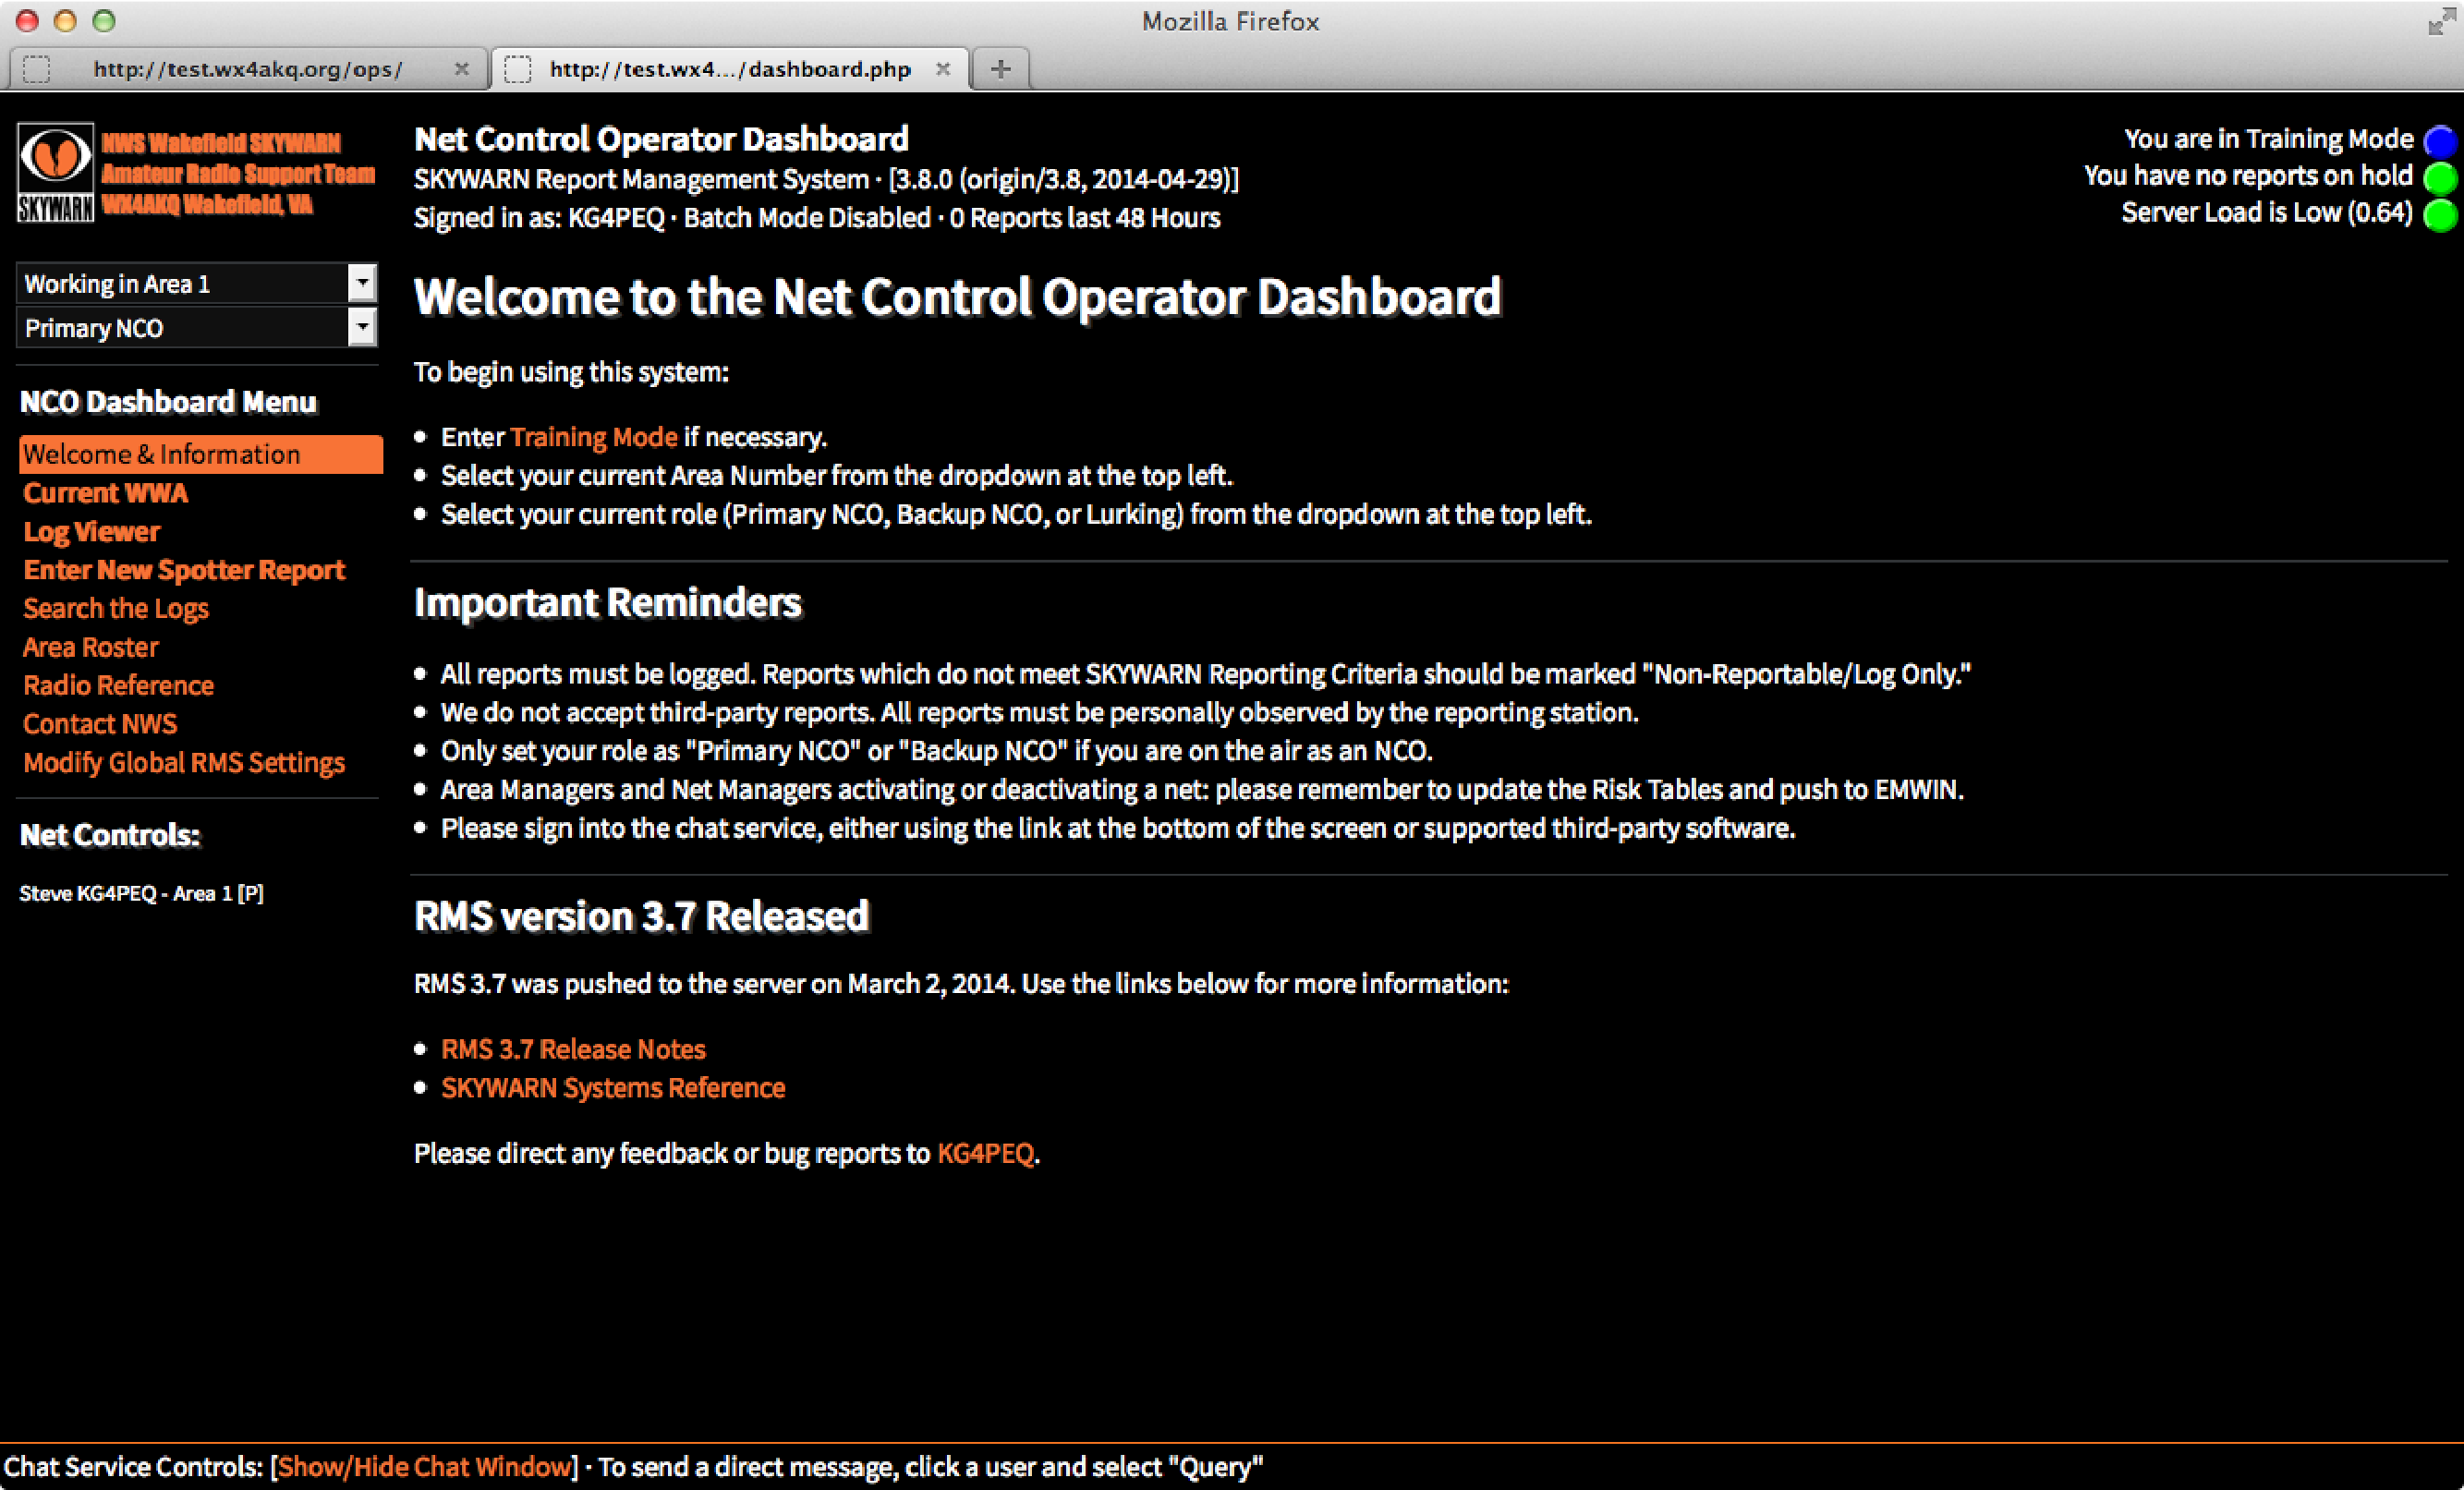
\includegraphics[width=\textwidth,keepaspectratio=true]{img/dash-main-screen}
  \caption{Initial view of the NCO Dashboard (in Training Mode).\label{fig:dash-main-screen}}
\end{figure}

%%%%%%%%%%%%%%%%%%%%%%%%%%%%%%%%%%%%%%%%%%%%%%%%%%%%%%%%%%%%%%%%%%%%%%%%

\section{Navigating NCO Dashboard}

As shown in Figure \ref{fig:dash-main-screen}, there are five main panels in NCO Dashboard:

\begin{itemize}
\item \textbf{Status Bar.} The Status Bar is located across the top of the screen and indicates the current system version, current user, Batch Mode status, and systemwide report count.
\item \textbf{RMS Status.}  The colored box at the top right corner shows the current RMS operating mode:  Online, Offline, or Training Mode.  It also provides a link to toggle Training Mode on and off.
\item \textbf{Menu Bar.}  The Menu Bar runs down the left side of the screen.  In addition to links to all NCO Dashboard functions, there is also a dropdown menu to indicate the current SKYWARN Operating Area.
\item \textbf{Main Window.}  The remainder of the screen will display the various NCO Dashboard functions, such as the Log Viewer and Current WWA.
\item \textbf{Chat Window.}  A web-based chat application is displayed at the bottom of the screen for easy communication with other team members.
\end{itemize}

The following functions are available in the NCO Dashboard and can be accessed via the Menu Bar down the left side of the screen:

\begin{itemize}
\item \textbf{\nameref{dash-current-wwa}.}  Displays current Watch, Warning, and Advisory (WWA) products for the current SKYWARN Operating Area.
\item \textbf{\nameref{dash-log-viewer}.}  Access pending, held, and completed net logs.
\item \textbf{\nameref{dash-new-report}.}  Create a new report or a follow-up for an existing report.
\item \textbf{\nameref{dash-search-logs}.}  Search pending, held, and completed net logs by call sign and/or date.
\item \textbf{\nameref{dash-area-roster}.}  Display a portion of the Team Roster for the current SKYWARN Operating Area.
\item \textbf{\nameref{dash-radio-ref}.}  Display SKYWARN frequencies and confidential repeater information for the current SKYWARN Operating Area.
\item \textbf{\nameref{dash-send-email}.}  Send a free-form text message to NWS Wakefield or a surrounding office.
\item \textbf{\nameref{dash-rms-settings}.}  Leadership Team members can modify various RMS settings.
\end{itemize}

The Menu Bar also contains a list of other Net Control Operators and their current role (primary/backup Net Control).

%%%%%%%%%%%%%%%%%%%%%%%%%%%%%%%%%%%%%%%%%%%%%%%%%%%%%%%%%%%%%%%%%%%%%%%%

\section{Setting Current Area}\label{dash-set-area}

Upon accessing the NCO Dashboard for the first time, use the dropdown menu in the top left corner to select your current SKYWARN Operating Area.  This setting controls several functions of the NCO Dashboard:

\begin{itemize}
\item Specifies which Operating Area is used for the display of the \nameref{dash-current-wwa}, \nameref{dash-area-roster}, and \nameref{dash-radio-ref} functions.
\item Sets the default Operating Area selected when using the \nameref{dash-new-report} function.
\item Updates the Operating Area displayed to other users in the NCO Dashboard.
\end{itemize}

You will default to Area 1 (Richmond) on the very first login, but after selecting a new area, this setting will be retained between logins.

%%%%%%%%%%%%%%%%%%%%%%%%%%%%%%%%%%%%%%%%%%%%%%%%%%%%%%%%%%%%%%%%%%%%%%%%

\section{Setting Current Role}\label{dash-set-role}

In addition to \nameref{dash-set-role}, you will need to select your role each time you access the NCO Dashboard.  This makes it much easier for remote team members to determine which NCO's are performing which Net Control function.

\begin{itemize}
\item {\bf Primary NCO} or {\bf Backup NCO}.  If the user is officially engaged in the operation of a net, one of these two roles should be selected.
\item {\bf Lurker}.  This option should be selected by users who want to be able to watch the net logs and chat, but who are not actively involved in the operation of a net.
\end{itemize}

Lurkers do not appear in the list of current Net Controls displayed in the Dashboard.

%%%%%%%%%%%%%%%%%%%%%%%%%%%%%%%%%%%%%%%%%%%%%%%%%%%%%%%%%%%%%%%%%%%%%%%%

\section{Entering Training Mode}\label{enter-training-mode}

The NCO Dashboard is equipped with a fully functional Training Mode which allows Net Control Operators to practice the use of the system without sending reports to the National Weather Service.

Reports created in Training Mode are submitted to a separate training log.

To enter Training Mode, use the link in the upper right corner of the screen.  While in Training Mode, you will see a blue box in the top right corner which says, ``Training Mode Enabled.''  Remember to exit Training Mode when you are done.  Your Training Mode status will be remembered between sessions on the same computer, and you do not want to inadvertently log ``live'' reports in Training Mode!

%%%%%%%%%%%%%%%%%%%%%%%%%%%%%%%%%%%%%%%%%%%%%%%%%%%%%%%%%%%%%%%%%%%%%%%%

\section{Viewing Current Net Controls}\label{dash-view-users}

A list of other users who are signed in to the NCO Dashboard \emph{and} who have selected either Primary or Backup NCO as their current role will be displayed along with their selected SKYWARN Operating Area.  This list will appear below the list of options in the Menu Bar.

Like most of the information in the NCO Dashboard, this user list updates automatically every few seconds.

For more information on roles, see \nameref{dash-set-role} on page \pageref{dash-set-role}.

%%%%%%%%%%%%%%%%%%%%%%%%%%%%%%%%%%%%%%%%%%%%%%%%%%%%%%%%%%%%%%%%%%%%%%%%

\section{Current WWA}\label{dash-current-wwa}

A list of current Watches, Warnings, and Advisories (WWA) for your current SKYWARN Operating Area can be displayed at any time by clicking the \emph{Current WWA} link in the Menu Bar.  See \nameref{dash-set-area} for information on selecting your current SKYWARN Operating Area.

The initial view, shown in Figure \ref{fig:dash-wwa-list}, shows the type of WWA, counties/cities, issue date, and issue time.

\begin{figure}[t]
  \centering
  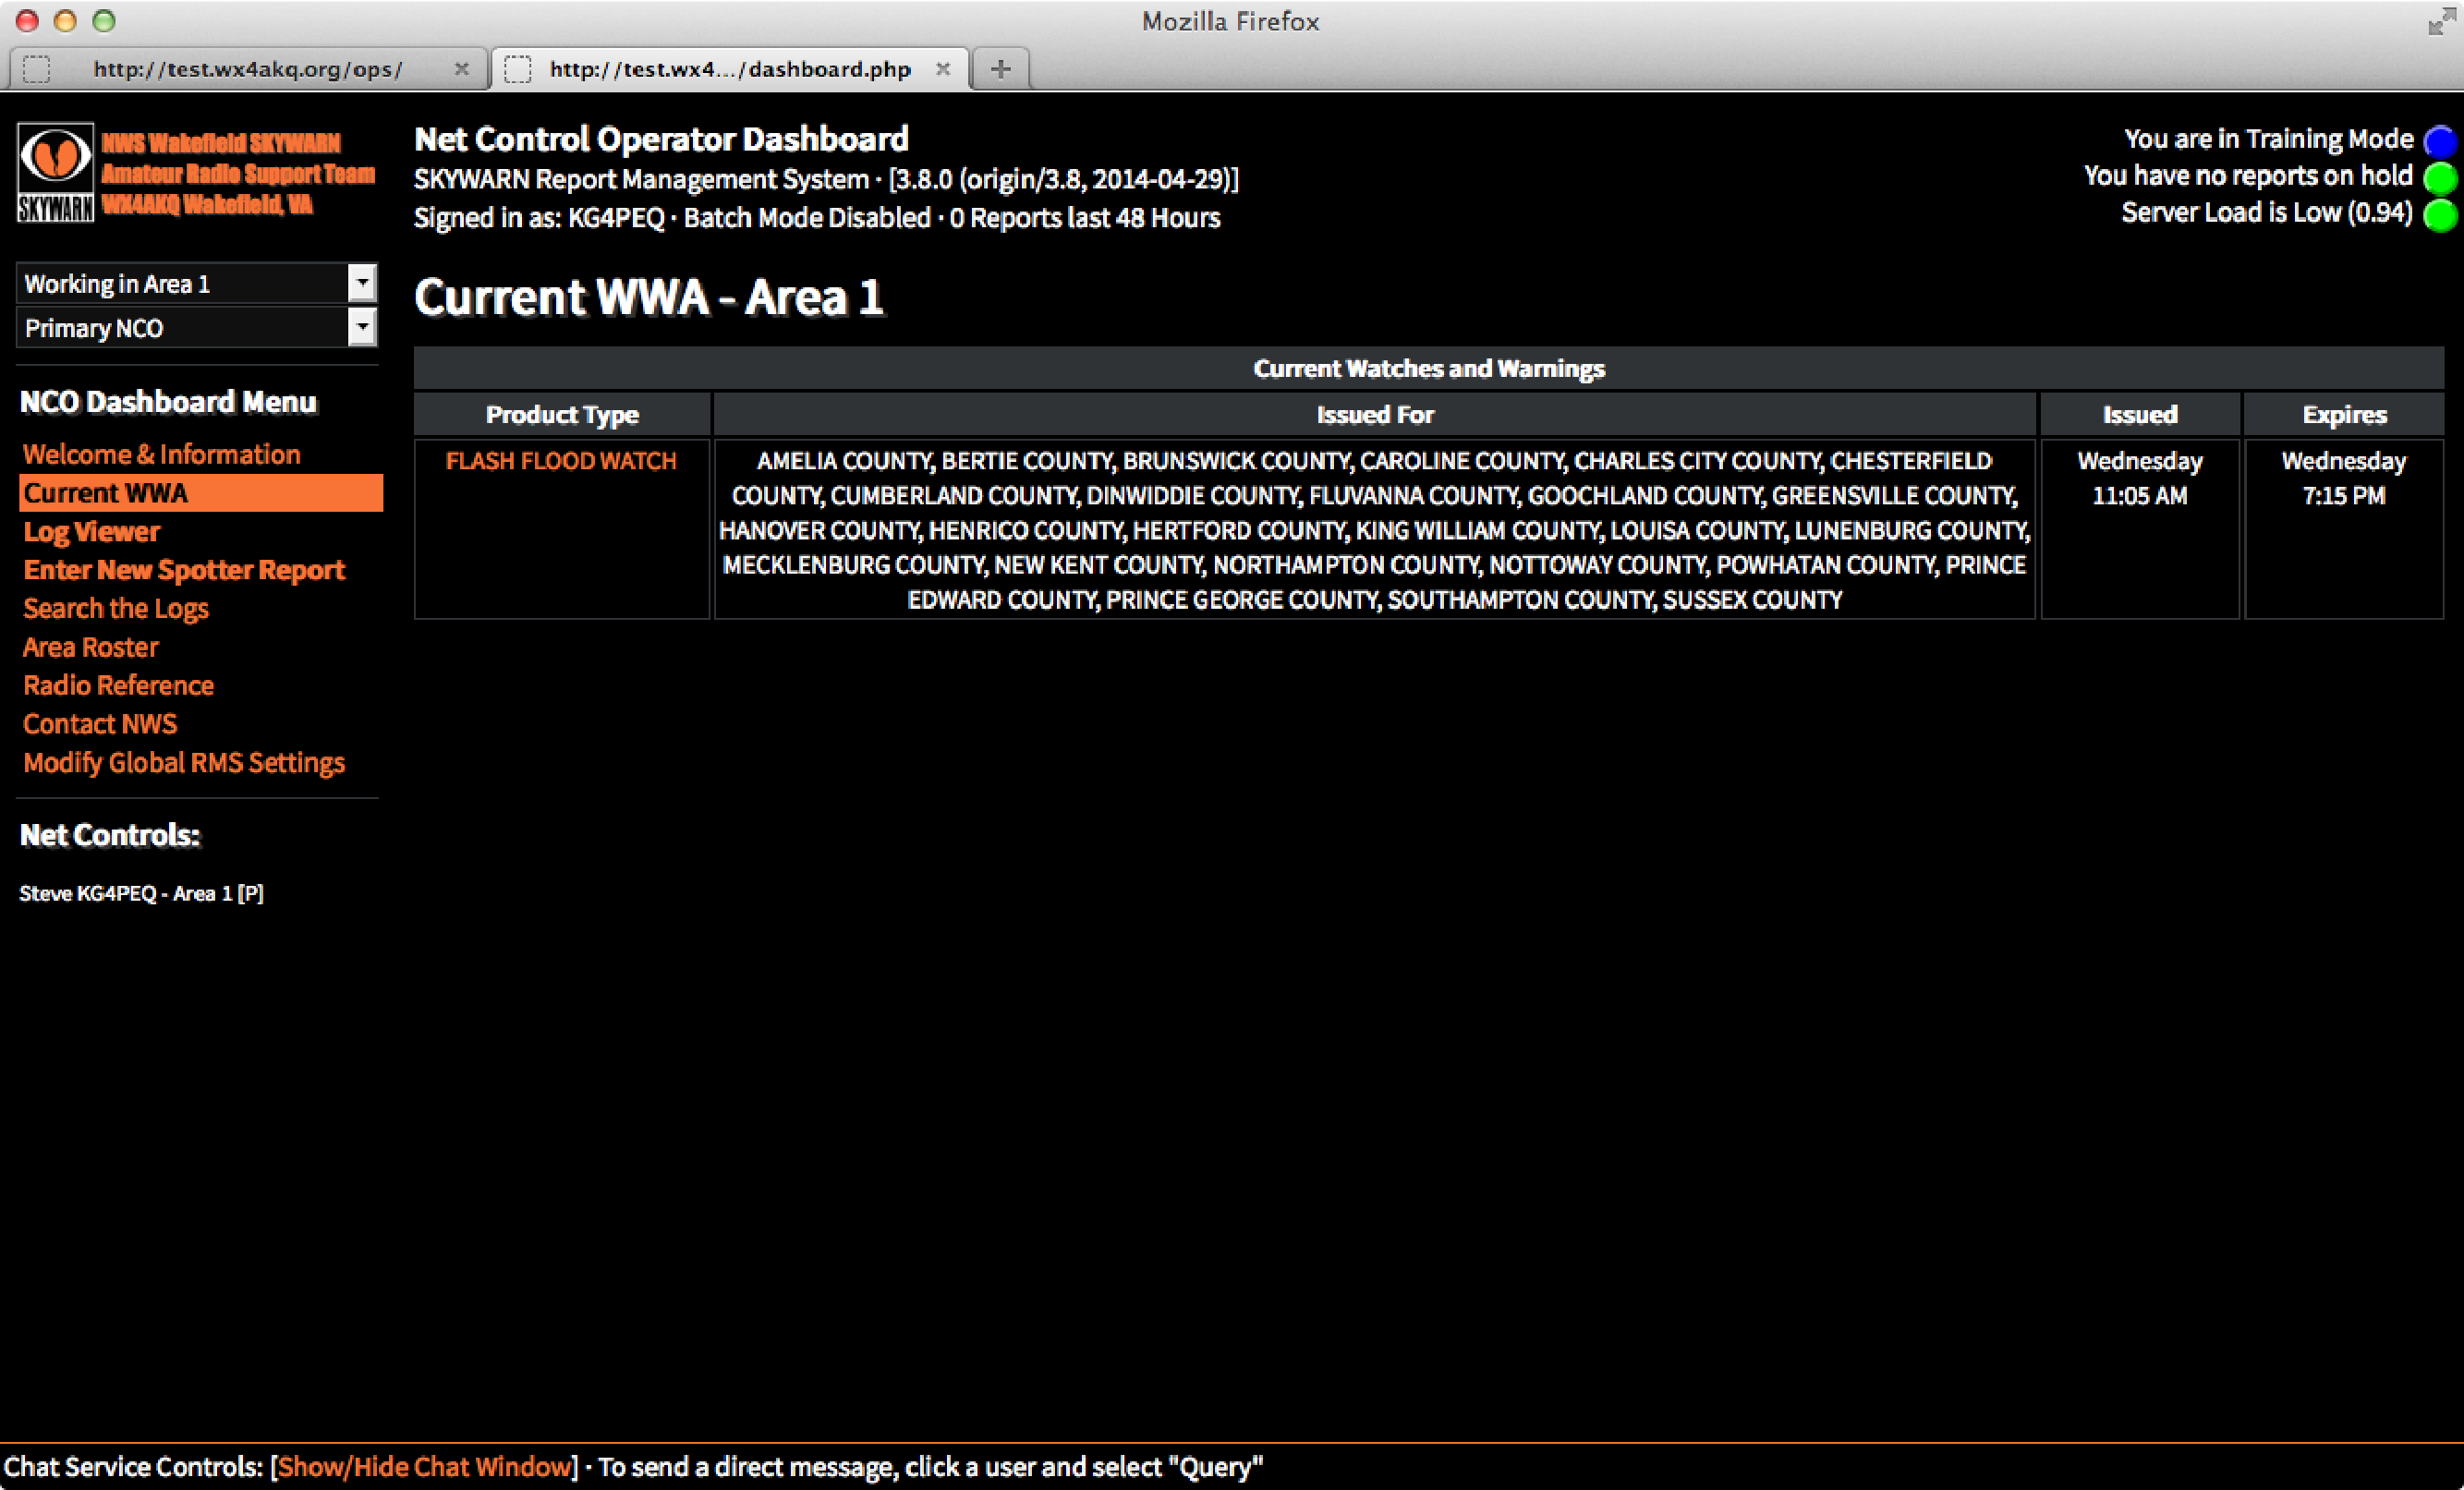
\includegraphics[width=\textwidth,keepaspectratio=true]{img/dash-wwa-list}
  \caption{List of current Watches, Warnings, and Advisories (WWA) as viewed in the NCO Dashboard.\label{fig:dash-wwa-list}}
\end{figure}

To view the full text of the WWA, click on the orange text in the \emph{Product Type} column.  The text is displayed on the screen, as shown in Figure \ref{fig:dash-wwa-item}.

\begin{figure}[t]
  \centering
  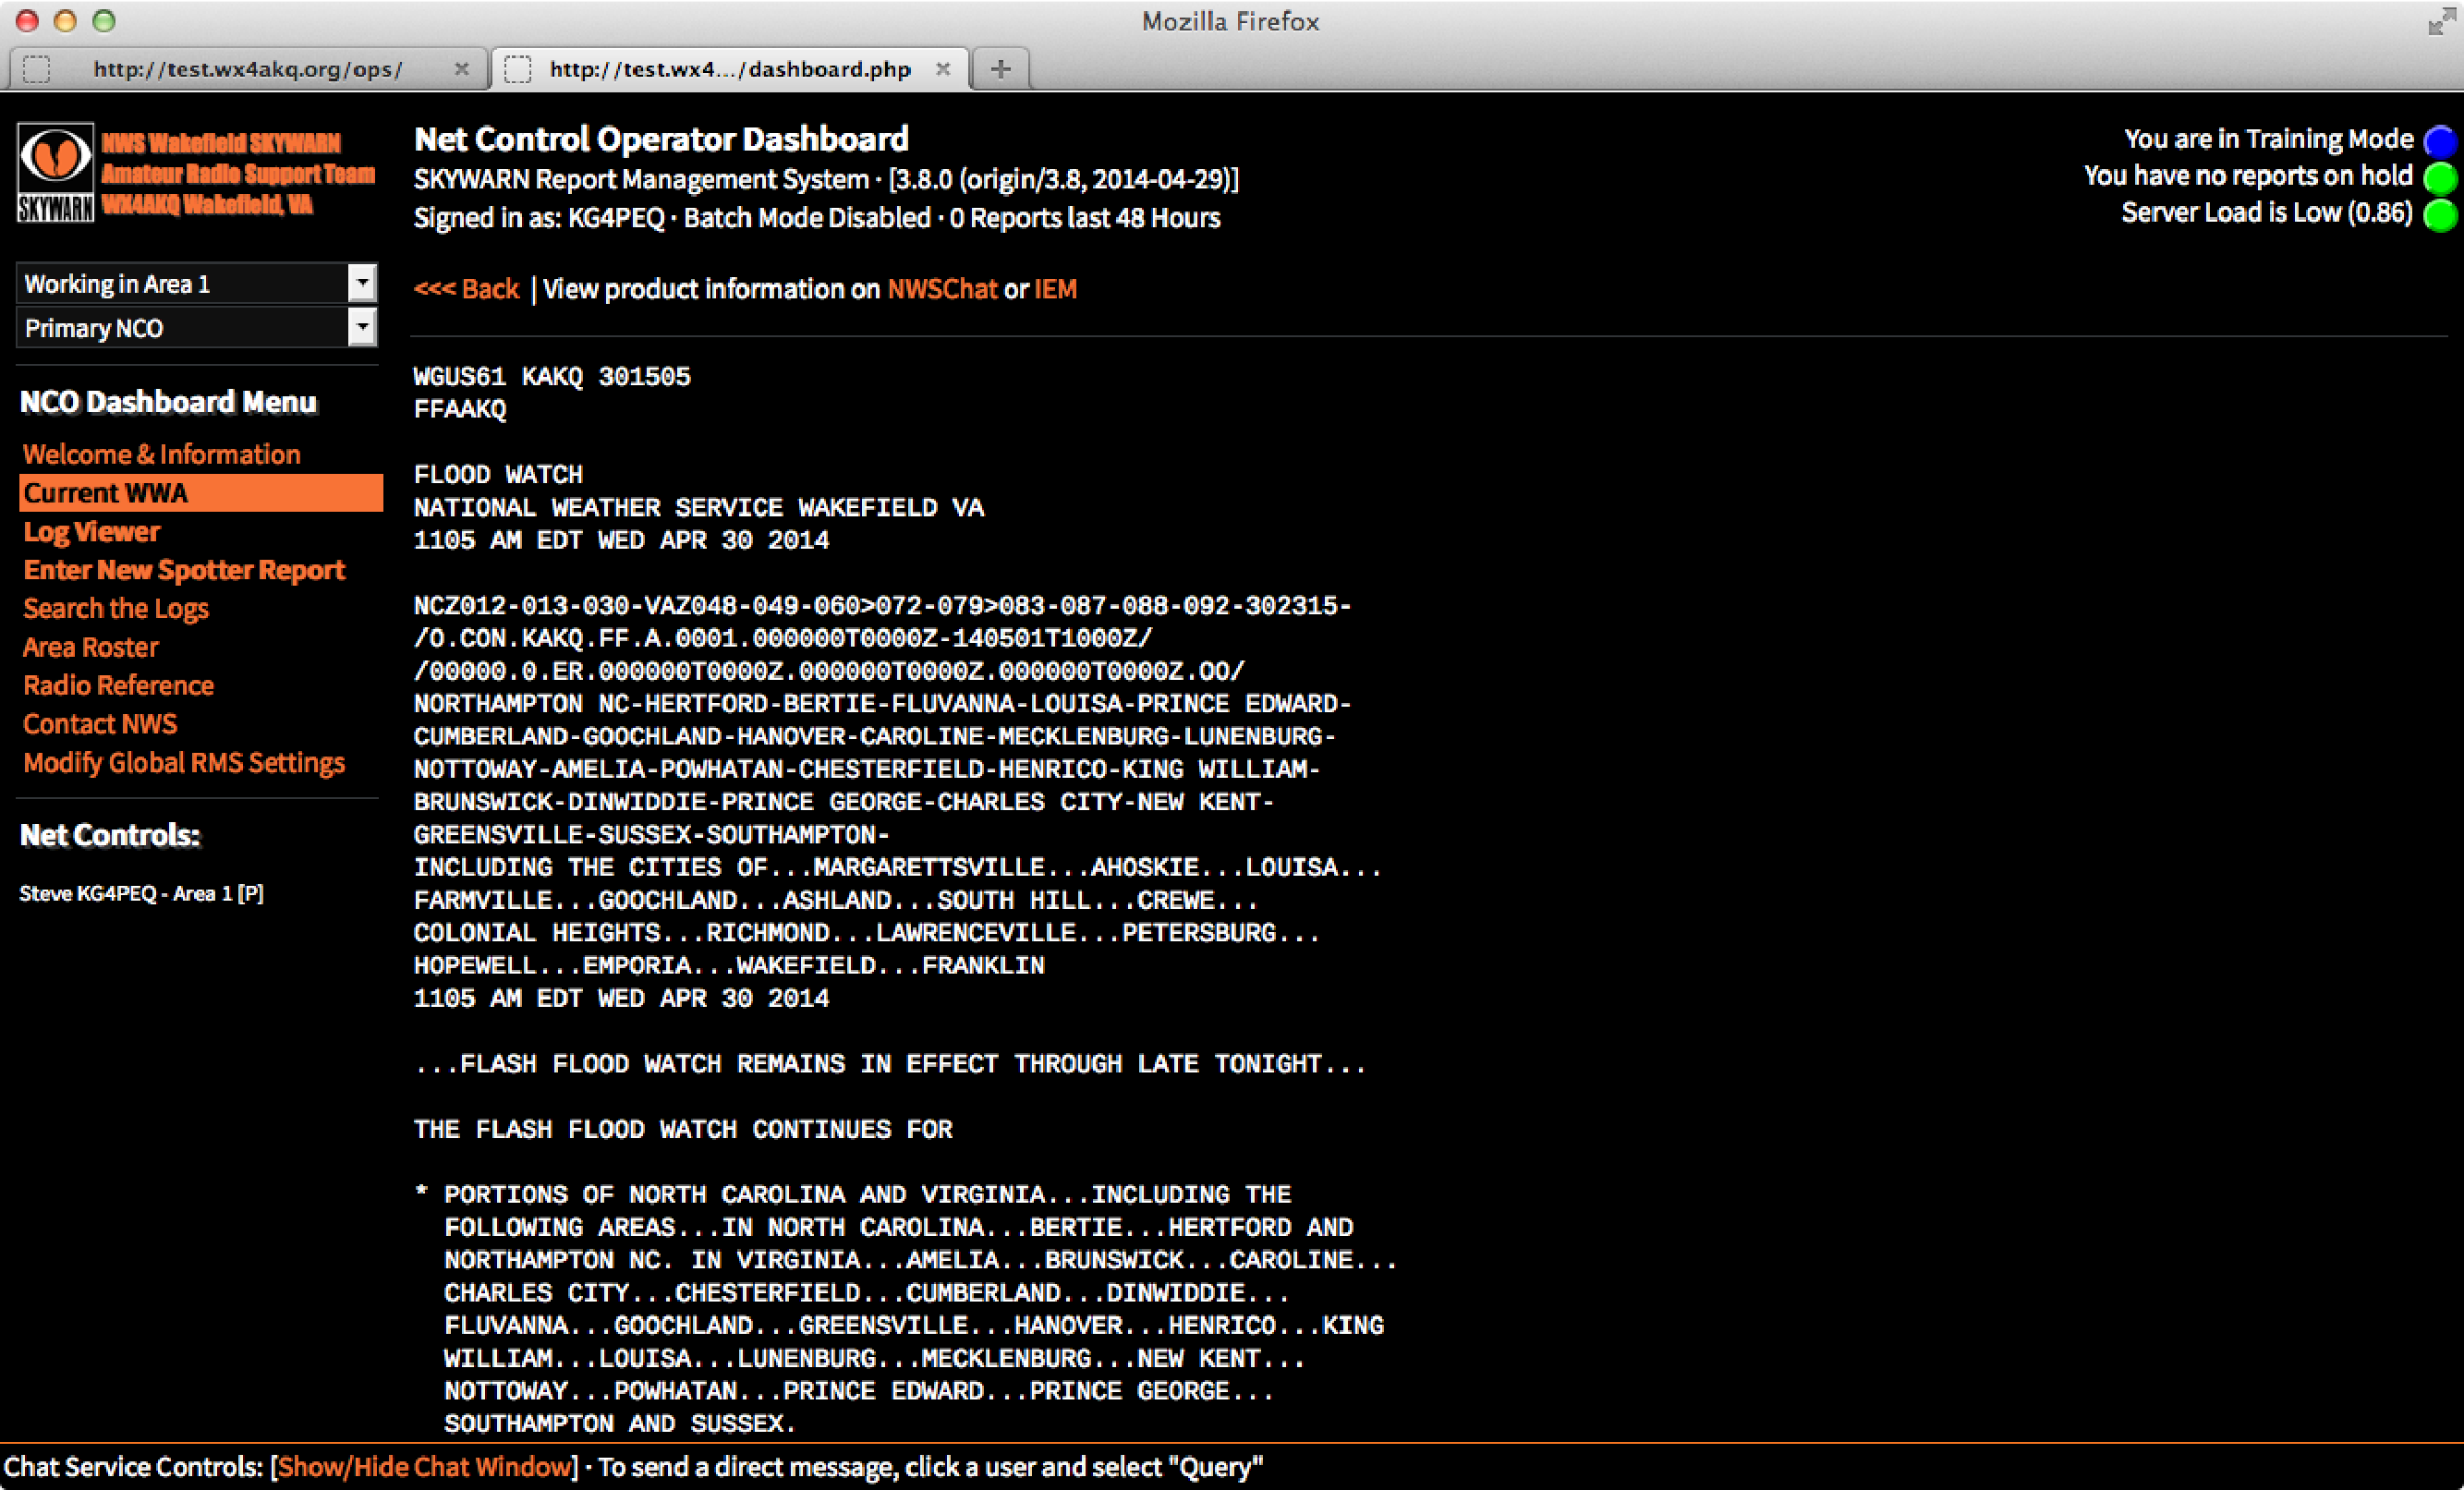
\includegraphics[width=\textwidth,keepaspectratio=true]{img/dash-wwa-item}
  \caption{WWA item text view.\label{fig:dash-wwa-item}}
\end{figure}

%%%%%%%%%%%%%%%%%%%%%%%%%%%%%%%%%%%%%%%%%%%%%%%%%%%%%%%%%%%%%%%%%%%%%%%%

\section{NWSChat and IEM Integration}\label{iem-integration}

When viewing the product text, you will notice that some products include links to view information in NWSChat and IEM.  These links are visible in Figure \ref{fig:dash-wwa-item}.

NWSChat and IEM are two similar systems which aggregate warning related data including radar imagery, warning outlines, and Spotter reports.

Both systems receive data at about the same time, though in some cases, one may be more up-to-date or have a more complete set of data than the other, so we provide links to both.

\orangebox{Pro Tip}{NWSChat and IEM are great tools for viewing the outline of warnings on top of current and historical radar imagery.  Spotter reports are frequently only visible on IEM, and will only appear once the reports are published in a Local Storm Report (LSR).\\\\With regard to mapping of warning polygons, both NWSChat and IEM provide excellent web-based alternatives to popular applications such as GRLevel3, WeatherTAP, and Radarscope, when these other software packages are not available or are not convenient.}  

An IEM view of a Severe Thunderstorm Warning can be seen in Figure \ref{fig:dash-emwin-iembot}.

\begin{figure}[t]
  \centering
  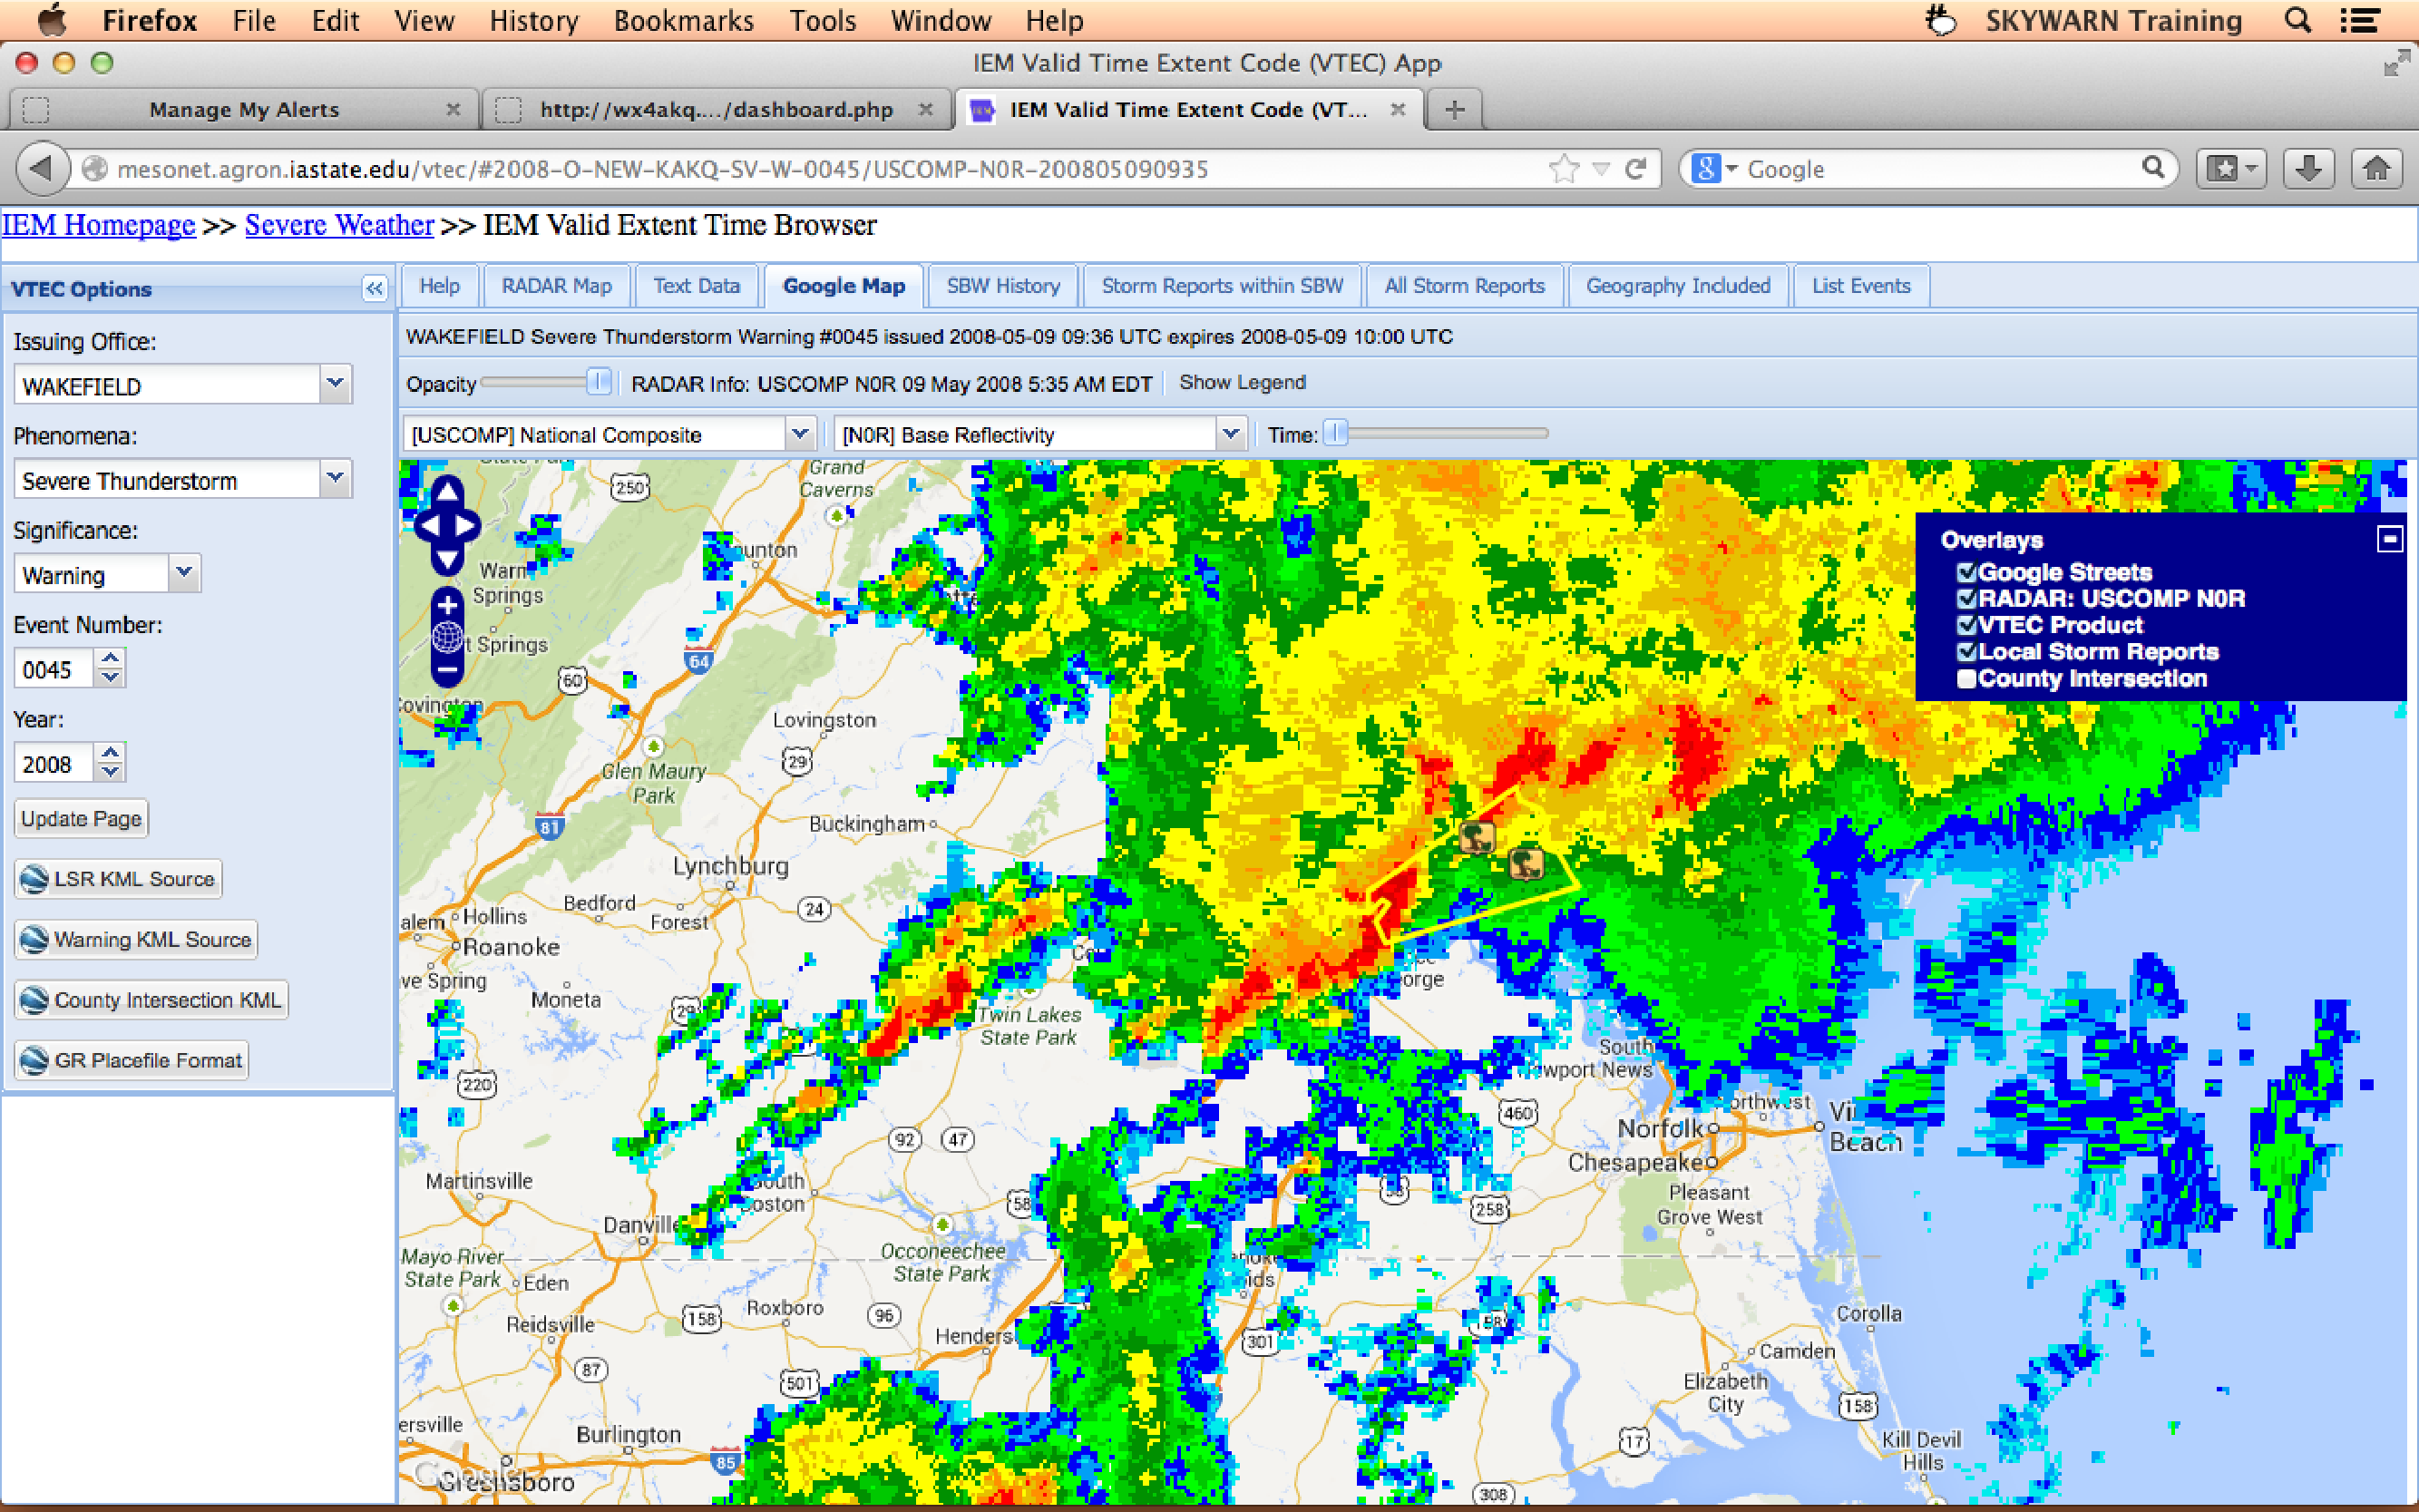
\includegraphics[width=\textwidth,keepaspectratio=true]{img/dash-emwin-iembot-1}
  \caption{IEM view of a Severe Thunderstorm Warning, showing the Storm Based Warning (SBW) polygon over the initial radar imagery.  Tabs near the top of the screen provide access to other information about the warning, including Spotter reports.\label{fig:dash-emwin-iembot}}
\end{figure}

It is \textbf{not} necessary for most SKYWARN Net Control Operators to be intimately familiar with the operation of NWSChat or IEM.  However, it is good to be aware that the tools exist.

Sometimes a Spotter may want to know if their community is within a warning polygon, and the mapping functionality of NWSChat and IEM could be handy for determining that information.

%%%%%%%%%%%%%%%%%%%%%%%%%%%%%%%%%%%%%%%%%%%%%%%%%%%%%%%%%%%%%%%%%%%%%%%%

\section{Log Viewer}\label{dash-log-viewer}

The Log Viewer displays pending, held, and completed logs based on the filter settings.  The default view, seen in Figure \ref{fig:dash-log-view}, shows any reports in the queue, waiting to be released from the system.

\begin{figure}[h]
  \centering
  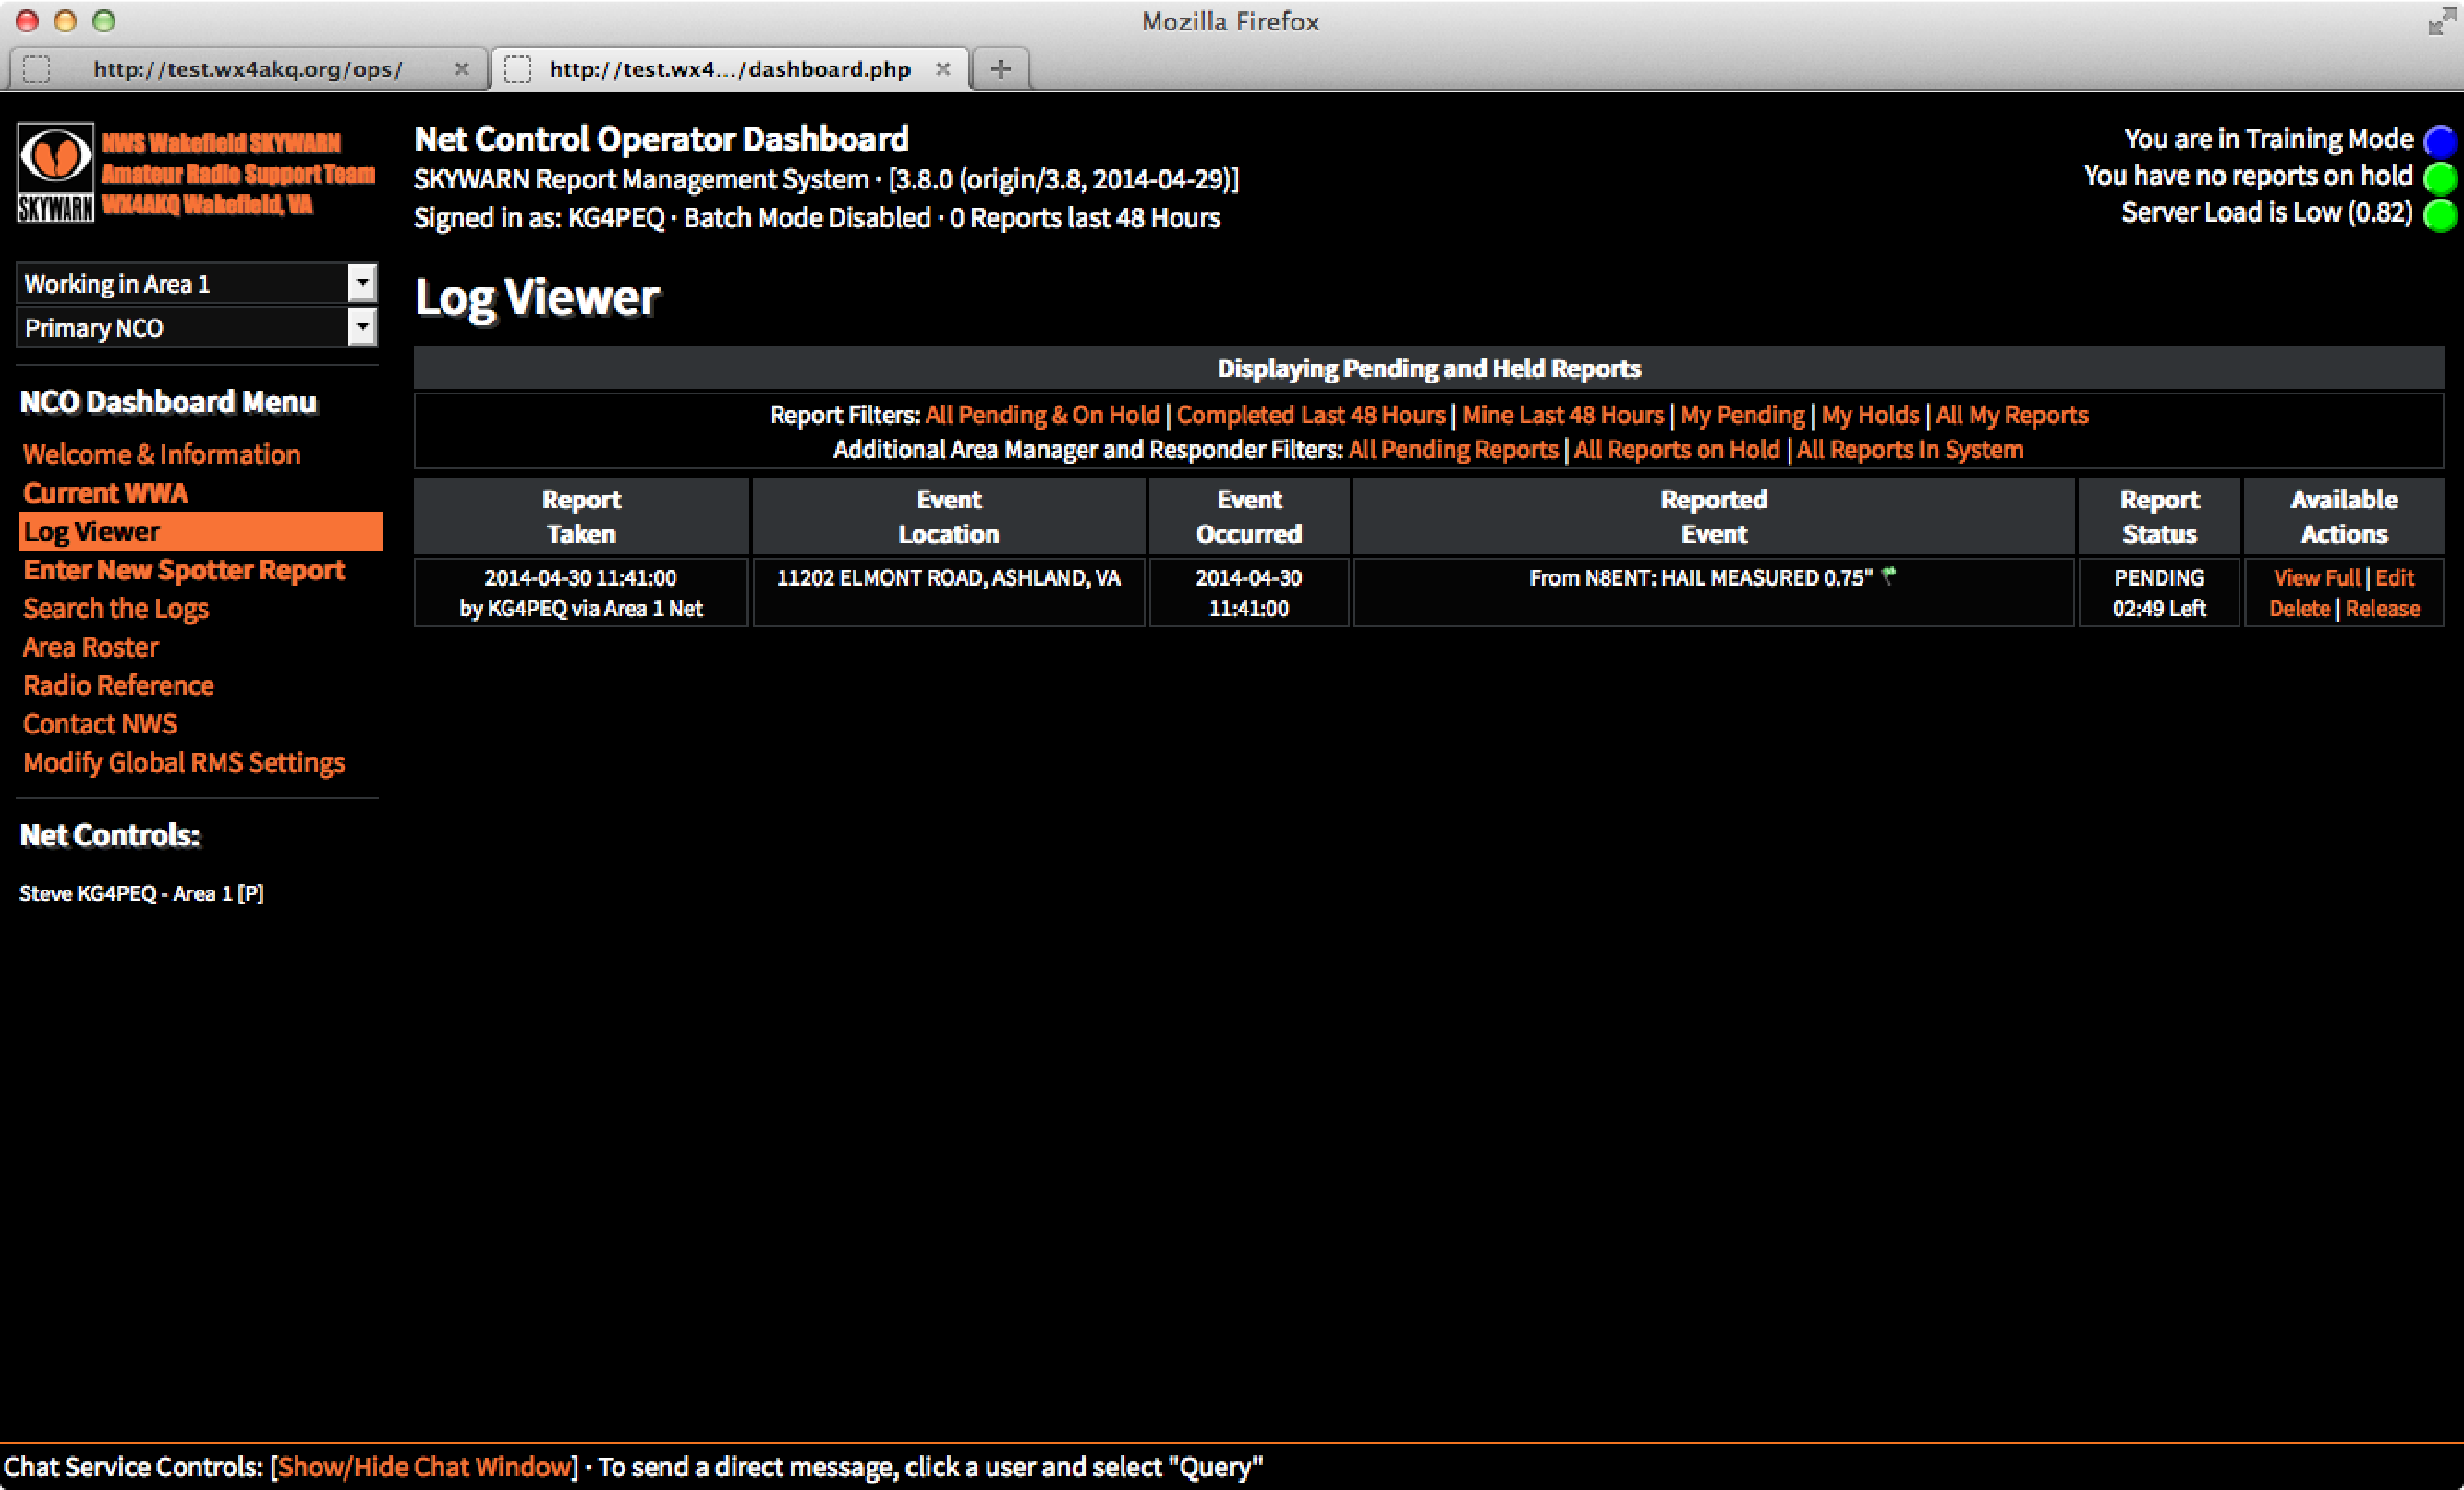
\includegraphics[width=\textwidth,keepaspectratio=true]{img/dash-log-view-withreport}
  \caption{Default Log Viewer display, showing one report waiting to be released.\label{fig:dash-log-view}}
\end{figure}

\subsection{Report Status Codes}\label{dash-report-status-codes}

\nameref{rms} supports four different report status codes, which will be reflected in the Log Viewer:

\begin{itemize}
\item \textbf{Pending.}  Pending reports have been set to route to a \nameref{rms-offices} via electronic routing.  A timer will count down from the Release Delay specified in the RMS Settings.  See \nameref{dash-rms-settings} on page \pageref{dash-rms-settings} for information on the Release Delay.
\item \textbf{On Hold.}  A report can be placed in an ``On Hold'' status if additional information is needed from the Spotter, or for most any other reason.  A report which is On Hold will be held in the system indefinitely, and will not be marked as Complete or otherwise released from the system until the hold is removed.  Reports which are being edited are systematically placed into an On Hold condition to prevent automatic release during the editing process.
\item \textbf{Complete.}  Completed reports have either been marked as complete during the log entry process (for example, a report which was already relayed by telephone, e-mail, eSpotter, or direct radio contact), or have been systematically marked as complete during the electronic relay process.  Completed reports cannot be edited or deleted, but follow-up reports can be submitted.
\item \textbf{Log Only.}  Reports which do not meet reporting criteria should be set as ``Log Only'' during the report entry process.  These reports are not electronically relayed, and may be edited or deleted at any time.
\end{itemize}

\subsection{Log Viewer Layout and Filters}\label{log-layout-filters}

As seen in Figure \ref{fig:dash-log-view}, the Log Viewer has six columns:

\begin{itemize}
\item \textbf{Report Taken.}  Shows the date and time the report was collected.
\item \textbf{Event Location.}  The location of the event as reported by the Spotter.
\item \textbf{Event Occurred.}  The event date and time collected from the Spotter.
\item \textbf{Reported Event.}  The details of the severe weather event.  A green or red flag icon appears next to each report.  A red flag indicates the report has been flagged as a suspicious report.
\item \textbf{Report Status.}  Shows the \nameref{dash-report-status-codes} of each report.  In the case of pending reports, the time left to edit the report shows under the status.
\item \textbf{Available Actions.}  Links to View, Edit, Delete, and Release reports, as appropriate based on access class and report status.
\end{itemize}

\orangebox{Available Action Permissions}{The links enabled in the \emph{Available Actions} column of the Log Viewer are determined by both report status and your user access class.\\\\Completed reports cannot be edited or deleted by anyone.\\\\Net Control Operators may edit, delete, or manually release their own reports, but not those taken by other NCO's.\\\\SKYWARN Leadership Team members have the ability to edit, delete, and manually release reports taken by anyone, at least until the report is released from the system and marked as Complete.}

In the case of Pending reports, there will often be a brief period, up to one minute, between the time the countdown timer reaches zero and when the report is actually released from the system.  This is because a server-side script runs once each minute to handle the release of reports from the system.  When the timer reaches zero, the timer will disappear from the Log Viewer.  There is no Net Control action required, though, and the report will auto-release the next time the script runs on the server.

You can change the reports shown in the Log Viewer by applying filters.  There are a number of different filter settings available:

\begin{itemize}
\item \textbf{All Pending \& On Hold.}  This is the default.  Shows all reports which are either held or pending release, from all areas.
\item \textbf{Completed Last 48 Hours.}  Shows all reports from all areas completed over the past 48 hours.
\item \textbf{Mine Last 48 Hours.}  Shows all reports submitted by the current NCO during the past 48 hours.
\item \textbf{My Pending.}  Shows all pending reports for the current NCO.
\item \textbf{My Holds.}  Shows all held reports for the current NCO.
\item \textbf{All My Reports.}  Shows all reports submitted by the current NCO since the beginning of time.
\end{itemize}

SKYWARN Responders and Leadership Team members have additional filter options available, which are shown in Figure \ref{fig:dash-log-view} on page \pageref{fig:dash-log-view}.

\subsection{View a Report}

To view a report, click on the \textbf{View Full} link in the far right column.  The details of the report, including time stamp, location, report text, routing and status information will be displayed on the screen, as shown in Figure \ref{fig:dash-report-view}.

\begin{figure}[h]
  \centering
  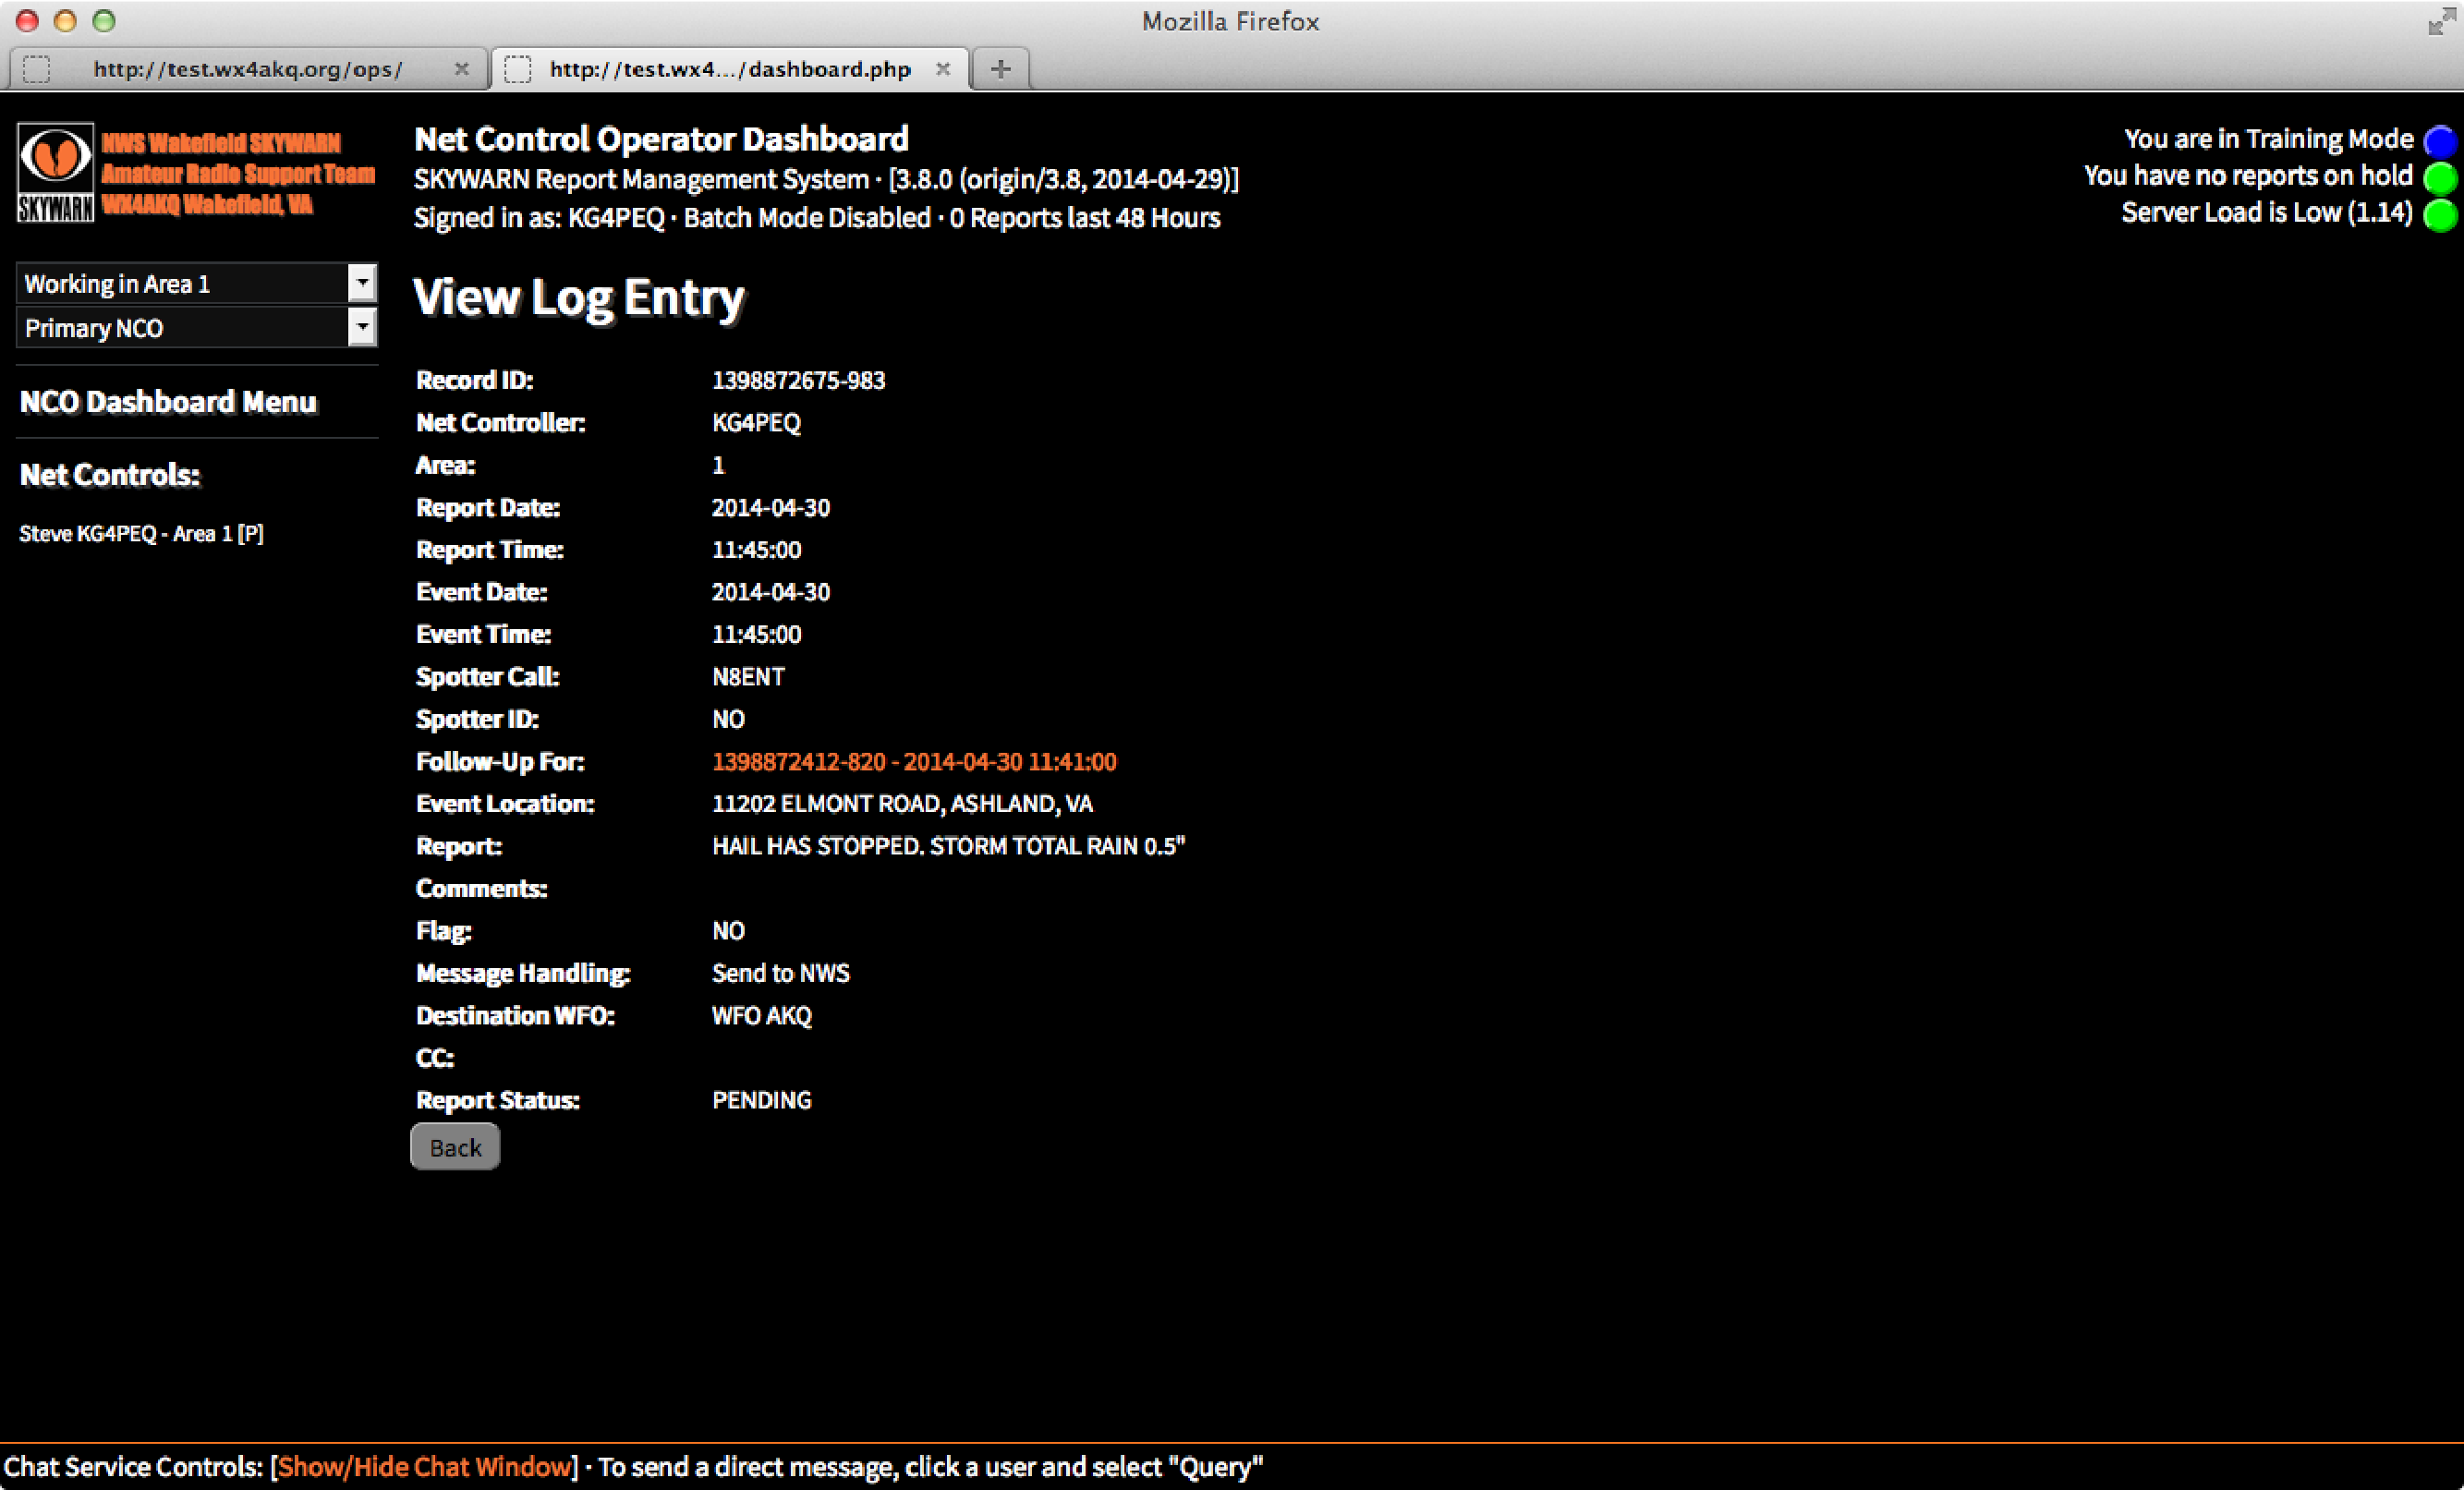
\includegraphics[width=\textwidth,keepaspectratio=true]{img/dash-report-view}
  \caption{Report View, showing the details of a pending report.\label{fig:dash-report-view}}
\end{figure}

\subsection{Edit a Report}

The \textbf{Edit} option, when available, allows you to edit one of your reports, as long as that report has not yet been released from the system.  When you click \textbf{Edit}, the report is automatically placed into ``On Hold'' status so it will not be released, even if the timer for the report is about to expire.

Once you have completed your edits, you will submit the report back to the queue and the countdown timer will start again.

\subsection{Delete a Report}

Any report you have taken which has not yet been released from the system can be deleted using the \textbf{Delete} link.  You will be asked to confirm this action.  Deleting a report is permanent;  there is no way to retrieve a report once it has been deleted.

\subsection{Manually Release a Report}\label{manual-release}

On rare occasions it may be necessary to circumvent the release countdown mechanism and force a report out of the system.  For example, an urgent report should be released while a phone call is made to the receiving WFO.  Or, a priority report might be released early while \nameref{rms-batch-mode} is active.

To release a Pending report, click on the \textbf{Release} link.  You will be asked to confirm the release.

\orangebox{Be Careful}{Avoid using the manual release function for routine reports.  Let the system do its job and release the reports automatically unless a report is truly urgent and needs to go right away.}

%%%%%%%%%%%%%%%%%%%%%%%%%%%%%%%%%%%%%%%%%%%%%%%%%%%%%%%%%%%%%%%%%%%%%%%%

\section{Enter New Spotter Report}\label{dash-new-report}

The process of entering a new Spotter report is very straightforward.  The NCO Dashboard provides a simple web form which allows for quick entry of date, time, identification, location, and report details, along with all required routing information.  Figure \ref{fig:dash-report-create} shows the Log Entry form as viewed in the NCO Dashboard.

\begin{figure}[h]
  \centering
  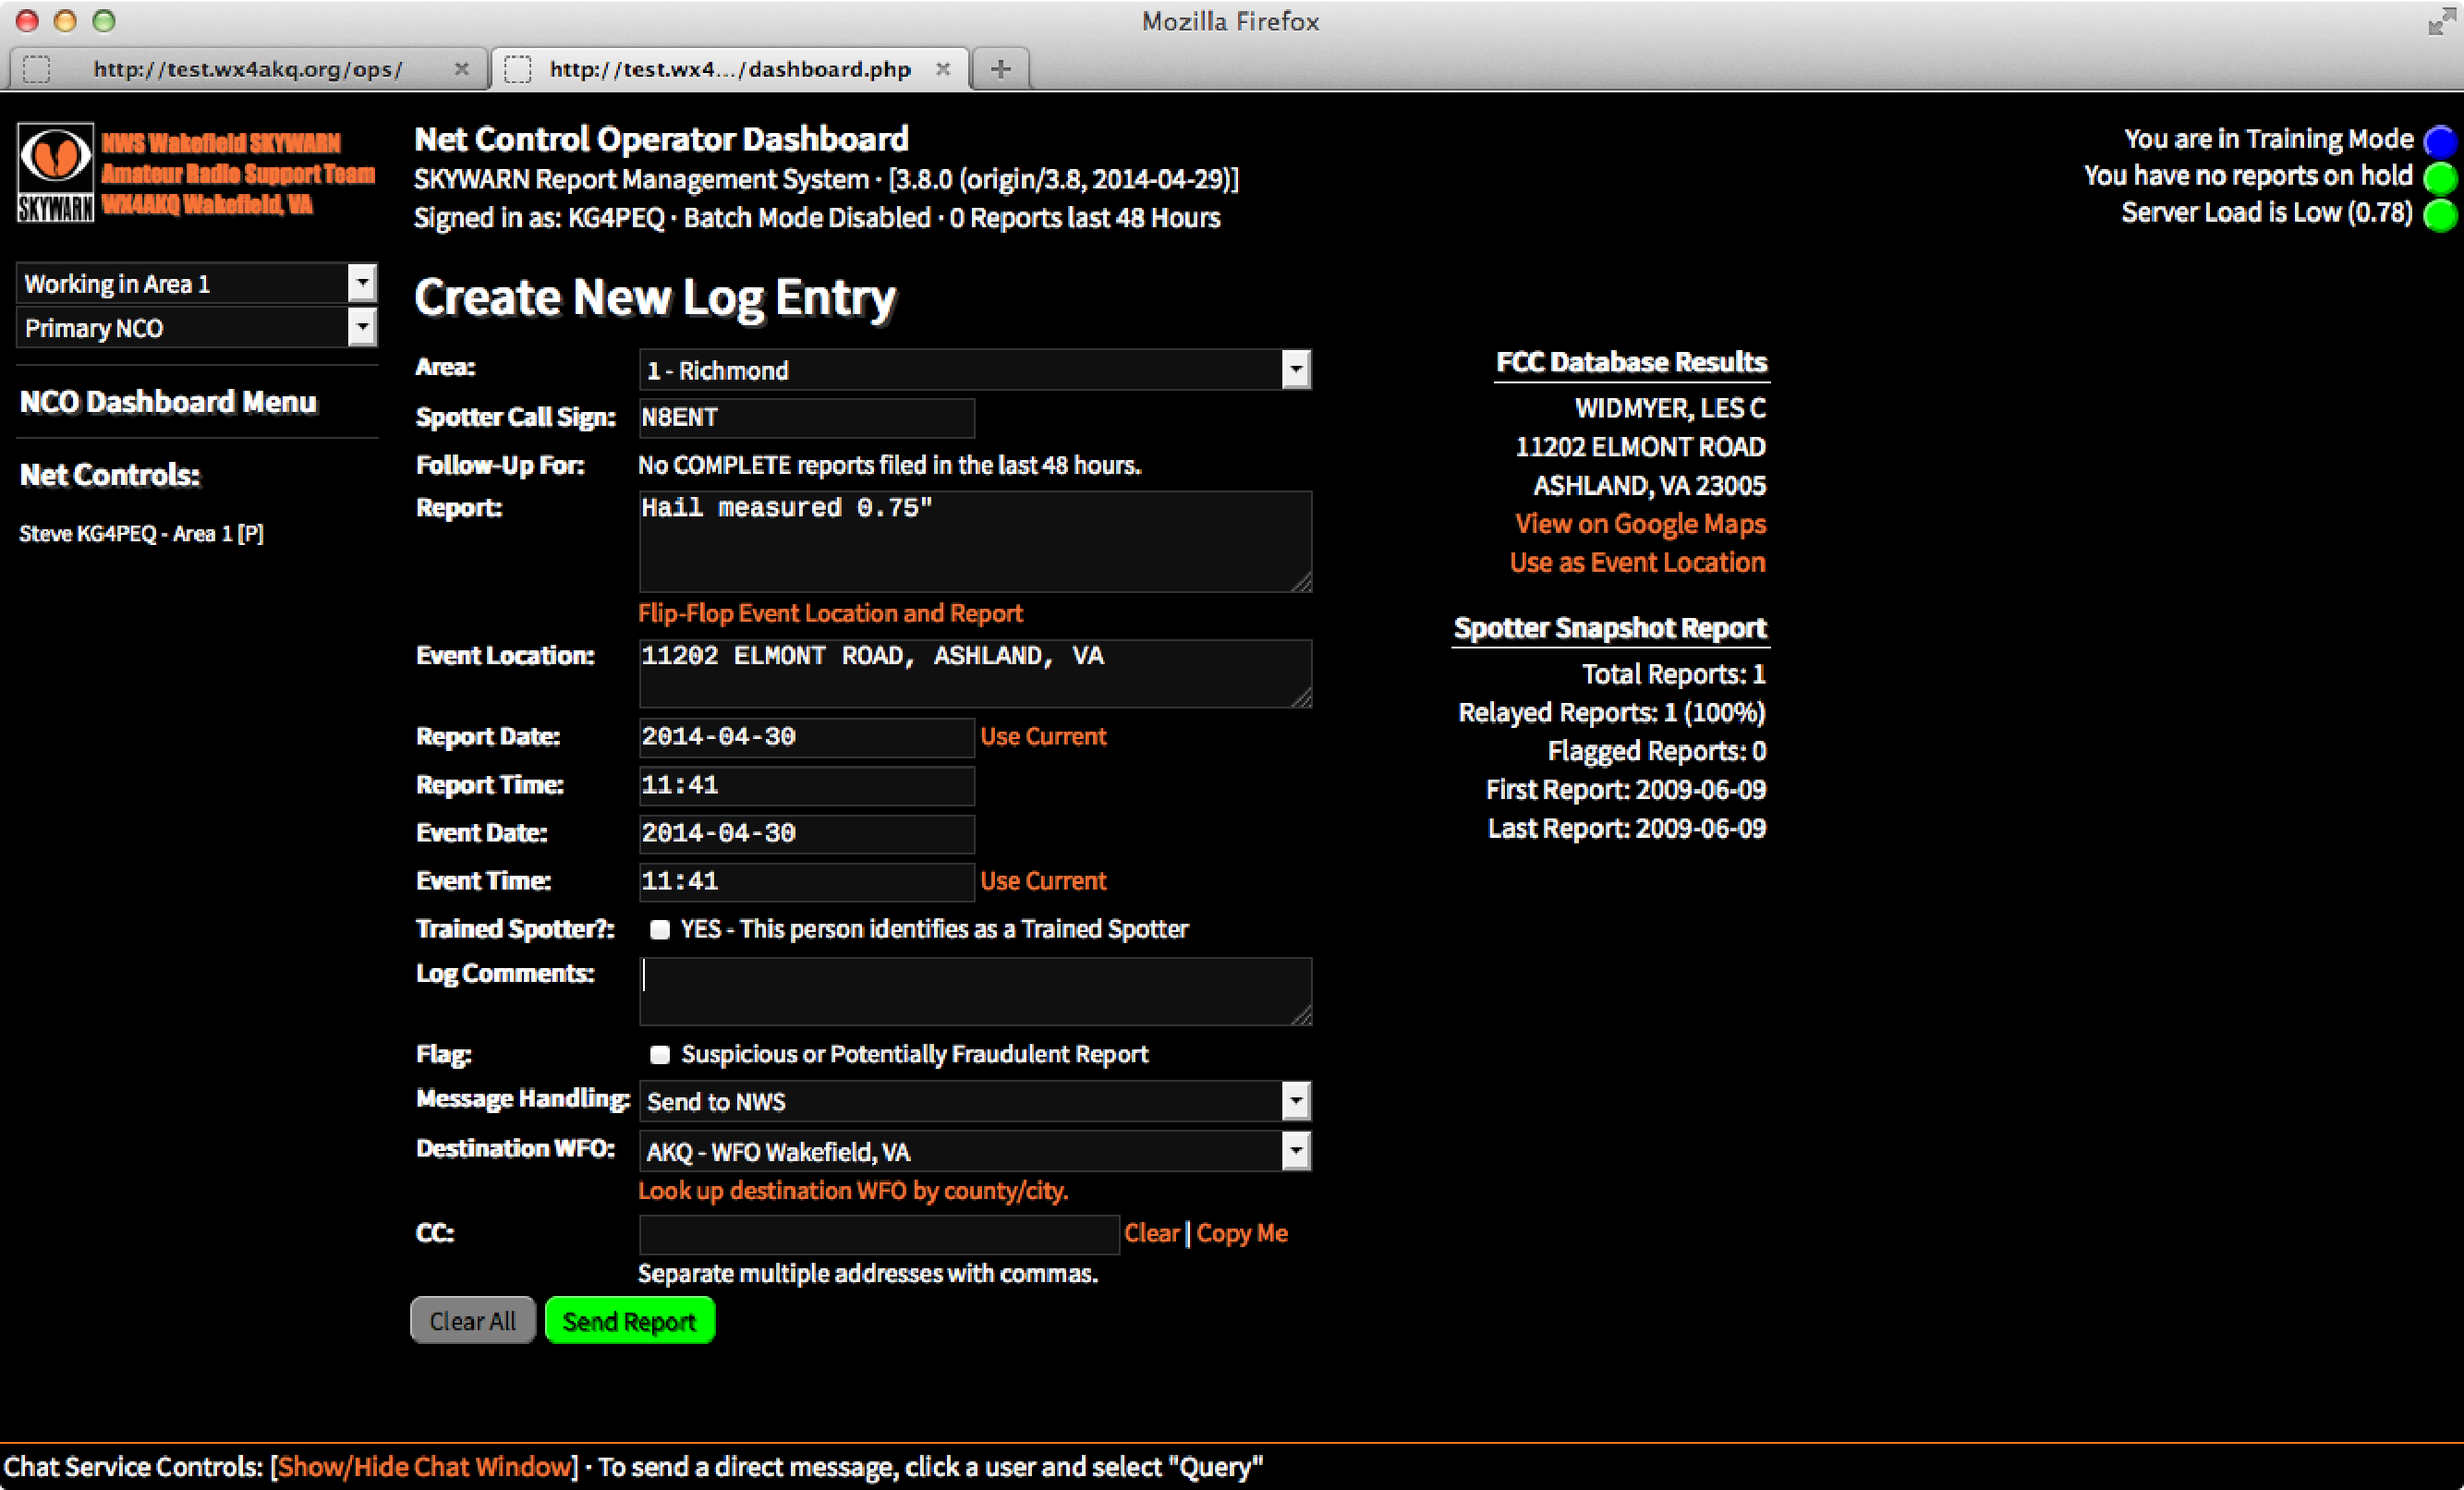
\includegraphics[width=\textwidth,keepaspectratio=true]{img/dash-report-create}
  \caption{The Log Entry form showing a Spotter report ready for submission.\label{fig:dash-report-create}}
\end{figure}

\subsection{Log Entry Fields}

There are four date and time fields on the Log Entry form:

\begin{itemize}
\item \textbf{Report Date} and \textbf{Report Time.}  This is the date and time the report is called in to the net.
\item \textbf{Event Date} and \textbf{Event Time.}  This is the date and time of the actual event, if known;  an estimate is okay.
\end{itemize}

When entering the date and time into these fields, formatting is not particularly important.  Here are some of the recognized formats:

\begin{itemize}
\item \verb|3/1/2013|
\item \verb|3-01-13|
\item \verb|March 1, 2013|
\item \verb|2:45 pm|
\item \verb|14:45|
\end{itemize}

For speed and convenience, there is a \textbf{Use Current} auto-fill link on the form, which will automatically complete the \emph{Report Date, Report Time,} and \emph{Event Date} fields.  A separate \textbf{Use Current} auto-fill link appears next to the \emph{Event Time} field.  You may manually complete the \emph{Event Time} field using information collected from the Spotter, or click the auto-fill link once you have confirmed the event is occurring ``right now.''

When you enter the Spotter's call sign, two pieces of magic happen.  First, the NCO Dashboard queries RMS for the Spotter's training status.  If the Spotter has reported to us that he/she is a Trained Spotter, then the \emph{Trained Spotter?} checkbox will automatically check itself.  The NCO Dashboard also queries RMS for any recently completed reports (within the last 48 hours) and provides a dropdown to file a Follow-Up Report.  For more information on Follow-Up reports, see \nameref{follow-up-reports} on page \pageref{follow-up-reports}.

If the \emph{Trained Spotter?} checkbox does not auto-check, you will need to ask the station if they are a trained Spotter.  If so, check the box, and the NCO Dashboard will pick up on their status on future reports.  If they are not trained, uncheck the box.

\orangebox{What about Spotter ID's?}{The National Weather Service stopped issuing Spotter ID's in 2012.  While some Spotters may still have a previously-issued Spotter ID, they are not required, and we do not collect them.  All we need to know is whether they are trained.}

Next, enter the location and the report details.

Remember, when entering the location:

\begin{itemize}
\item Be as specific as possible.
\item Actual street addresses are acceptable.
\item Cross-streets/nearest major intersection(s) are acceptable.
\item Nearby well-known landmarks are acceptable.
\item Position relative to a landmark or well-known community is acceptable;  for example, ``2 miles northeast of Ashland.''
\item Coordinates are acceptable, but \emph{only in decimal format}.
\item Do not simply enter ``home'' or ``QTH'' or a town/city name like ``Richmond.''
\end{itemize}

When entering the report details:

\begin{itemize}
\item Indicate whether the report is a measurement or an estimate.
\item Abbreviating (M) for ``measured'' and (E) for ``estimate'' is acceptable.
\item Review the report before submitting to ensure all possible details have been captured and recorded.
\end{itemize}

If the report is suspicious, check the \emph{Flag} box.  Refer to the \emph{SKYWARN Operations Manual} for information on determining and handling suspicious reports. 

\subsection{Message Handling Options}

The final fields on the Log Entry form are message handling options.

If a report meets the established reporting criteria, it should be sent to the National Weather Service.  Most of our reports will go to the Wakefield office, but some outlying areas may collect reports from Spotters in another area.  See \nameref{rms-offices} for a list of locations we can electronically submit reports to.

\orangebox{Not Sure?}{If you aren't sure which office a report should go to, you have a couple of options.  You can ask the Spotter which office serves their location (quite often, they will know), or you can send the report to your ``best guess.''  If it does go to the wrong office, it will be forwarded to the appropriate office by NWS employees, but this can delay report delivery.}

RMS supports message delivery via packet (actually, over the Winlink system), but for reports to Wakefield only.  The ``Copy WX4AKQ'' options in the message routing will work when transmitting reports to any WFO, but the reports will be sent to WX4AKQ via Winlink.

If a report has been relayed via radio or telephone and does not need to go electronically, there are routing options to accommodate that situation.

Possible routing options are:

\begin{itemize}
\item \textbf{Hold for Future Edit.}  This places the report into ``On Hold'' status.  You will need to come back to the report, set a routing option, and submit the report in order for it to go anywhere.
\item \textbf{Non Reportable/Log Only.}  For reports which do not meet reporting criteria.  This is also used to log emergency traffic which gets routed to police, fire, rescue, etc.
\item \textbf{Already Relayed to NWS.}  There are two options:  ``Phone'' and ``Direct to WX4AKQ.''  If a report was submitted via e-mail, e-Spotter, social media, or another method, just select ``Phone.''
\item \textbf{Send to NWS.}  The default routing.  Sends the message electronically to the selected WFO.
\item \textbf{Send to NWS, Copy WX4AKQ.}  Sends the message electronically to the selected WFO and sends a copy to WX4AKQ via Winlink.
\item \textbf{Send to WX4AKQ Only.}  Does not send to a WFO, but does send a copy to WX4AKQ via Winlink.
\end{itemize}

The \emph{CC:} field allows you to specify one or more e-mail addresses to receive a copy of the report.  Currently, this only works for reports which are set to relay to an NWS office.  If you would like to receive a copy via e-mail, click ``Copy Me.'' Add additional e-mail addresses separated by commas.

\subsection{Follow-Up Reports}\label{follow-up-reports}

Sometimes a Spotter will call back with an update to a previous report.  For example, they might report 1'' of snow, and then two hours later call back in with 2.5''.  In this case, since the second report is related to the first, you would want to enter this as a Follow-Up Report.

You may recall that the NCO Dashboard queries RMS for a 48-hour report history when you key a Spotter's call sign into the Log Entry form.  Any previous reports will appear in a dropdown menu next to \emph{Follow-Up For} in the Log Entry form, as shown in Figure \ref{fig:dash-followup-create}.

\begin{figure}[h]
  \centering
  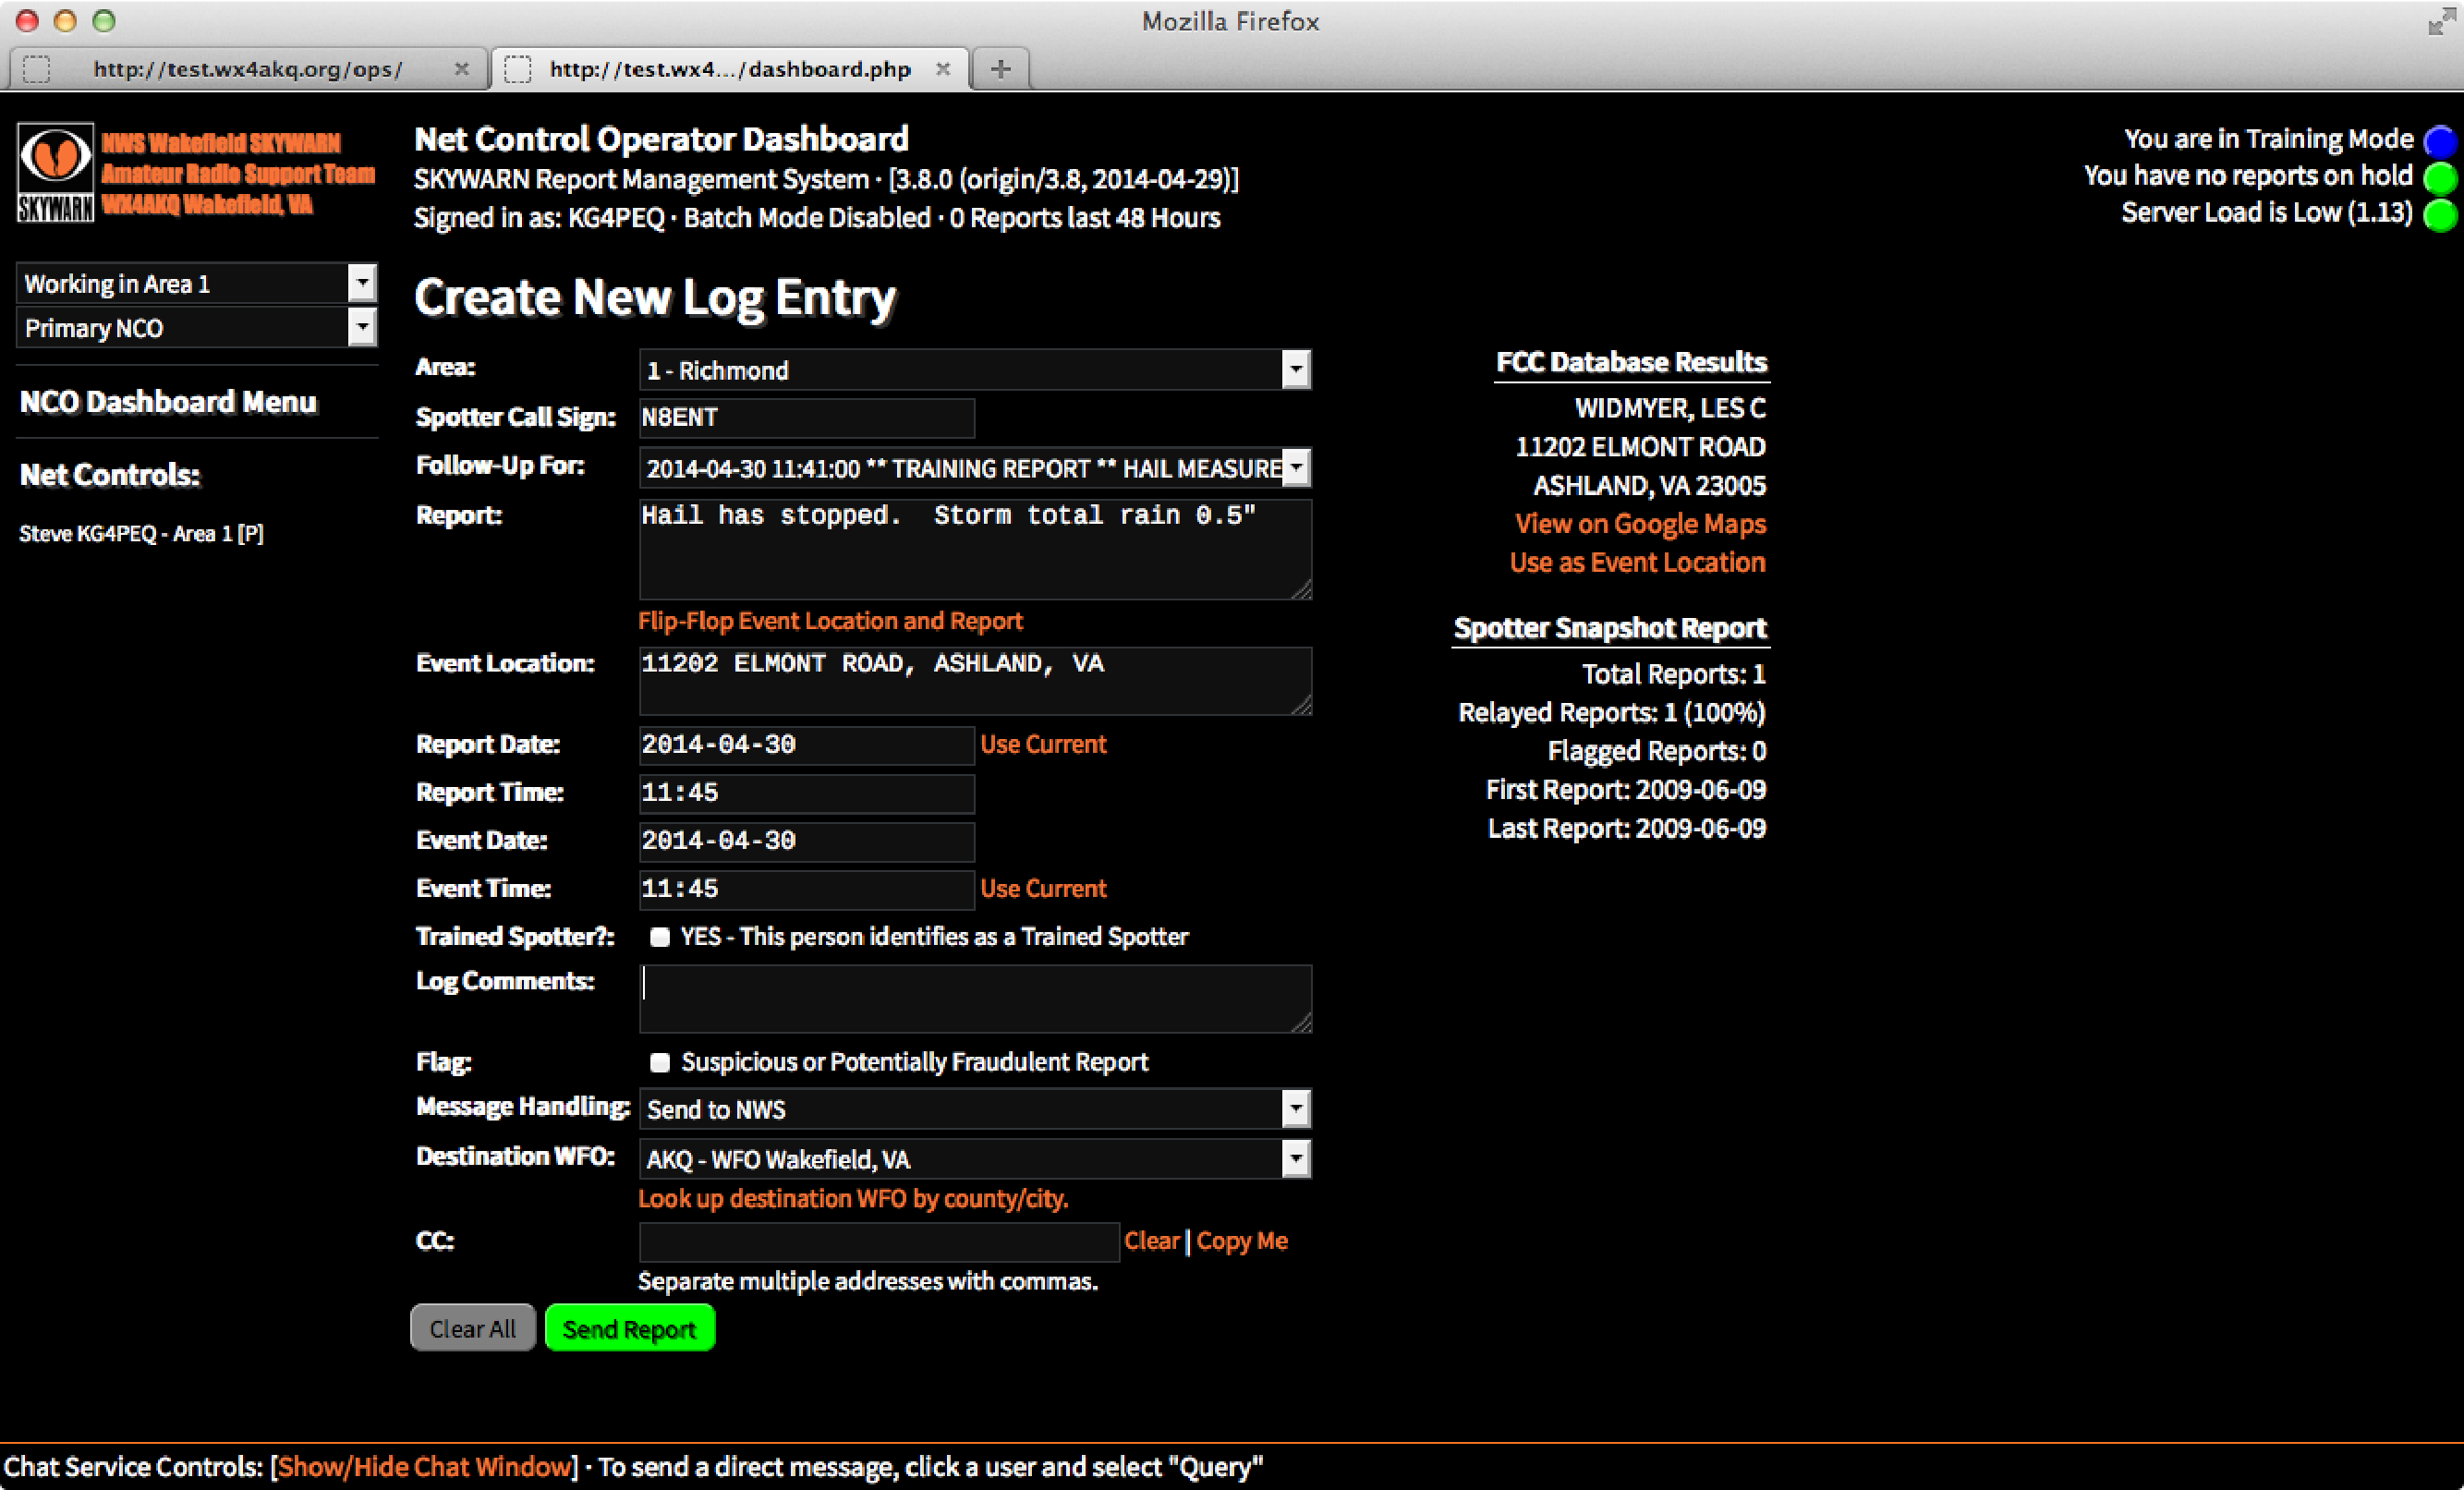
\includegraphics[width=\textwidth,keepaspectratio=true]{img/dash-followup-create}
  \caption{The \emph{Follow-Up For} dropdown populated with a list of previous reports.\label{fig:dash-followup-create}}
\end{figure}

When you click the a previous report, a little bit of magic happens.  The NCO Dashboard auto-populates the \emph{Location} field using the data from the last report.  The assumption is any follow-up will be for the same location.  If this is \emph{not} the case, a new report is usually needed, and \textbf{None - This is a new report} should be selected.

Once the report is submitted, one more piece of magic happens.  The reports are linked together in the log database.  This linking allows you to easily locate the original report and any follow-ups when viewing a report.  RMS is even smart enough to send both the new follow-up \emph{and} a copy of the original report to NWS when the report is released!

There is no limit to the number of follow-ups you can create for any given report.  You can also create a follow-up to a follow-up (to a follow-up to a follow-up...)

Anytime a Spotter calls in with a follow-up report, please utilize the follow-up functionality in the NCO Dashboard.  Since RMS will send both the old and new reports to NWS, this functionality helps NWS employees see the progression of events between the two individual reports.

\subsection{FCC Database Lookups}

When tabbing or clicking out of the \emph{Spotter Call Sign} field, the Log Entry from will automatically query the FCC database for the call sign and will display the licensee's name and address to the right of the form.

This information is presented to aid Net Control in identifying the station and verifying the correct call sign has been entered (look for incorrect names of known stations or out-of-state addresses).  Additionally, there are links to quickly view the Spotter's home address on Google Maps and use the listed address in the \emph{Event Location} information.

\orangebox{Careful!}{Use care in using the \emph{Use as Event Location} function.  Verify the Spotter's location is correct.  You might ask, ``are you at home on Elmont Road?''  Do not assume the address is correct.}

Licenses which are registered with anything other than a standard United States street address (for example, Post Office boxes) will display only partial information, such as the city and state.

A back-end process pulls down the full FCC database every Sunday and incremental updates once each day.

\subsection{Spotter Snapshot Report}

The Log Entry form will display a brief history of the Spotter's previous reports, specifically:

\begin{itemize}
\item Total number of reports.
\item Relayed Reports --- the number and percentage of reports which were determined to meet reporting criteria and were thus relayed to NWS.
\item Flagged Reports --- the number and percentage of reports which were flagged as suspicious or potentially fraudulent.
\item First and Last Reports
\end{itemize}

This data is presented to help you determine the level of scrutiny to give marginal or suspicious reports.

\orangebox{Careful!}{Use care not to make huge assumptions about the quality of a report based entirely on the Spotter Snapshot Report.  The skills and motives of Spotters can change over time.  A Spotter with a history of bad reports can eventually call in a good one, and vice-versa.  The information in the Spotter Snapshot Report is intended for use as a decision making aid, but should not be the only information considered when handling a Spotter report.}

%%%%%%%%%%%%%%%%%%%%%%%%%%%%%%%%%%%%%%%%%%%%%%%%%%%%%%%%%%%%%%%%%%%%%%%%

\section{Search Net Logs}\label{dash-search-logs}

The NCO Dashboard's Search function allows you to find past reports by any combination of Spotter call sign and date range.

If you want to search for reports which occurred only on one day, you would enter the same date for both the start and end date.

%%%%%%%%%%%%%%%%%%%%%%%%%%%%%%%%%%%%%%%%%%%%%%%%%%%%%%%%%%%%%%%%%%%%%%%%

\section{Area Roster}\label{dash-area-roster}

The \textbf{Area Roster} function of the NCO Dashboard presents an excerpt of the \nameref{team-roster}, showing only those team members assigned to your current SKYWARN Operating Area, as selected by the dropdown at the top left corner of the NCO Dashboard.

Note that this does \underline{not} account for team members who belong to one area but are currently signed into NCO Dashboard under another area.  For example, if a Net Control from Area 3 is running a net in Area 1, and is signed in under Area 1 in the NCO Dashboard, his Roster information still will not appear in the NCO Dashboard Area Roster function.

To view team members in other areas, use the \textbf{View All Areas} link at the bottom of the list.

%%%%%%%%%%%%%%%%%%%%%%%%%%%%%%%%%%%%%%%%%%%%%%%%%%%%%%%%%%%%%%%%%%%%%%%%

\section{Radio Reference}\label{dash-radio-ref}

The \textbf{Radio Reference} function displays the SKYWARN frequency information from our public-facing web site, based on your currently selected SKYWARN Operating Area.

In addition to the public information, any special information and instructions for Net Control Operators will be displayed.

Some of the information which might be displayed include:

\begin{itemize}
\item Repeater control codes
\item Control Operator names and phone numbers
\item Linking instructions
\item Routes in and out of the area via IRLP, Echolink, etc.
\end{itemize}

Only the information for your currently selected area will be displayed.  See \nameref{dash-set-area} on page \pageref{dash-set-area} for information on changing your selected area.

\orangebox{Protect Sensitive Information}{SKYWARN team members are obligated to maintain the confidentiality of the information presented in the \textbf{Radio Reference} area.  Repeater control codes, contact information, and other details displayed are for official SKYWARN use only.  Any unauthorized use or dissemination outside of SKYWARN is prohibited and may result in dismissal from the team.}

%%%%%%%%%%%%%%%%%%%%%%%%%%%%%%%%%%%%%%%%%%%%%%%%%%%%%%%%%%%%%%%%%%%%%%%%

\section{NWS Contact Information}\label{dash-send-email}

The \textbf{NWS Contact Information} section contains a list of NWS phone numbers, call signs, and e-mail addresses.  Clicking on the e-mail address will open a web form where you can quickly send a message to that office.

This is particularly handy if you have your own report to send to NWS.  Since you cannot log your own report in the NCO Dashboard, this e-mail tool provides a quick way to send the message.

You can e-mail any office which is supported by RMS.  See \nameref{rms-offices} on page \pageref{rms-offices} for a list of supported offices.

You will receive a copy of all e-mails sent through this tool for your own recordkeeping purposes.

E-mail messages sent through this function do not become a part of the permanent net logs.

%%%%%%%%%%%%%%%%%%%%%%%%%%%%%%%%%%%%%%%%%%%%%%%%%%%%%%%%%%%%%%%%%%%%%%%%

\section{Modify Global RMS Settings}\label{dash-rms-settings}

SKYWARN Leadership Team members can alter the behavior of RMS somewhat via the \textbf{Modify Global RMS Settings} function.

\begin{itemize}
\item \textbf{NWS Reporting.}  Turns NWS report relaying on or off.  Turning off NWS reporting does not prevent the creation or routing of new reports.  It simply suspends the automatic release and prevents Net Control Operators from manually releasing reports.  This is usually enabled during periods of system maintenance.
\item \textbf{Auto-Release Delay Time.}  Sets the age at which a report will qualify to be automatically released.  The default is 3 minutes.
\item \textbf{Batch Mode.}  Turns \nameref{rms-batch-mode} on or off.
\item \textbf{Batch Mode Release Interval.}  Specifies the interval at which new report batche are generated when Batch Mode is enabled.  The default is 30 minutes.
\end{itemize}

Changes to these settings impact all system users.

%%%%%%%%%%%%%%%%%%%%%%%%%%%%%%%%%%%%%%%%%%%%%%%%%%%%%%%%%%%%%%%%%%%%%%%%
%%%%%%%%%%%%%%%%%%%%%%%%%%%%%%%%%%%%%%%%%%%%%%%%%%%%%%%%%%%%%%%%%%%%%%%%
%%%%%%%%%%%%%%%%%%%%%%%%%%%%%%%%%%%%%%%%%%%%%%%%%%%%%%%%%%%%%%%%%%%%%%%%
%%%%%%%%%%%%%%%%%%%%%%%%%%%%%%%%%%%%%%%%%%%%%%%%%%%%%%%%%%%%%%%%%%%%%%%%
%%%%%%%%%%%%%%%%%%%%%%%%%%%%%%%%%%%%%%%%%%%%%%%%%%%%%%%%%%%%%%%%%%%%%%%%
%%%%%%%%%%%%%%%%%%%%%%%%%%%%%%%%%%%%%%%%%%%%%%%%%%%%%%%%%%%%%%%%%%%%%%%%

\chapter{Situation Awareness Dashboard}\label{sit-dashboard}

\section{Introduction}

The Situation Awareness Dashboard is a public-access web portal providing consolidated access to a variety of popular National Weather Service text and graphical forecast products, weather models, and radar data.  It has its origins in the former \emph{SKYWARN Partner Outreach Services Portal} which was retired in 2012.

Subscribers may receive one of several different access classes depending on their affiliation.  These access classes determine whether the subscriber may take advantage of certain services, such as read-only access to the SKYWARN net logs, chat, and the EMWIN e-mail weather alert system.

Members of the Wakefield SKYWARN Amateur Radio Support Team who have Ops Portal logins automatically have access to the Situation Awareness Dashboard with no additional registration required.

The dashboard is located at \url{http://situation.wx4akq.org/}.

%%%%%%%%%%%%%%%%%%%%%%%%%%%%%%%%%%%%%%%%%%%%%%%%%%%%%%%%%%%%%%%%%%%%%%%%

\section{Unrestricted Services}

Unrestricted services available to both registered and unregistered users include current radar images and a limited selection of forecast products.  All products originate from the National Weather Service and are pulled directly from NWS web sites.

There is no SKYWARN team-generated content available to unregistered users.

Additional information available includes general emergency information and utility outage information links.

Unrestricted services may be moved to and from restricted status as needed based on active emergency situations and subscription goals.

%%%%%%%%%%%%%%%%%%%%%%%%%%%%%%%%%%%%%%%%%%%%%%%%%%%%%%%%%%%%%%%%%%%%%%%%

\section{Restricted Services}

The following restricted services are available by subscription only:

\begin{itemize}
\item {\bf Current WWA's.}  Provides a list of all active watches, warnings, and advisories for the Wakefield County Warning area.  Product text is viewable within the browser.
\item {\bf Net Logs.}  Read-only access to the SKYWARN net logs with visibility into report details.
\item {\bf Ops Chat.}  Web-based chat client to allow direct interaction with SKYWARN Net Control Operators and leadership.
\item {\bf EMWIN Services.}  E-mail subscription to weather notifications powered by the EMWIN system.
\item {\bf \nameref{risk-tables-intro}.}  View access to our internal SKYWARN Risk Tables product.
\end{itemize}

%%%%%%%%%%%%%%%%%%%%%%%%%%%%%%%%%%%%%%%%%%%%%%%%%%%%%%%%%%%%%%%%%%%%%%%%

\section{Acceptable Use}

The Situation Awareness Dashboard is governed by the standard Wakefield SKYWARN Acceptable Use Policy (AUP) and the various IT systems policies included in the \href{http://www.wx4akq.org/manual.php}{SKYWARN Operations Manual\footnote{http://www.wx4akq.org/manual.php}}.  Users are asked to review and agree to these policies prior to registration and upon each login to the system.

\label{sec:eligibility}
\section{Subscriber Eligibility}

There are ten different access classes recognized by the Situation Awareness Dashboard:

\begin{itemize}
\item {\bf Unregistered user.} This is the default access class, available to anyone.  This is the most restricted access class.
\item {\bf Wakefield SKYWARN Net Control.}  This access class is given to anyone signing in to the Situation Awareness Dashboard with a \verb|@wx4akq.org| e-mail address.  Services available through Ops Portal must be managed through Ops Portal directly.  Users in this class will be directed back to Ops Portal for certain features.
\item {\bf Wakefield SKYWARN Spotter.}  Available to registered, active SKYWARN Spotters in the Wakefield CWA.
\item {\bf Neighboring SKYWARN Official/Net Control.}  Available to verified SKYWARN Net Control Operators (or similar position), including leadership officials, in immediately adjacent CWA's (LWX, MHX, PHI, RAH, or RNK).
\item {\bf NWS Employee.}  Available to NWS employees in the Wakefield WFO who are engaged in forecast operations.  Includes MIC, WCM, HMT, forecasters, and interns.  Must register with \verb|@noaa.gov| e-mail.
\item {\bf ARES Official or Appointed Position.}  Available to AEC, EC, ADEC, DEC and OES.
\item {\bf Local Emergency Management.}  Available to verified local (town/county/city) Emergency Management officials (EM, fire/police chief/sheriff, and similar roles) and agencies within the 66 counties and independent cities served by the Wakefield WFO.
\item {\bf State Emergency Management.}  Available to verified state Emergency Management officials and agencies in Virginia, Maryland, and North Carolina.
\item {\bf General Public/Other.}  Available to anyone.
\item {\bf General Public/Other --- Unrestricted.}  \emph{Future access class; not yet implemented.}
\end{itemize}

%%%%%%%%%%%%%%%%%%%%%%%%%%%%%%%%%%%%%%%%%%%%%%%%%%%%%%%%%%%%%%%%%%%%%%%%

\section{Registration Process}

The registration process can be completed online and, aside from account verification and approval, is entirely automated.  The process work flow is as follows:

\begin{enumerate}
\item User submits a registration request through the Situation Awareness Dashboard, via a registration link on the site.  The user will provide their contact details and self-identify for a specific access class.
\item A system-generated e-mail is sent to the user to verify their e-mail address.  The registration data is placed ``on hold'' until the address is verified.
\item Once the user clicks on the link provided in the verification e-mail, their registration details are sent to the \verb|leadership@wx4akq.org| e-mail list for action by any member of the Leadership Team.  Meanwhile, the user is provided with a randomly-generated password.
\item The Leadership Team takes action on the request.  Verification must be performed for most access classes.  This verification is described later in this manual.  The enrollment request may be approved or rejected.
\begin{itemize}
  \item If approving the request, the approver may override the user's requested access class with one more appropriate based on the outcome of the verification process.
  \item If appropriate, the request may be outright rejected.  A reason must be specified and will be shared with the requestor.  They may re-apply for a new account at any time.
  \end{itemize}
\item An e-mail is sent to the \verb|leadership@wx4akq.org| e-mail list with an approval or rejection notice for the applicant's request.
\end{enumerate}

%%%%%%%%%%%%%%%%%%%%%%%%%%%%%%%%%%%%%%%%%%%%%%%%%%%%%%%%%%%%%%%%%%%%%%%%

\section{Account Maintenance and Passwords}

Subscriber accounts can be viewed by Leadership Team members from within the Ops Portal web site, under ``Account Management.''  A broadcast e-mail link is provided for one-off instances in which a large number of subscribers must be contacted at once.

Password changes are self-guided from within the Situation Awareness Dashboard.  Password reset functionality for the Situation Awareness Dashboard is integrated into the Passport Password Management tool.  There is currently no capability for SKYWARN Leadership to forcibly reset a password.

At this time, there is no capability to modify or delete an account through the Ops Portal web site.  Certain changes, including account deletion, e-mail address updates, and access class modifications, can be accomplished via direct manipulation of the \verb|sitUsers| and \verb|alertSubs| MySQL tables on the server, and a web interface for these changes will be developed in the future.

%%%%%%%%%%%%%%%%%%%%%%%%%%%%%%%%%%%%%%%%%%%%%%%%%%%%%%%%%%%%%%%%%%%%%%%%

\section{Leadership Team Functions}\label{sit-leadership-functions}

\subsection{Verification Process}

SKYWARN Leadership Team members should neither blindly approve nor arbitrarily reject registration requests.  Whenever possible, an appropriate access class should be assigned at the time of approval.  It is the responsibility of the approver to ensure the user has been verified properly.

This section lists the verification process for each access class.

\subsubsection{Spotters}

Spotter accounts do not require special verification if a Spotter ID is provided in the registration request.  Since NWS no longer issues Spotter ID's, the Spotter may be asked to verify their last training date if desired, but in general, these registration requests are accepted with little to no verification required.

\subsubsection{Neighboring SKYWARN Official/Net Control}

Area Managers may already know the leadership contacts of neighboring SKYWARN teams and can utilize those connections for verification purposes.  If unable to verify affiliation, escalate to the Amateur Radio Coordinator.

\subsubsection{NWS Employee}

NWS employees of the Wakefield WFO must register under their \verb|@noaa.gov| e-mail address.  Verify they are listed on \href{http://www.erh.noaa.gov/er/akq/staff.php}{this web page\footnote{http://www.erh.noaa.gov/er/akq/staff.php}}.  If you cannot locate the employee on that web page, escalate the request to the Amateur Radio Coordinator for additional verification.

\subsubsection{ARES Official/Appointed Position}

Area Managers should already be familiar with the ARES EC's, AEC's, DEC's, and ADEC's within their assigned SKYWARN Operating Area.  If not, the state and district ARES web sites usually have an up-to-date directory.  These contacts can be used to verify OES and other ARES appointed positions.  If in doubt, escalate to the Amateur Radio Coordinator for verification.

\subsubsection{Local Emergency Management}

Local emergency management personnel, including Emergency Managers, police/fire chiefs, sheriffs, and the like, can be easily verified by checking the appropriate local government web site.  These registrations will also originate from a local government e-mail domain.

\subsubsection{State Emergency Management}

Similar eligibility and verification as Local Emergency Management accounts.

\subsubsection{General Public/Other}

No verification is required.

\subsection{Rejecting Registrations}

Account registration requests should \underline{rarely} be rejected.  Most registration requests can be approved as-is, and a few will require adjustment to the requested access class.

A few possible scenarios in which a request could be initially considered for rejection, and proposed solutions:

\begin{itemize}
\item {\bf Duplicate account.}  A user should have only one account.  If similarities in name or e-mail address raise suspicion of multiple accounts, the user should be contacted to determine the need for multiple accounts before taking action on the new request.  They may just need a password reset or e-mail address change on their original account.
\item {\bf Amateur radio team member.}  Members of the NWS Wakefield SKYWARN Amateur Radio Support Team should utilize their existing Ops Portal login for access to the Situation Awareness Dashboard.  No additional accounts should be created.
\end{itemize}

When rejecting a registration request, a reason must be provided.  This reason will be included in the e-mail notification of rejection sent to both the applicant and the \verb|leadership@wx4akq.org| e-mail list.  The notification will also indicate who rejected the request and will provide contact information.

\subsection{Changing E-mail Address}

At this time there is no web interface for changing the e-mail address associated with a Situation Awareness Dashboard user.  This change requires direct manipulation of two MySQL tables on the server.  Example commands are provided below.  For more information on accessing MySQL, including details on some graphical user interface (GUI) options to make this process much easier, see the \nameref{database-server} section starting on page \pageref{database-server}.

Connect to the MySQL server:

\begin{minted}[linenos=true]{text}
mysql --host=fujita.wx4akq.org --user=wx4akq --password
\end{minted}

Select the correct database and query for existing accounts matching the new e-mail address:

\begin{minted}[linenos=true]{mysql}
USE wx4akq;
SELECT * FROM sitUsers WHERE email='newaddress@host.com';
\end{minted}

If that query returns 0 rows, update both the \verb|sitUsers| and \verb|alertSubs| tables with the new e-mail address:

\begin{minted}[linenos=true]{mysql}
UPDATE sitUsers SET email='newaddress@host.com'
  WHERE email='oldaddress@host.com';
UPDATE alertSubs SET emailAddr='newaddress@host.com'
  WHERE emailAddr='oldaddress@host.com';
\end{minted}   

{\bf Note:}  The direct manipulation of the \verb|alertSubs| table may return a result of 0 rows changed.  This indicates the user is not currently subscribed to any EMWIN e-mail alerts.

Once this is done, manually edit the \verb|~/html/auth/.htpasswd_sit| file to change the user's e-mail address in the authentication database.

A more elegant, web based mechanism for accomplishing this type of change will be available in the future.

\begin{figure}[t]
  \centering
  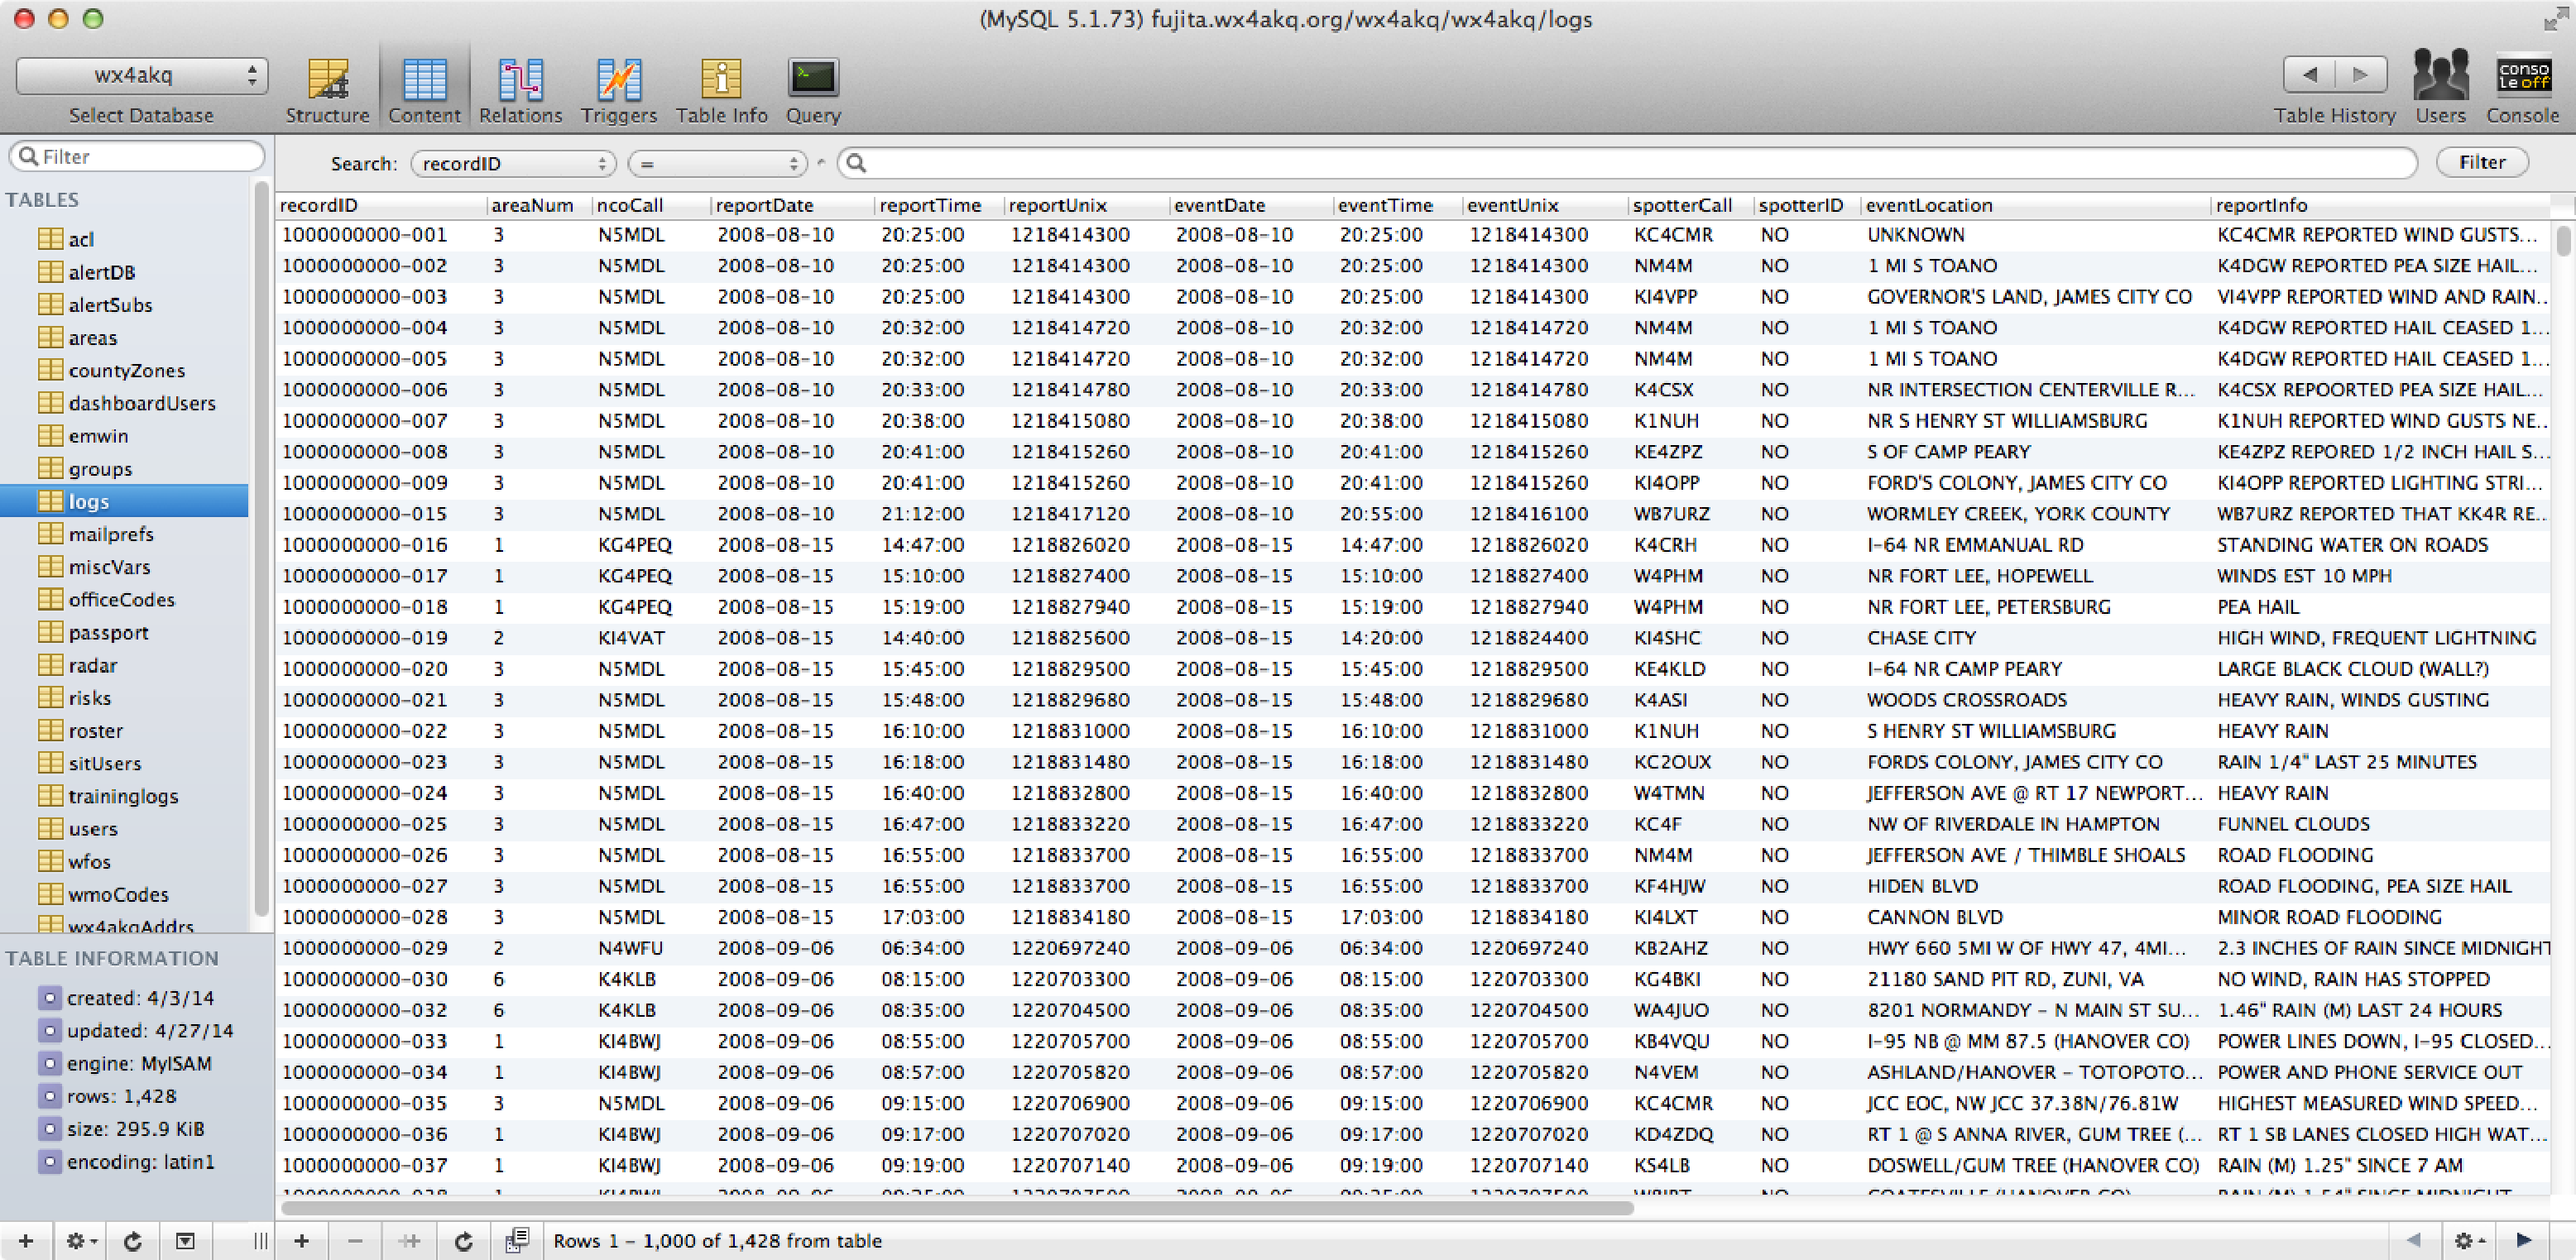
\includegraphics[width=\textwidth,keepaspectratio=true]{img/sequel-pro}
  \caption{In addition to conventional console access to MySQL, a number of graphical user interfaces (GUI's) are available for easier access and manipulation of MySQL databases and tables.  Shown here: \href{http://www.sequelpro.com/}{Sequel Pro} for Mac OS.  For more information MySQL GUI's, see \nameref{database-server} on page \pageref{database-server}.\label{fig:sequel-pro}}
\end{figure}

\subsection{Changing Access Class}

Changing the user's access class requires direct manipulation of the \verb|sitUsers| MySQL table on the server.

Connect to the MySQL server:

\begin{minted}[linenos=true]{text}
mysql --host=fujita.wx4akq.org --user=wx4akq --password
\end{minted}

Select the correct database and update the table with the new access class:

\begin{minted}[linenos=true]{mysql}
USE wx4akq;
UPDATE sitUsers SET acctType='newclass' WHERE email='user@domain.com';
\end{minted}

\verb|acctType| may be any of the following:  \verb|spotter|, \verb|neighbor|, \verb|nws|, \verb|ares|, \verb|lem|, \verb|sem|, \verb|public|, or \verb|public-unr| (not yet implemented).  More information can be found in \hyperref[sec:eligibility]{Subscriber Eligibility}.

\subsection{Account Conversion Tools}\label{sit-account-conversion}

Beginning with RMS version 3.8 in May 2014, tools to convert an account between an Ops Portal account and a Situation Awareness Dashboard account are included in the Account Management portion of Ops Portal.

When a Situation Awareness Dashboard user becomes a Net Control Operator, or when a Net Control Operator leaves the team and wishes to be converted to a Situation Awareness Dashboard user, the use of these conversion tools will:

\begin{itemize}
\item Preserve the user's EMWIN e-mail alert subscriptions;
\item Transfer user information (name, phone number, e-mail) between systems;
\item Maintain the user's password
\end{itemize}

The use of direct manipulation of the MySQL databases for purposes of account conversion (as described in previous versions of this reference manual) is discouraged.

%%%%%%%%%%%%%%%%%%%%%%%%%%%%%%%%%%%%%%%%%%%%%%%%%%%%%%%%%%%%%%%%%%%%%%%%
%%%%%%%%%%%%%%%%%%%%%%%%%%%%%%%%%%%%%%%%%%%%%%%%%%%%%%%%%%%%%%%%%%%%%%%%
%%%%%%%%%%%%%%%%%%%%%%%%%%%%%%%%%%%%%%%%%%%%%%%%%%%%%%%%%%%%%%%%%%%%%%%%
%%%%%%%%%%%%%%%%%%%%%%%%%%%%%%%%%%%%%%%%%%%%%%%%%%%%%%%%%%%%%%%%%%%%%%%%
%%%%%%%%%%%%%%%%%%%%%%%%%%%%%%%%%%%%%%%%%%%%%%%%%%%%%%%%%%%%%%%%%%%%%%%%
%%%%%%%%%%%%%%%%%%%%%%%%%%%%%%%%%%%%%%%%%%%%%%%%%%%%%%%%%%%%%%%%%%%%%%%%

\chapter{Team Network Share}\label{team-network-share}

All SKYWARN team members with a valid Ops Portal login have access to a network file share which operates based on the standard WebDAV protocol.  Portions of the Team Network Share are publicly available in the form of our online file library.

%%%%%%%%%%%%%%%%%%%%%%%%%%%%%%%%%%%%%%%%%%%%%%%%%%%%%%%%%%%%%%%%%%%%%%%%

\section{Accessing the Share}

The contents of the Team Network Share can be viewed through any web browser.  No special software is required for viewing and downloading files.

Computers, tablets, and smart phones can read and write from the network share either via built-in network access functions or downloaded third-party applications.

The Team Network Share is located at \texttt{http://files.wx4akq.org/webdav}.

\orangebox{Note}{The \texttt{http://files.wx4akq.org/webdav} URL is the address to supply to your WebDAV client software.  If you simply wish to browse the Team Network Share from your web browser, you should instead go to \href{http://go.wx4akq.org/share}{http://go.wx4akq.org/share}.\\\\Either way, you will log in with your Ops Portal user name and password.  You can use the Passport tool to perform a reset if you do not know your login credentials.}

%%%%%%%%%%%%%%%%%%%%%%%%%%%%%%%%%%%%%%%%%%%%%%%%%%%%%%%%%%%%%%%%%%%%%%%%

\section{Authentication}

The Team Network Share utilizes the standard Apache \texttt{.htpasswd} and \texttt{.htgroups} files located in the \texttt{/var/www/auth/} folder.  The content of these files is controlled by the normal Ops Portal user provisioning process.

%%%%%%%%%%%%%%%%%%%%%%%%%%%%%%%%%%%%%%%%%%%%%%%%%%%%%%%%%%%%%%%%%%%%%%%%

\section{Password Restrictions}

Standard Apache \texttt{.htaccess} files can be used to restrict access to files or folders on the share.

Here is a sample \texttt{.htaccess} file to restrict access based on the following rules:

\begin{itemize}
\item The user must be logged in to get to the folder (not publicly accessible)
\item The user must be a member of the \texttt{leadership} group to access the \texttt{pwlist*} files.
\item The user \texttt{sysop} is the only one who can access the \texttt{pwlist-server.txt} file.
\end{itemize}

\begin{minted}[linenos=true]{apacheconf}
AuthName "WX4AKQ Team Network Share"
AuthType Basic

Options +Indexes
require valid-user

<Files pwlist*>
	require group leadership
</Files>

<Files pwlist-server.txt>
	require user sysop
</Files>
\end{minted}

\orangebox{Warning}{File and folder access restrictions do not apply to direct shell or SFTP access.  This means anyone who has the ability to log in to the server as user \texttt{wx4akq} or a superuser will be able to view the files/folders.  Keep this in mind when storing particularly sensitive information.}

%%%%%%%%%%%%%%%%%%%%%%%%%%%%%%%%%%%%%%%%%%%%%%%%%%%%%%%%%%%%%%%%%%%%%%%%

\section{Cautionary Note on File Paths}

Many documents in publicly-accessible folders are directly linked (``hotlinked'') from the various SKYWARN web sites.  Use extreme care in renaming any public folders or files, or changing the location of any public folders or files, to ensure no documents become inaccessible.

%%%%%%%%%%%%%%%%%%%%%%%%%%%%%%%%%%%%%%%%%%%%%%%%%%%%%%%%%%%%%%%%%%%%%%%%

\section{Connecting to the Team File Share}

\subsection{Connecting from Windows}

These instructions are for Windows 7. The process in other Windows versions will be similar.

\begin{itemize}
\item Click on the Start Menu and then \texttt{My Computer}.
\item Click \texttt{Map Network Drive}.
\item Select a drive letter to use.
\item Enter \texttt{http://files.wx4akq.org/webdav} for the server address.
\item Check the \texttt{Log in with different credentials} box.
\item Connect and log in with your Ops Portal credentials.
\end{itemize}

If you encounter errors during this process you may need to download and run \href{http://files.wx4akq.org/Software/misc/Win7\_WebDAV\_Fix.zip}{this registry patch}\footnote{http://files.wx4akq.org/Software/misc/Win7\_WebDAV\_Fix.zip}. Download and decompress the \texttt{Win7\_WebDAV\_Fix.zip} file, double-click the included \texttt{.reg} file, and reboot before attempting to connect again. This registry fix is for Windows 7 only. Windows XP users may need \href{http://www.microsoft.com/en-us/download/details.aspx?id=15123}{this Windows software update}\footnote{http://www.microsoft.com/en-us/download/details.aspx?id=15123}.

There are additional registry fixes required to allow Microsoft Office to operate over a WebDAV link. Microsoft has \href{http://support.microsoft.com/kb/2123563}{this Knowledge Base article}\footnote{http://support.microsoft.com/kb/2123563} on the subject, and we have a \href{http://files.wx4akq.org/Software/misc/Office\_2010\_Fix.zip}{quick registry fix for Office 2010}\footnote{http://files.wx4akq.org/Software/misc/Office\_2010\_Fix.zip}.

\subsection{Connecting from Mac OS X}

From Finder, press Command+K or select the \texttt{Go} menu and then \texttt{Connect to Server}.  For the server address, enter \texttt{http://files.wx4akq.org/webdav} and click \texttt{Connect}.  Select the option to connect as a registered user and use your Ops Portal credentials to connect.

\subsection{Connecting from iOS}

Recommended iPhone/iPad software is \href{https://itunes.apple.com/us/app/webdav-nav+/id412341302?mt=8}{WebDAV Nav+}\footnote{https://itunes.apple.com/us/app/webdav-nav+/id412341302?mt=8} (\$3.99). Configuration:

\begin{itemize}
\item \texttt{Name}: SKYWARN WebDAV
\item \texttt{Server URL}: http://files.wx4akq.org/webdav
\item \texttt{Username}: kg4peq
\item \texttt{Password}: (your Ops Portal password)
\item \texttt{Directory tree fallback}: Off
\end{itemize}

%%%%%%%%%%%%%%%%%%%%%%%%%%%%%%%%%%%%%%%%%%%%%%%%%%%%%%%%%%%%%%%%%%%%%%%%
%%%%%%%%%%%%%%%%%%%%%%%%%%%%%%%%%%%%%%%%%%%%%%%%%%%%%%%%%%%%%%%%%%%%%%%%
%%%%%%%%%%%%%%%%%%%%%%%%%%%%%%%%%%%%%%%%%%%%%%%%%%%%%%%%%%%%%%%%%%%%%%%%
%%%%%%%%%%%%%%%%%%%%%%%%%%%%%%%%%%%%%%%%%%%%%%%%%%%%%%%%%%%%%%%%%%%%%%%%
%%%%%%%%%%%%%%%%%%%%%%%%%%%%%%%%%%%%%%%%%%%%%%%%%%%%%%%%%%%%%%%%%%%%%%%%
%%%%%%%%%%%%%%%%%%%%%%%%%%%%%%%%%%%%%%%%%%%%%%%%%%%%%%%%%%%%%%%%%%%%%%%%

% \chapter{System Administration}

%%%%%%%%%%%%%%%%%%%%%%%%%%%%%%%%%%%%%%%%%%%%%%%%%%%%%%%%%%%%%%%%%%%%%%%%




%%%%%%%%%%%%%%%%%%%%%%%%%%%%%%%%%%%%%%%%%%%%%%%%%%%%%%%%%%%%%%%%%%%%%%%%
%%%%%%%%%%%%%%%%%%%%%%%%%%%%%%%%%%%%%%%%%%%%%%%%%%%%%%%%%%%%%%%%%%%%%%%%
%%%%%%%%%%%%%%%%%%%%%%%%%%%%%%%%%%%%%%%%%%%%%%%%%%%%%%%%%%%%%%%%%%%%%%%%
%%%%%%%%%%%%%%%%%%%%%%%%%%%%%%%%%%%%%%%%%%%%%%%%%%%%%%%%%%%%%%%%%%%%%%%%
%%%%%%%%%%%%%%%%%%%%%%%%%%%%%%%%%%%%%%%%%%%%%%%%%%%%%%%%%%%%%%%%%%%%%%%%
%%%%%%%%%%%%%%%%%%%%%%%%%%%%%%%%%%%%%%%%%%%%%%%%%%%%%%%%%%%%%%%%%%%%%%%%

\chapter{Content Management}

%%%%%%%%%%%%%%%%%%%%%%%%%%%%%%%%%%%%%%%%%%%%%%%%%%%%%%%%%%%%%%%%%%%%%%%%

The 6 major WX4AKQ.org web sites and 1 supporting collection of resource files are maintained on the main SKYWARN cluster, accessible via SSH by logging in as \texttt{wx4akq@fujita.wx4akq.org}.

The files are managed by the Git Source Code Management tool.  

For more information or to learn how to use Git, see \href{http://www.gitscm.com/}{GitSCM.com}.

%%%%%%%%%%%%%%%%%%%%%%%%%%%%%%%%%%%%%%%%%%%%%%%%%%%%%%%%%%%%%%%%%%%%%%%%

\section{Accessing the Server}

The primary SKYWARN server is called \texttt{fujita} and it can be accessed directly using Secure Shell (SSH).  Use any SSH software to connect to \texttt{wx4akq@fujita.wx4akq.org}.  SSH provides console-level access to the server and, with elevated permissions, access to core server software and settings.  Web site content can also be modified via SSH.  However, some content can be submitted in Markdown format via the team network share, or online editing tools provided within Ops Portal.  Using the team network share or online editing tools do not require the use of SSH.

For security reasons, all non-essential ports are sealed off by an \texttt{iptables} firewall.  Additionally, direct login to the \texttt{root} account is disabled.  Once logged in as a regular user, it is possible to \texttt{su} and provide the \texttt{root} password to gain administrative privileges.

%%%%%%%%%%%%%%%%%%%%%%%%%%%%%%%%%%%%%%%%%%%%%%%%%%%%%%%%%%%%%%%%%%%%%%%%

\section{Git Repo Folders}

Each web site is managed through a Git repository located in the \texttt{\~\//git/} folder.

\begin{verbatim}
 ~/git/www-emwin      # EMWIN web site
 ~/git/www-ops        # Ops Portal  
 ~/git/www-passport   # Passport password tool
 ~/git/www-pub        # Public wx4akq.org site
 ~/git/www-resources  # Resource folders
 ~/git/www-sit        # Situation` Awareness Dashboard
 ~/git/www-training   # Training portal
\end{verbatim}

\orangebox{Warning}{As with any Git repository, it is extremely important that the files and folders under \texttt{\~\//git/} are \emph{never} modified directly.}

%%%%%%%%%%%%%%%%%%%%%%%%%%%%%%%%%%%%%%%%%%%%%%%%%%%%%%%%%%%%%%%%%%%%%%%%

\section{Web Server Folders}

The folders on the production web server are maintained via a Git clone.  These files should never be edited directly, with the exception of the \texttt{.htaccess} file in each \texttt{sites/} folder, as well as the \texttt{globals.php} file in \texttt{resources}, both of which are not included in the Git repos (excluded via \texttt{.gitignore}).

These folders represent the current \texttt{master} branch of each repo.  Most of our web sites require the global \texttt{resources/} folder, which is just a symlink to\\\texttt{/var/www/sites/resources/}.

\begin{verbatim}
/var/www/auth/             # Authentication resources *
/var/www/sites/emwin/      # EMWIN site
/var/www/sites/files/      # File library and WebDAV *
/var/www/sites/ops/        # Ops Portal
/var/www/sites/passport/   # Passport password tool
/var/www/sites/pub/        # Main wx4akq.org site
/var/www/sites/resources/  # Resource folders
/var/www/sites/sit/        # Situation Dashboard
/var/www/sites/training/   # Training Portal
/var/www/sites/utils/      # Utilities folder *
/var/www/sites/test/       # Test Area (see below)
/var/www/sites/itweb/      # IT Support Web Site

 * = not maintained via Git
\end{verbatim}

%%%%%%%%%%%%%%%%%%%%%%%%%%%%%%%%%%%%%%%%%%%%%%%%%%%%%%%%%%%%%%%%%%%%%%%%

\section{Test Server}

The test area located under \texttt{/var/www/sites/test/} is designed to provide a live development workspace on the web server for design and testing of updates to the SKYWARN web sites.

Each folder in the test area is another clone of the Git repo for each site, with the exception of the \texttt{auth/} folder, which is a symbolic link back to the main\\\texttt{/var/www/sites/auth/} folder.

This structure permits the use of a common authentication database and credential set across both the test server and the production server.

All edits to any Git-managed SKYWARN web site must be performed in a new Git branch on the test server first, and, once verified for accuracy and performance, can be merged to the \texttt{master} branch and rolled to the production server.

%%%%%%%%%%%%%%%%%%%%%%%%%%%%%%%%%%%%%%%%%%%%%%%%%%%%%%%%%%%%%%%%%%%%%%%%

\section{The Update Workflow}

These steps assume you are working over a remote login to fujita using SSH, and are working with files in the test area.  For this example, we will look at making updates to the public-facing \texttt{www.wx4akq.org} web site.

\subsection{Create a Test Workspace (Optional)}

If there is not already a test workspace for the web site to be modified, create one and link to the test \texttt{resources/} folder:

\begin{minted}[linenos=true]{text}
mkdir /var/www/sites/test/pub/
cd /var/www/sites/test/pub/
git clone ssh://wx4akq@fujita.wx4akq.org/home/wx4akq/git/www-pub .
ln -s /var/www/sites/test/resources/ ./resources/
\end{minted}

\subsection{Create a new Remote Branch}

Changes should never be committed directly to the `master` branch!  Always create a new remote branch for the set of changes you are about to make and be sure to push that branch to the server.

First, check out the master branch and pull from the server:

\begin{minted}[linenos=true]{text}
git checkout master
git pull
\end{minted}

Then create your new remote branch and push it to the server.  Your remote branch should have a meaningful name.

If you are making only minor content edits, use \texttt{changes-} followed by the date in ``yyyymmdd'' format.  For example, \texttt{changes-20140511}:

\begin{minted}[linenos=true]{text}
git checkout -b changes-20140511
git push -u origin changes-20140511
\end{minted}

\subsection{Make the Changes and Commit to Git}

Make your changes, which can be viewed at \texttt{http://test.wx4akq.org/sitename/}:

\begin{minted}[linenos=true]{text}
nano -w index.php
nano -w area1.php
# [..etc..]
\end{minted}

Add any new or changed files to the commit:

\begin{minted}[linenos=true]{text}
git add index.php
git add newfile.php
# [..etc..]
\end{minted}

Or, alternatively, \texttt{git commit -a} to commit all changed files.

Perform a check for any uncomitted files:

\begin{minted}[linenos=true]{text}
git status
\end{minted}

Commit the changes and add a comment:

\begin{minted}[linenos=true]{text}
git commit -m 'Added upcoming class information'
\end{minted}

Finally, push the commit to the repo:

\begin{minted}[linenos=true]{text}
git push
\end{minted}

\subsection{Plan A: Merge to Master and Go Live}\label{publish-plan-a}

In almost all cases, the work performed on branches on the test server will need to be merged into \texttt{master} and pushed to the production server.  These steps will be performed in the test server folders:

Do a final check for any uncommitted changes:

\begin{minted}[linenos=true]{text}
git status
\end{minted}

Run \texttt{git commit} if there are uncommitted changes.

Do a final push to the repo:

\begin{minted}[linenos=true]{text}
git push
\end{minted}

Check out the \texttt{master} branch, then merge in the \texttt{changes-} branch and push the new \texttt{master} up to the repo:

\begin{minted}[linenos=true]{text}
git checkout master
git merge changes-20140511
git push
\end{minted}

Now pull the new \texttt{master} to the production server:

\begin{minted}[linenos=true]{text}
cd /var/www/sites/pub/
git checkout master
git pull
\end{minted}

The production server is now up-to-date with the changes introduced in the \texttt{changes-} branch.

\subsection{Plan B: Go Live with the Branch}

In some cases, it may be preferable \emph{not} to merge the new branch into \texttt{master} and instead directly deploy the branch on the production server.

This approach can be beneficial in the case of a large version update to a critical system which may have undetected bugs, necessitating a quick rollback to the previous version.  Once the code is found to be stable, it can then be merged into \texttt{master}.

Starting in the test server folder, do a final check for any uncommitted changes:

\begin{minted}[linenos=true]{text}
git status
\end{minted}

Run \texttt{git commit} if there are uncommitted changes.

Do a final push to the repo:

\begin{minted}[linenos=true]{text}
git push
\end{minted}

Switch to the production server folder and pull from the repo:

\begin{minted}[linenos=true]{text}
cd /var/www/sites/pub/
git pull
\end{minted}

List the remote branches to ensure the desired branch appears:

\begin{minted}[linenos=true]{text}
git branch -r
\end{minted}

Check out the branch:

\begin{minted}[linenos=true]{text}
git checkout changes-20140511
\end{minted}

If a rollback to the previous version is necessary, this can be performed by simply checking out the current \texttt{master}:

\begin{minted}[linenos=true]{text}
git checkout master
\end{minted}

Once the code is determined to be stable and a merge to \texttt{master} is desired, see the steps for \nameref{publish-plan-a} on page \pageref{publish-plan-a} to merge the branch to \texttt{master}, push it to the git repo, and roll it out to the production server.

\subsection{Branch Deletion Policy}

As a matter of policy, all branches should remain in the git repository.  Do not remove any branch, even once it has been merged into \texttt{master}. In the event a branch was erroneously created and needs to be removed, the following commands will remove it:

\begin{minted}[linenos=true]{text}
git push origin :branchname
git push origin :refs/origin/branchname
\end{minted}

\subsection{Resolving Merge Conflicts}

See \href{http://bit.ly/1me7wTh}{this page}\footnote{http://bit.ly/1me7wTh} for assistance resolving conflicts with merges.

\subsection{Cloning a Project Locally}

With the \texttt{~/.ssh/id\_wx4akq} key (from \texttt{fujita}) added to your local SSH installation using \texttt{ssh-add id\_wx4akq} you can create a local clone of the repository:

\begin{minted}[linenos=true]{text}
# Create the project folder and do the clone
mkdir ~/projects
git clone ssh://wx4akq@fujita.wx4akq.org/home/wx4akq/git/www-pub ~/projects/pub

# Get and link the resources folder
git clone ssh://wx4akq@fujita.wx4akq.org/home/wx4akq/git/www-resources ~/projects/resources
ln -s ~/projects/pub/resources ~/projects/resources
\end{minted}

\subsection{Creating a New Site \& Repo from Scratch}

To create a new web site project from scratch:

Create the repo folder and initialize it:

\begin{minted}[linenos=true]{text}
mkdir ~/git/newsite
cd ~/git/newsite
git --bare init
\end{minted}

Clone the empty repo to the test server:

\begin{minted}[linenos=true]{text}
git clone ssh://wx4akq@fujita.wx4akq.org/home/wx4akq/git/newsite /var/www/sites/test/newsite/
\end{minted}

(A warning about cloning an empty repository is normal.)

Link to resources if needed:

\begin{minted}[linenos=true]{text}
ln -s /var/www/sites/test/resources /var/www/sites/test/newsite/resources
\end{minted}

The site is browsable at \texttt{http://test.wx4akq.org/newsite/}.

%%%%%%%%%%%%%%%%%%%%%%%%%%%%%%%%%%%%%%%%%%%%%%%%%%%%%%%%%%%%%%%%%%%%%%%%

\section{Page Template}

The following page template should be used for all pages to incorporate our standard style on public and internal sites.
\pagebreak
\begin{minted}[linenos=true]{php}
<?php include("resources/includes.php");?>
<HEAD>
 <LINK REL="stylesheet" TYPE="text/css" HREF="resources/styles.css" />
 <TITLE><!-- page title here --></TITLE>
</HEAD>
<BODY><?php buildpagetop();?>
<!-- DOCUMENT BODY HERE -->

<!-- END DOCUMENT BODY --->
<?php buildpagefooter();?></TD></TR></TABLE>
</BODY>
</HTML>
\end{minted}

%%%%%%%%%%%%%%%%%%%%%%%%%%%%%%%%%%%%%%%%%%%%%%%%%%%%%%%%%%%%%%%%%%%%%%%%

\section{PHP Markdown Support}

The \texttt{resources} library includes \href{http://michelf.ca/projects/php-markdown/}{Michel Fortin's PHP Markdown}\footnote{http://michelf.ca/projects/php-markdown/} to include Markdown code in the SKYWARN web sites.

With \texttt{resources/includes.php} included in a PHP file, the Michelf PHP Markdown library is automatically initialized.  If you are not including our \texttt{includes.php} file, the following code is necessary to initialize the Markdown functions:

\begin{minted}[linenos=true]{php}
<?php
# Install PSR-0-compatible class autoloader
spl_autoload_register(function($class){
	require preg_replace('{\\\\|_(?!.*\\\\)}', \
	DIRECTORY_SEPARATOR, ltrim($class, '\\')).'.php';
});
# Get Markdown class
use Michelf\Markdown;
?>
\end{minted}

With our \texttt{includes.php} included in a PHP file, a number of custom Markdown-related functions are available.  See the \texttt{includes.php} file for more information.

%%%%%%%%%%%%%%%%%%%%%%%%%%%%%%%%%%%%%%%%%%%%%%%%%%%%%%%%%%%%%%%%%%%%%%%%

\section{Markdown Bulletins on Ops Portal and the Public Front Pages}\label{markdown-bulletins}

Code included in the front pages of Ops Portal and the public web site makes it very easy for anyone with minimal technical knowledge to post short bulletins to our web pages using the simple Markdown format.

This section discusses where to place those files.

\subsection{Markdown Style Guide}

Basic \href{http://daringfireball.net/projects/markdown/syntax}{Markdown syntax}\footnote{http://daringfireball.net/projects/markdown/syntax} is supported.  All headings should be at level 2 (\texttt{\#\#}) or deeper.  Headings generated at level 1 (\texttt{\#}) will not display correctly.

\subsection{Posting Markdown to the Server}

There are two methods for posting Markdown bulletins on Ops Portal and the public web site.  You may either use the built-in editing tools available via Ops Portal, or directly upload the files using the WebDAV network share.

The built-in editing tools, under ``Area Manager Tools'' on Ops Portal, provide a web-based interface for creating, viewing, and deleting bulletins on the Ops Portal and public web sites.

\orangebox{Quick Tip}{The built-in editing tools are the preferred method for working with bulletins on the Ops Portal and public web sites and require the least amount of technical knowledge.}

When using the WebDAV network share to place files on the server, the Markdown files go in one of the two subfolders under \texttt{/www\_markdown/ops} or \texttt{/www\_markdown/pub} folder, either \texttt{routine} for routine bulletins or \texttt{urgent} for high priority bulletins.  The full path for an urgent bulletin for Ops Portal would be \texttt{/www\_markdown/ops/urgent}.  File names do not matter, as long as the file ends with the \texttt{.md} extension (in lowercase).  The server will sort the files in reverse order by modification time, newest files first, when displaying them on the site.

\begin{figure}[t]
  \centering
  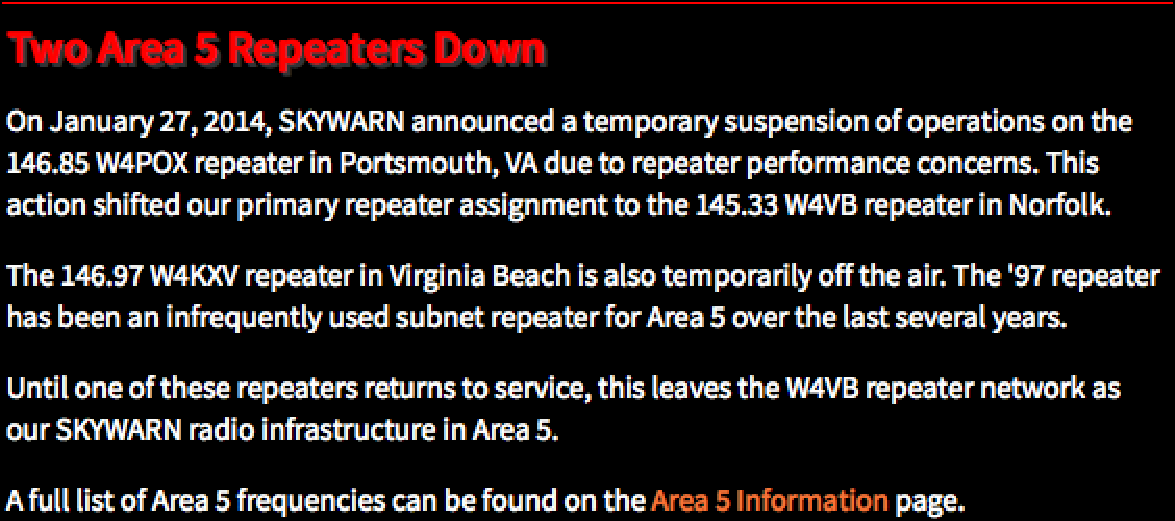
\includegraphics[width=\textwidth,keepaspectratio=true]{img/urgent-bulletin}
  \caption{Urgent bulletin displayed on the public web site.\label{fig:urgent-bulletin}}
\end{figure}

Bulletins on Ops Portal and the public web site may be classified as either ``routine'' or ``urgent.''  Urgent bulletins, such as the one shown in Figure \ref{fig:urgent-bulletin}, receive special formatting to make them stand out.  Urgent bulletins also appear before routine bulletins on both sites.

When creating bulletins, the classification -- urgent vs. routine -- is determined solely by which folder the bulletin is placed in.  The priority can be changed by moving the file from the \texttt{urgent/} folder to the \texttt{routine/} folder, or vice-versa.

%%%%%%%%%%%%%%%%%%%%%%%%%%%%%%%%%%%%%%%%%%%%%%%%%%%%%%%%%%%%%%%%%%%%%%%%

\section{Markdown Content on Area Pages}

The Area Information Pages on the public web site and within the \nameref{nco-dashboard} contain links to three specific Markdown files and one Markdown news bulletin folder, all of which are specific to each area.

These files must be submitted via WebDAV using the team network share.  There is no web interface for editing these files at this time.

Each area has its own folder on the network share.  For example, Area 1 files are stored under \texttt{/www\_markdown/area\_pages/area1}.

Three specialized files can be stored here and must named as follows:

\begin{itemize}
\item \texttt{area1-info.md}: This file stores long-term, fairly static information about the area, such as any special notes on repeater coverage, subnet boundaries, net sponsors, etc.  This file, if it exists, is inserted below the ``Repeater Information'' section.
\item \texttt{area1-pub.md}: This file contains any information which might be of interest to the general public but which may be redundant to our team members.  This file is displayed when the Area Information page is viewed from the public web site but is suppressed when viewed from within the NCO Dashboard.
\item \texttt{area1-private.md}:  This file contains special instructions and other information specifically for our Net Control Operators.  It is not displayed when the Area Information page is viewed from the public web site and is only available when accessed from within the NCO Dashboard.
\end{itemize}

The style guidelines are the same as the public site and Ops Portal bulletins:  all headings must be level 2 (\texttt{\#\#}) or lower;  level 1 (\texttt{\#}) headings will not display correctly.

Each area also has a \texttt{news/} folder which operates in a similar manner to the news folders used on the public site and Ops Portal, except there is no provision for ``urgent'' bulletins.  Individual Markdown files placed in an area's \texttt{news/} folder are displayed in reverse order by modification time, with newest files displayed first.  These files are only displayed when viewed from the public web site.  Display is suppressed when viewed from the NCO Dashboard.

%%%%%%%%%%%%%%%%%%%%%%%%%%%%%%%%%%%%%%%%%%%%%%%%%%%%%%%%%%%%%%%%%%%%%%%%

\section{Database Server}\label{database-server}

The database server used by the SKYWARN sites is also hosted on Fujita.  It is a \href{http://www.mysql.org}{MySQL}\footnote{http://www.mysql.org/} server listening on port 3306.  For security reasons, the user accounts on the MySQL server are bound to specific IP addresses, and it is generally not possible to directly access the MySQL server directly from outside the SKYWARN server (though port 3306 \emph{is} open in \texttt{iptables} for purposes of database replication).

Direct manipulation of the MySQL databases is possible from the Linux console via remote SSH login.  To directly manipulate the MySQL databases from outside the SKYWARN server, there are two options:

\begin{itemize}
\item Establish an SSH tunnel between your local machine and the MySQL server;  then run your local MySQL command-line client over the tunnel.

\item Use GUI software capable of establishing the SSH tunnel and MySQL link for you, such as \href{http://www.sequelpro.com/}{Sequel Pro}\footnote{http://www.sequelpro.com/} or \href{http://www.heidisql.com/}{HeidiSQL}\footnote{http://www.heidisql.com/}.
\end{itemize}

With either method, since an SSH tunnel is used, bound to the loopback interface on \texttt{fujita}, the MySQL server will see the connection as local and will permit login to any user account permitted to connect from the loopback interface.

\subsection{MySQL Basics}

MySQL is one of the most popular database servers in use today.  We use it to store lots of different kinds of data, like our roster, repeater listings, and net logs.  The other pieces of software that drive our web server read and write to the MySQL databases to create the dynamic elements of our web site.

In many cases user-friendly web forms and other utilities can provide all the access most of our team members will ever need.  Sometimes, though, it is necessary to perform a more complex data lookup or you might need to directly edit some of the information in our records.

The GUI's discussed here will allow you to \emph{easily} access our existing data and make quick edits and additions where necessary.

It's important to understand a few very basic concepts first.

\begin{enumerate}
\item While these GUI's present the data in a format that looks very much like a typical spreadsheet (and in some cases you can import and export data from/to spreadsheet applications) these are \emph{not} spreadsheets.  The ``cells'' on the screen do not accept formulas.

\item It is entirely possible to do a considerable amount of damage to our system if you are careless with your edits.
	\begin{itemize}
	\item If you aren't sure what a database, table, row, column, or value contains, don't change it.  If you must change it, make a backup of the database first!
	\end{itemize}
	
\item Data in MySQL is organized into six basic components:
   \begin{itemize}
	\item \textbf{Database}:  A database contains multiple MySQL tables.
	\item \textbf{Table}:  A collection of rows and columns used to store data (note: a table is what most people envision when they think about a ``database'').
	\item \textbf{Column}:  Think of this as a form field, designed to accept a specific data type, such as a number, text string, boolean value (true/false), etc.
	\item \textbf{Row}:  This is where the data associated with an individual record is stored.
	\item \textbf{Record}:  A record exists at the intersection of a row and one or more columns.
	\item \textbf{Values}:  These are what go ``in'' each column within a given row.
   \end{itemize}
   
\item Data in MySQL is manipulated and accessed using queries.  These GUI applications will perform the queries for you so you do not need to know MySQL syntax to make basic edits!
\end{enumerate}

\subsection{Windows GUI Access with HeidiSQL}

There are a handful of GUI applications for MySQL access on the Windows platform.  For simplicity, this guide will cover the use of \href{http://www.heidisql.com/}{HeidiSQL}\footnote{http://www.heidisql.com/} via a pre-configured, downloadable archive housed in our file library.

\begin{figure}[t]
  \centering
  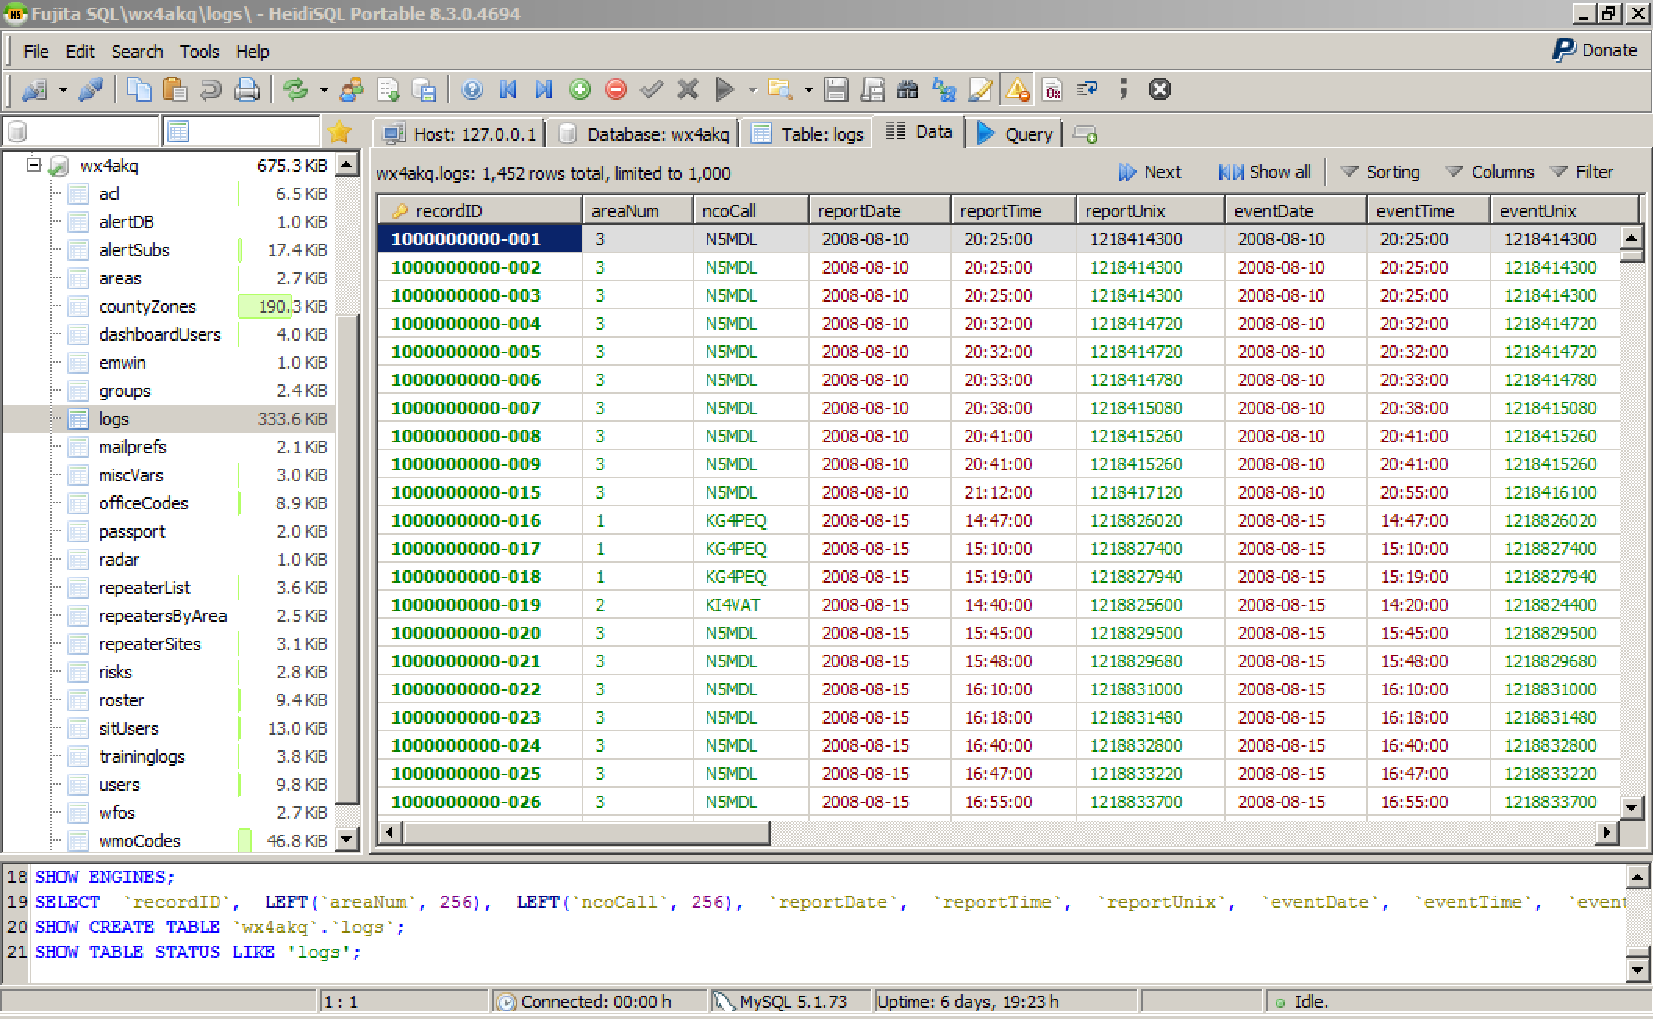
\includegraphics[width=\textwidth,keepaspectratio=true]{img/heidisql}
  \caption{HeidiSQL view of the \texttt{wx4akq/logs} table.\label{fig:heidisql}}
\end{figure}


To begin, download the \href{http://files.wx4akq.org/Software/MySQL\_Utilities/Portable\%20HeidiSQL.zip}{HeidiSQL Portable ZIP}\footnote{http://files.wx4akq.org/Software/MySQL\_Utilities/Portable\%20HeidiSQL.zip} file from our file library and decompress the file to a location on your computer.  This is a portable file so it will run directly from a USB drive if you prefer.

Double-click on the \texttt{Connect\_to\_Fujita.bat} file.  This file establishes a secure tunneled connection to our database server using Secure Shell (SSH), via the \href{http://www.chiark.greenend.org.uk/~sgtatham/putty/download.html}{Plink}\footnote{http://www.chiark.greenend.org.uk/~sgtatham/putty/download.html} application.

The first time you run this file on your computer you will be asked whether to add the remote key to your computer.  Doing so will enable you to more quickly connect in the future.

You will need the ``SSH Password'' for \texttt{wx4akq}.

\pagebreak
Once you have entered the proper credentials, you will see some gibberish followed by a command prompt from the server, like this:

\begin{verbatim}
Enter your server login credentials to establish the secure tunnel to Fujita.
Once you enter the password, you may then launch HeidiSQL.

To disconnect, simply close this window.

Using username "wx4akq".
wx4akq@fujita.wx4akq.org's password:
Last login: Fri May 30 21:12:17 2014 from 73.177.197.116
←]0;wx4akq@fujita:~←[?1034h[wx4akq@fujita ~]$
```
\end{verbatim}

You may then launch HeidiSQL by double-clicking the \texttt{heidisql.exe} icon.

Select the \texttt{Fujita SQL} profile on the left and then click the \texttt{Open} button.

Enter the user name \texttt{wx4akq} and the MySQL password for \texttt{wx4akq}.

To manipulate data, select the desired database in the left column.  In almost all cases you want the \texttt{wx4akq} database.  Then, select the desired table.  Tables will appear under the database name in the left column.  Finally, click the \texttt{Data} tab at the top to view the data contained in the selected table.  Figure \ref{fig:heidisql} shows a view of the data in the \texttt{wx4akq/logs} table as seen in HeidiSQL.

When you are finished, first exit HeidiSQL, then type \texttt{exit} into the remote session you established with the \texttt{Connect\_to\_Fujita.bat} file, or simply close the window.

\subsection{Mac OS X GUI Access with Sequel Pro}

One of several popular GUI's for MySQL access from Mac OS X is \href{http://www.sequelpro.com/}{Sequel Pro}\footnote{http://www.sequelpro.com/}.  To get started with Sequel Pro, download the \texttt{.dmg} file from the Sequel Pro web site, mount the disk image, and drag the application into your \texttt{Applications} folder.  Then double-click it to launch.

Figure \ref{fig:sequel-pro} shows a screen shot of Sequel Pro accessing our database on page \pageref{fig:sequel-pro}.

Download our \href{http://files.wx4akq.org/Software/MySQL\_Utilities/Sequel\_Pro\_Favorite\_Connection.plist}{Favorite Connection}\footnote{http://files.wx4akq.org/Software/MySQL\_Utilities/Sequel\_Pro\_Favorite\_Connection.plist} file from our file library and save it someplace convenient.  Then click the small gear icon in the lower left corner of the Sequel Pro window and select \texttt{Import}, then choose the file you just downloaded.

You will need the ``SSH password'' and ``MySQL password'' for \texttt{wx4akq}.  Enter those, and then click \texttt{Test Connection}.  If the tests succeed, click \texttt{Save Changes} and then click \texttt{Connect}.  For future connections, you can simply launch Sequel Pro, choose the favorite, and click \texttt{Connect}.

If the database you want is not automatically selected, you can choose it in the upper left corner.  In most cases, you want the \texttt{wx4akq} databsae.  Then select the desired table from the left column.

To manipulate the data in the table, select the table, then click the \texttt{Content} button at the top.

When you are done, simply close Sequel Pro to disconnect.

\subsection{iOS GUI Access with impathic MySQL Client}

MySQL access from iOS is possible with several different client applications, but here we will use the \href{https://itunes.apple.com/us/app/mysql-mobile-database-client/id397060484?mt=8}{impathic MySQL Client}\footnote{https://itunes.apple.com/us/app/mysql-mobile-database-client/id397060484?mt=8} (\$4.99) for access.

Launch the application and create a new connection.  Populate the following fields:

\begin{itemize}
\item \texttt{Database Host}: fujita.wx4akq.org
\item \texttt{User Name}: wx4akq
\item \texttt{Password}: (use the current ``MySQL password'')
\item \texttt{Database Name}: wx4akq
\item \texttt{Database Port}: 3306
\end{itemize}

Then tap on \texttt{Advanced}, toggle \texttt{Enable Compression} on, then tap \texttt{SSH Tunnel}.  Populate the following fields:

\begin{itemize}
\item \texttt{SSH Host}: fujita.wx4akq.org
\item \texttt{SSH Port}: 22
\item \texttt{SSH Username}: wx4akq
\item \texttt{SSH Password}: (use the current ``SSH password'')
\end{itemize}

Go back to the \texttt{Settings} screen, back to the \texttt{Create New Connection} screen, and then tap \texttt{Save} to store the settings.

You will be prompted to select a table, and can then view and edit the data within each table.

%%%%%%%%%%%%%%%%%%%%%%%%%%%%%%%%%%%%%%%%%%%%%%%%%%%%%%%%%%%%%%%%%%%%%%%%

\section{Repeater Database and Area Maps}

Our repeater database provides the data used to generate frequency listings on the SKYWARN web site as well as our map features, including embedded maps on the SKYWARN web site and the downloadable Keyhole Markup Language (KML) files.

The database is comprised of three MySQL tables stored within the \texttt{wx4akq} database on our server: \texttt{repeaterList}, \texttt{repeatersByArea}, and \texttt{repeaterSites}.  These databases are described in this document.

\subsection{repeaterSites table}

The \texttt{repeaterSites} table maintains information on the physical locations of the repeater sites, and this is the starting point for creation of any new repeater in our system.

There are four fields in the table:

\begin{itemize}
\item \texttt{comments}: This is a plain-language description of the repeater site for ease of identification.  This information is not embedded in any of our maps or displayed anywhere on our web sites.  It is for your reference only.

\item \texttt{coordType}:  Describes the mechanism by which the site coordinates have been determined.  This can be any of these values:
	\begin{enumerate}
	\item \texttt{exact}: Coordinates are representative of the exact location of the repeater site.
	\item \texttt{approx}: Coordinates are close to the repeater site but aren't exact. This coordinate type is usually utilized when a repeater owner does not want the exact location of the repeater to be known to the general public.
	\item \texttt{city}: Coordinates represent the approximate geographic center of the town/city in which the repeater is located.  This coordinate type is typically used if a repeater's location cannot be determined.
	\end{enumerate}
\item \texttt{lat} and \texttt{lon}: Decimal coordinates representing the repeater's location.
\end{itemize}

Each row in the \texttt{repeaterSites} table is assigned an auto-increment \texttt{id} field which is referenced by the other tables in the database.

\subsection{repeaterList table}

The \texttt{repeaterList} table contains the functional data about each repeater in the SKYWARN system, as well as any comments to be displayed on the web site and on our maps.  A plain-language \texttt{location} field is included but the maps are generated based on the coordinates of the machine as specified in the \texttt{repeaterSites} table and referenced by the \texttt{siteId} field in the \texttt{repeaterList} table.

The fields in \texttt{repeaterList} are:

\begin{itemize}
\item \texttt{callSign}:  The repeater's call sign.
\item \texttt{frequency}:  The frequency in MHz.
\item \texttt{location}:  Plain-language description of the location of the repeater in print-ready format, generally just the town/city and state, ie., ``Richmond, VA''
\item \texttt{pl}:  The PL tone in Hz.  \texttt{null} if none.
\item \texttt{echolink}:  The numeric Echolink node assigned to the repeater.  \texttt{null} if none.
\item \texttt{irlp}:  The IRLP node assigned to the repeater.  \texttt{null} if none.
\item \texttt{comments}:  Brief comments about the repeater, if any, which will be displayed on the web site and in our maps.
\item \texttt{siteId}:  The number of the corresponding \texttt{id} value from the \texttt{repeaterSites} table.
\end{itemize}

\subsection{repeatersByArea table}

The \texttt{repeatersByArea} table handles the assignment of each repeater to one or more SKYWARN areas and also specifies the role of the repeater.  The three fields in the \texttt{repeatersByArea} table are:

\begin{itemize}
\item \texttt{areaNum}:  The numeric SKYWARN area number for the repeater assignment.
\item \texttt{repeaterId}:  The numeric identifier of the repeater, based on the \texttt{id} field in the \texttt{repeaterList} table.
\item \texttt{repeaterType}: Numeric role code indicating the repeater's role in that area. May be one of the following:
	\begin{enumerate}
	\item \texttt{1}: Primary Repeater
	\item \texttt{2}: Linked Repeater (linked to primary)
	\item \texttt{3}: Subnet Repeater
	\item \texttt{4}: Backup Repeater
	\item \texttt{5}: Auxiliary Repeater
	\item \texttt{6}: VoIP-Only Repeater (routes in to our Echolink/IRLP nets)
	\end{enumerate}
\end{itemize}

One repeater may be assigned to more than one area.  For example, repeater \#6 may be a primary for Area 1 and a backup for Area 2.  In that case, the following MySQL queries would be used:

\begin{minted}[linenos=true]{mysql}
INSERT INTO repeatersByArea
	(areaNum, repeaterId, repeaterType)
	VALUES
	(1, 6, 1);
INSERT INTO repeatersByArea
	(areaNum, repeaterId, repeaterType)
	VALUES
	(2, 6, 2);
\end{minted}

...which assigns \texttt{repeaterType} 2 (Backup Repeater) to Area 2 and \texttt{repeaterType} 1 (Primary Repeater) to Area 1.

\orangebox{Shortcut!}{Rather than manipulate the databases directly with raw MySQL queries as shown here, there are number of graphical user interfaces (GUI's) to make MySQL modifications much easier.  See our section called \nameref{database-server} starting on page \pageref{database-server} for information about accessing the MySQL server via both console and graphical interfaces.}

\subsection{Adding New Repeaters}

The process of adding a new repeater involves three steps:

\begin{enumerate}
\item Create a new repeater site in \texttt{repeaterSites} \emph{or} obtain the \texttt{id} of an existing site at the same location by querying \texttt{repeaterSites}.
\item Create a new row in \texttt{repeaterList} with the details of the repeater.
\item Create a new row in \texttt{repeatersByArea} assigning the repeater to an area and establishing its role.
\end{enumerate}

This is extremely easy to accomplish using a MySQL GUI.

Here is a sample query sequence for making the changes by hand:

\begin{minted}[linenos=true]{mysql}
# Create the entry in repeaterSites
INSERT INTO repeaterSites
	(comments,coordType,lat,lon)
	VALUES
	("AB1CDE Repeater","exact",36.43567,-76.6789);

# Get the `id` value to use as `siteId` in repeaterList.
# We will assume this returns `22` in this example.
SELECT LAST_INSERT_ID();

# Create the entry in repeaterList
INSERT INTO repeaterList
	(callSign, frequency, location, pl, irlp, siteId)
	VALUES
	("AB1CDE", 146.73, "MyTown, VA", 100, 4567, 22);

# Get the `id` to use as `repeaterId` in repeatersByArea.
# We will assume this returns `31` in this example.
SELECT LAST_INSERT_ID();

# Create the entries in repeatersByArea
INSERT INTO repeatersByArea
	(areaNum, repeaterId, repeaterType)
	VALUES
	(2, 31, 1);
INSERT INTO repeatersByArea
	(areaNum, repeaterId, repeaterType)
	VALUES
	(6, 31, 2);
\end{minted}

\subsection{Updating the Web Site}

Once all three databases are populated with the repeater data, all internal and external SKYWARN web sites will immediately display the repeater data.

There is no delay in updating the information on the sites.

\subsection{Updating the Maps}

Maps are generated from KML files produced from the information in our databases.  A server-side script automatically regenerates these maps once every 2 hours.

To expedite map updates, manually start KML generation by running the \texttt{mkkml.sh} script in the public web folder:

\begin{minted}[linenos=true]{text}
/var/www/sites/pub/mkkml.sh
\end{minted}

Once the script completes, KML files for all areas will be updated.  Online map displays will now reflect the new information.


\end{document}